% Options for packages loaded elsewhere
\PassOptionsToPackage{unicode}{hyperref}
\PassOptionsToPackage{hyphens}{url}
%
\documentclass[
]{article}
\usepackage{lmodern}
\usepackage{amssymb,amsmath}
\usepackage{ifxetex,ifluatex}
\ifnum 0\ifxetex 1\fi\ifluatex 1\fi=0 % if pdftex
  \usepackage[T1]{fontenc}
  \usepackage[utf8]{inputenc}
  \usepackage{textcomp} % provide euro and other symbols
\else % if luatex or xetex
  \usepackage{unicode-math}
  \defaultfontfeatures{Scale=MatchLowercase}
  \defaultfontfeatures[\rmfamily]{Ligatures=TeX,Scale=1}
\fi
% Use upquote if available, for straight quotes in verbatim environments
\IfFileExists{upquote.sty}{\usepackage{upquote}}{}
\IfFileExists{microtype.sty}{% use microtype if available
  \usepackage[]{microtype}
  \UseMicrotypeSet[protrusion]{basicmath} % disable protrusion for tt fonts
}{}
\makeatletter
\@ifundefined{KOMAClassName}{% if non-KOMA class
  \IfFileExists{parskip.sty}{%
    \usepackage{parskip}
  }{% else
    \setlength{\parindent}{0pt}
    \setlength{\parskip}{6pt plus 2pt minus 1pt}}
}{% if KOMA class
  \KOMAoptions{parskip=half}}
\makeatother
\usepackage{xcolor}
\IfFileExists{xurl.sty}{\usepackage{xurl}}{} % add URL line breaks if available
\IfFileExists{bookmark.sty}{\usepackage{bookmark}}{\usepackage{hyperref}}
\hypersetup{
  hidelinks,
  pdfcreator={LaTeX via pandoc}}
\urlstyle{same} % disable monospaced font for URLs
\usepackage[margin=1in]{geometry}
\usepackage{longtable,booktabs}
% Correct order of tables after \paragraph or \subparagraph
\usepackage{etoolbox}
\makeatletter
\patchcmd\longtable{\par}{\if@noskipsec\mbox{}\fi\par}{}{}
\makeatother
% Allow footnotes in longtable head/foot
\IfFileExists{footnotehyper.sty}{\usepackage{footnotehyper}}{\usepackage{footnote}}
\makesavenoteenv{longtable}
\usepackage{graphicx,grffile}
\makeatletter
\def\maxwidth{\ifdim\Gin@nat@width>\linewidth\linewidth\else\Gin@nat@width\fi}
\def\maxheight{\ifdim\Gin@nat@height>\textheight\textheight\else\Gin@nat@height\fi}
\makeatother
% Scale images if necessary, so that they will not overflow the page
% margins by default, and it is still possible to overwrite the defaults
% using explicit options in \includegraphics[width, height, ...]{}
\setkeys{Gin}{width=\maxwidth,height=\maxheight,keepaspectratio}
% Set default figure placement to htbp
\makeatletter
\def\fps@figure{htbp}
\makeatother
\setlength{\emergencystretch}{3em} % prevent overfull lines
\providecommand{\tightlist}{%
  \setlength{\itemsep}{0pt}\setlength{\parskip}{0pt}}
\setcounter{secnumdepth}{-\maxdimen} % remove section numbering
\usepackage[USenglish]{babel}
\usepackage{fancyhdr}
\pagestyle{fancy}
\renewcommand{\sectionmark}[1]{\markright{#1}}
\fancyhf{}
\lhead{\textcolor{red}{PRE-PRINT: NOT PEER-REVIEWED}}
\rhead{{\today}}
\cfoot{{\thepage}}
\usepackage[T1]{fontenc}
\usepackage{bm}
\usepackage{mathpazo}
\usepackage{lscape}
\usepackage{pdfpages}
\newcommand{\blandscape}{\begin{landscape}}
\newcommand{\elandscape}{\end{landscape}}
\usepackage{tabularx}
\usepackage{titlesec}
\usepackage{graphicx,xcolor}
\usepackage{wrapfig}
\usepackage{amssymb}
\usepackage{amsmath}
\usepackage{hyperref}
\hypersetup{ colorlinks=true, citecolor = blue, linkcolor=blue, urlcolor=blue}
\usepackage{esint}
\usepackage{paralist}
\usepackage{outlines}
\newcommand{\I}{\textrm{I}}
\newcommand{\N}{\mathcal{N}}
\newcommand{\D}{\textrm{D}}
\newcommand{\E}{\mathbb{E}}
\setlength{\parskip}{1em}%0.5\baselineskip
\setlength{\parindent}{0pt}
\linespread{1.15}
\titleformat*{\section}{\Large\scshape\bfseries}
\titleformat*{\subsection}{\large\scshape\bfseries}
\titleformat*{\subsubsection}{\bfseries}
\titleformat*{\paragraph}{\bfseries}
\titleformat*{\subparagraph}{\bfseries}
\renewcommand{\thesection}{\Roman{section}.}%1.A.assubsections
\renewcommand{\thesubsection}{\Alph{subsection}.}%1.A.assubsections
\titlespacing{\section}{0pt}{2pt}{3pt}
\titlespacing{\subsection}{0pt}{2pt}{2pt}
\titlespacing{\subsubsection}{0pt}{0pt}{0pt}
\titlespacing{\paragraph}{0pt}{1pt}{5pt}
\titlespacing{\subparagraph}{10pt}{1pt}{5pt}
\usepackage{hyperref}
\usepackage[font={footnotesize}]{subcaption}
\usepackage[font={footnotesize}]{caption}
\usepackage{caption,setspace}
\captionsetup{font={stretch=1}}
\captionsetup[figure]{font=footnotesize,labelfont=footnotesize}
\usepackage{tabto}
\def\quoteattr#1#2{\setbox0=\hbox{#2}#1\tabto{\dimexpr\linewidth-\wd0}\box0}
\makeatletter
\newcommand{\pushright}[1]{\ifmeasuring@#1\hfill$\displaystyle#1$\fi\ignorespaces}
\makeatother
\newcommand{\FixMe}[1]{\textcolor{orange}{[#1]}}
\newcommand{\Comment}[1]{\textcolor{purple}{\textit{[#1]}}}
\newcommand{\Quickwin}{{\color{blue}{$\bigstar$}}}
\usepackage{letltxmacro}
\LetLtxMacro\Oldfootnote\footnote
\newcommand{\EnableFootNotes}{\LetLtxMacro\footnote\Oldfootnote}
\newcommand{\DisableFootNotes}{\renewcommand{\footnote}[2][]{\relax}}
\makeatother
\graphicspath{{../Output/"}}

\author{}
\date{\vspace{-2.5em}}

\begin{document}

\begin{center} 
\textbf{\scshape \LARGE Passing the Test: A model-based analysis of safe school-reopening strategies}\\  \vspace{2mm}
{\large Alyssa Bilinski MS\footnote{Interfaculty Initiative in Health Policy, Harvard Graduate School of Arts and Sciences (abilinski@g.harvard.edu)} $\cdot$ Joshua A. Salomon, PhD\footnote{Center for Health Policy \& Center for Primary Care and Outcomes Research, Stanford University School of Medicine} $\cdot$ John Giardina$^1$ }\\
{\large Andrea Ciaranello MD, MPH\footnote{Medical Practice Evaluation Center and Division of Infectious Disease, Massachusetts General Hospital, Harvard Medical School} $\cdot$ Meagan C. Fitzpatrick, PhD\footnote{Center for Vaccine Development and Global Health, University of Maryland School of Medicine (meagan.fitzpatrick@som.umaryland.edu)}} \\
\end{center}

\vspace{-0.50em}
\bigskip

\begin{abstract}

\noindent \textbf{Background.} The COVID-19 pandemic has induced historic educational disruptions.  In December 2020, at least two-thirds of US public school students were not attending full-time in-person education.  The Biden Administration has expressed that reopening schools is a priority. \\

\noindent \textbf{Objective.} To compare risks of SARS-COV-2 transmission in schools across different school-based prevention strategies and levels of community transmission. \\

\noindent \textbf{Design.} We developed an agent-based network model to simulate transmission in elementary and high school communities, including home, school, and inter-household interactions. \\

\noindent \textbf{Setting.} We parameterized school structure based on average US classrooms, with elementary schools of 638 students and high schools of 1,451 students.  We varied daily community incidence from 1 to 100 cases per 100,000 population. \\

\noindent \textbf{Patients (or Participants).} We simulated students, faculty/staff, and adult household members. \\

\noindent \textbf{Interventions.} We evaluated isolation of symptomatic individuals, quarantine of an infected individual’s contacts, reduced class sizes, alternative schedules, staff vaccination, and weekly asymptomatic screening. \\

\noindent \textbf{Measurements.} We projected transmission among students, staff and families during one month following introduction of a single infection into a school. We also calculated the number of infections expected for a typical 8-week quarter, contingent on community incidence rate. \\

\noindent \textbf{Results.} School transmission risk varies according to student age and community incidence and is substantially reduced with effective, consistent mitigation measures.  Nevertheless, when transmission occurs, it may be difficult to detect without regular, frequent testing due to the subclinical nature of most infections in children.  Teacher vaccination can reduce transmission to staff, while asymptomatic screening both improves understanding of local circumstances and reduces transmission, facilitating five-day schedules at full classroom capacity. \\

\noindent \textbf{Limitations.} There is uncertainty about susceptibility and infectiousness of children and low precision regarding the effectiveness of specific prevention measures, particularly with emergence of new variants. \\

\noindent \textbf{Conclusion.} With controlled community transmission and moderate school-based prevention measures, elementary schools can open with few in-school transmissions, while high schools require more intensive mitigation.  Asymptomatic screening can both reduce transmission and provide useful information for decision-makers. \\

\noindent \textbf{Acknowledgements.} The authors were supported by the Centers for Disease Control and Prevention though the Council of State and Territorial Epidemiologists (NU38OT000297-02; AB, JAS), the National Institute of Allergy and Infectious Diseases (R37AI058736-16S1; ALC and K01AI141576; MCF), the National Institute on Drug Abuse (3R37DA01561217S1; JAS).  The papers' contents are solely the responsibility of the authors and do not necessarily represent the official views of the funders.  Model code is available at \url{https://github.com/abilinski/BackToSchool2}{https://github.com/abilinski/BackToSchool2}.

\end{abstract}

\doublespacing

\hypertarget{introduction}{%
\section{Introduction}\label{introduction}}

COVID-19 prompted an unprecedented number of school closures during the
spring of 2020. All 50 states recommended or mandated public school
closures, impacting at least 124,000 US schools and over 55.1 million
students (\protect\hyperlink{ref-noauthor_map_2020}{1}). Reopenings have
proven challenging, and as of December 9, 2020, only 33\% of K-12
students were offered full-time in-person learning, a figure that has
since the fall (\protect\hyperlink{ref-noauthor_k-12_nodate}{2}). Where
in-person schooling has been offered, a substantial percentage of
families have opted out, including more than half in parts of Orange
County, Florida and 70\% in New York City
(\protect\hyperlink{ref-noauthor_more_nodate}{3},\protect\hyperlink{ref-shapiro_when_2020}{4}).
Many parents and advocates have objected strongly to school closures
(\protect\hyperlink{ref-shapiro_how_2020}{5}), and the Biden
administration has stated a priority to rapidly facilitate safe,
in-person school reopening in a manner that gains the trust of students,
parents, and teachers
(\protect\hyperlink{ref-noauthor_combating_nodate}{6}).

Debates around school reopening have been heated and often invoked
seemingly contradictory evidence about its safety. For example, a number
of well-studied cases in school settings have found minimal secondary
transmission
(\protect\hyperlink{ref-macartney_transmission_2020}{7}--\protect\hyperlink{ref-yung_novel_nodate}{9}).
Nevertheless, significant school clusters have also been documented,
particularly in Israel and in parts of the United States
(\protect\hyperlink{ref-stein-zamir_large_2020}{10}--\protect\hyperlink{ref-torres_sars-cov-2_nodate}{12}),
and some observational studies have suggested that school closures may
have substantially reduced transmission
(\protect\hyperlink{ref-auger_association_2020}{13}). Proponents of
reopening schools point to evidence that COVID-19 is most often mild in
children (\protect\hyperlink{ref-dong_epidemiology_2020}{15}), while
others have expressed concern that infection may lead to severe outcomes
in some children, as well as among staff, families, and the community.
The discord plays out similarly on a macro scale: a number of Asian and
European countries reopened schools with physical distancing when
community transmission was low and reported negligible increases in
transmission
(\protect\hyperlink{ref-noauthor_reopening_2020}{16},\protect\hyperlink{ref-pancevski_is_2020}{17}).
Some, including France, the United Kingdom, and Ireland, kept schools
open during the fall wave and have reversed surging transmission by
closing other sectors, although the latter two closed schools following
the emergence of variant B.1.1.7.
(\protect\hyperlink{ref-vogel_as_2020}{18},\protect\hyperlink{ref-staton_european_2021}{19}).
Others, such as Austria, the Czech Republic, and South Korea, have
closed schools to address rising case burdens
(\protect\hyperlink{ref-vogel_as_2020}{18}).

Nevertheless, there is little debate that the benefits of in-person
education are substantial, particularly amidst reports of high levels of
remote absenteeism, increased depression, anxiety, and suicidality, and
parent concerns around educational quality
(\protect\hyperlink{ref-polikoff_surveys_2020}{20}--\protect\hyperlink{ref-leeb_mental_2020}{22}).
Beyond educational and mental health outcomes, opening schools can also
improve access to social services for children and labor market outcomes
for working parents, especially women
(\protect\hyperlink{ref-hess_widespread_2020}{23}--\protect\hyperlink{ref-soland_impact_2020}{27}).
In order to do so safely, it is critical to take a comprehensive account
of the full array of sometimes contradictory evidence and identify a
robust set of policies to mitigate risks.

We simulated SARS-CoV-2 transmission dynamics in elementary and high
schools, to characterize how school transmission may occur either as
isolated or sustained outbreaks. While several recent papers have
discussed the impact of school reopening on the broader epidemic under
different mitigation strategies
(\protect\hyperlink{ref-cohen_schools_2020}{28}--\protect\hyperlink{ref-head_effect_2020}{30}),
our work focused on the risk that transmission will occur on a school
campus and spread to households of students and educators/staff. We
emphasize uncertainty in transmission risk (rather than focusing on the
average) as well as the observability of infections to school and public
health staff, allowing us to reconcile apparent contradictions in the
evidence. We evaluated outcomes under varying combinations of community
incidence, in-classroom mitigation efforts, testing practices, and staff
vaccination. We project that consistently implemented mitigation,
including masking and distancing, can drastically reduce the risk of
school-based transmission, particularly in elementary schools.
Nevertheless, high rates of subclinical disease, especially in children
and adolescents, may render transmission difficult to connect to schools
via contact tracing, and imperfect implementation of mitigation
strategies or stochastic error (``bad luck'') can produce outbreaks even
in well-managed systems. We find that teacher vaccination and
asymptomatic screening can help support safe return to 5-day schooling
for all children with only targeted closures, even amidst moderate
ongoing community transmission.

\hypertarget{methods}{%
\section{Methods}\label{methods}}

We developed an age-specific, agent-based network model of COVID-19
transmission in elementary and high school communities (Figure
\ref{fig1}). We incorporated interactions within schools and homes, as
well as those between households in childcare or social interactions
outside of the school setting. Because data are particularly
inconclusive on transmission among middle school-aged children, we did
not model middle schools explicitly; accumulating evidence suggests that
they may be more similar to high schools than elementary schools with
respect to susceptibility and infectiousness
(\protect\hyperlink{ref-park_early_nodate}{31},\protect\hyperlink{ref-cdc_covid-19_2020}{32}).

\hypertarget{scenarios}{%
\subsection{Scenarios}\label{scenarios}}

We simulated different combinations of interventions, incorporating
strategies that target the three axes of general infection control in
schools; COVID-19-specific countermeasures; and scheduling/cohorting
with parameters detailed in Table \ref{tab:tbl1}.

\medskip

\hypertarget{general-infection-control-in-schools}{%
\subsubsection{General infection control in
schools:}\label{general-infection-control-in-schools}}

\begin{enumerate}
\def\labelenumi{\arabic{enumi}.}
\tightlist
\item
  \textbf{Low uptake:} Schools implemented no or minimal general
  infection control measures, such as masking and distancing.
\item
  \textbf{Medium uptake:} Schools implemented masking and distancing,
  and adherence was moderate such that the risk transmission given
  infectious contact was \(\frac{2}{3}\) that experienced in a school
  with low uptake.
\item
  \textbf{High uptake:} Schools implemented masking and distancing and
  adherence was high, such that the risk of transmission given
  infectious contact was \(\frac{1}{3}\) that experienced in a school
  with low uptake.
\end{enumerate}

\medskip

\hypertarget{covid-19-specific-countermeasures}{%
\subsubsection{COVID-19-specific
countermeasures:}\label{covid-19-specific-countermeasures}}

\begin{enumerate}
\def\labelenumi{\arabic{enumi}.}
\tightlist
\item
  \textbf{Symptom-based self-isolation (“Symptomatic isolation”):}
  Individuals in the school were screened for symptoms daily, and those
  who developed clinically-recognizable symptoms did not attend school.
\item
  \textbf{Diagnostic testing plus classroom notification (“Classroom quarantine”):}
  Individuals who developed symptoms were isolated and immediately
  tested. The school received results within a day, and all classroom(s)
  associated with an individual who tested positive were notified and
  closed for 10 days, per updated/recent CDC guidelines (32).
\item
  \textbf{Teacher vaccination with an infection-blocking vaccine (“Staff vaccination”):}
  In addition to classroom quarantine, teacher susceptibility was
  reduced to 33\% of baseline, roughly assuming that 75\% of teachers
  receive an infection-blocking vaccine with 90\% effectiveness
  (\protect\hyperlink{ref-gallup_inc_willingness_2020}{33}--\protect\hyperlink{ref-polack_safety_2020}{35}).
\item
  \textbf{Weekly asymptomatic screening (“Weekly screening”):} In
  addition to classroom quarantine, asymptomatic students and/or staff
  at each school were tested weekly. We assumed test acceptance was
  90\%, sensitivity was 90\% during the infectious period, and results
  were available within 24 hours. Upon receipt of a positive result,
  infected individuals isolated outside of school for 10 days based on
  CDC guidelines, and siblings and classroom members of an individual
  who tests positive were notified and quarantined for 10 days.
\end{enumerate}

\medskip

\hypertarget{schedulingcohorting}{%
\subsubsection{Scheduling/Cohorting:}\label{schedulingcohorting}}

\begin{enumerate}
\def\labelenumi{\arabic{enumi}.}
\tightlist
\item
  \textbf{5-day schedule:} This scenario simulated a traditional 5-day,
  in-person learning schedule, allowing for classroom contacts,
  staff-staff interactions (10 per day), and random contacts between
  school members (20 per day). Related arts and special education
  teachers had revolving contact with 5 classrooms per day.
\item
  \textbf{Cohorting:} This scenario again assumed 5 days of in-person
  learning for all students, but with restricted out-of-classroom
  contacts, including separation of classes for lunch and recess.
  Students and primary teachers continued to have sustained classroom
  contacts. We assumed a 50\% decrease in the number out-of-classroom
  contacts during the school day and that related arts were taught
  remotely.
\item
  \textbf{Half class sizes:} All students attended school five days per
  week, but in classes of half their typical size. To accommodate this,
  the number of teachers was doubled. Limited contacts as in (2) were
  also maintained.
\item
  \textbf{Hybrid scheduling (A/B):} Classes were subdivided into 2
  cohorts, and students attended school for 2 days per week, either
  Monday/Tuesday or Thursday/Friday. Elementary school children in the
  same household attending the same school were sorted into the same
  cohort. All staff were physically present each instructional day. In
  sensitivity analysis, we considered alternative hybrid schedules.
  Limited contacts as in (2) were also maintained.
\end{enumerate}

\hypertarget{model-structure}{%
\subsection{Model structure}\label{model-structure}}

\hypertarget{households}{%
\subsubsection{Households}\label{households}}

We generated a set of synthetic households from US population data
(\protect\hyperlink{ref-wheaton_us_2014}{36}) (Supplement). For
elementary schools, we sampled from households containing at least one
child aged 5 to 10 to identify siblings attending the same school. For
high schools, we sampled from households with students aged 14 to 17.
For each student, we included two adults in the household, based on the
average number of household members over 25. For each staff member, we
also included a household adult contact, representing a partner or
roommate with whom they had close contact.

\medskip

\hypertarget{elementary-schools}{%
\subsubsection{Elementary schools}\label{elementary-schools}}

To simulate a representative school, we identified the average school
size weighted by student population
(\protect\hyperlink{ref-noauthor_digest_nodate}{37}). We simulated an
average-sized elementary school of 638 pupils from 500 households, of
which 114 households had more than one child in the school. We set five
classes per grade level, an average class size of 21 children, and one
primary teacher per class. We also incorporated 30 additional staff, to
reflect roles such as administrators, counselors, cafeteria staff,
custodians, special education teachers, and teachers of related arts (or
`specials', e.g.~music and art). These adults were assigned either
in-classroom roles (n = 15, including special education and related arts
teachers who are in rotating contact with entire classes of students) or
out-of-classroom roles (n = 15, interacting with fewer individuals
outside the classroom setting).

\medskip

\hypertarget{high-schools}{%
\subsubsection{High schools}\label{high-schools}}

We simulated an average-sized high school of 1451 students in 1225
households, with 142 households having more than one student in the
school (\protect\hyperlink{ref-noauthor_digest_nodate}{37}). Students
rotated among 8 class periods per day (23 students and 1 teacher), with
the distribution of students to class periods chosen randomly within
grade levels but repeated daily for the full simulation. The high school
had 45 additional staff with out-of-classroom roles and 15 with
in-classroom roles. In both elementary and high schools, teachers were
modeled to have additional staff contacts per day (e.g., contacts in
break rooms or offices).

\medskip

\hypertarget{out-of-school-interactions}{%
\subsubsection{Out-of-school
interactions}\label{out-of-school-interactions}}

Reflecting social interactions and out-of-school childcare, our base
case analysis assumed that each family interacted with 1 additional
family on each day they did not attend school, randomly reassorted each
day. We varied this number in sensitivity analysis from 0 to 9 families
per day out of school. We assume that when families mix, no more than 2
adults attend at a given time, who are randomly selected.

\hypertarget{transmission-and-epidemiological-parameters}{%
\subsection{Transmission and epidemiological
parameters}\label{transmission-and-epidemiological-parameters}}

At each daily time-step, we modeled dyadic interactions between
individuals according to household, classroom, school, and childcare
relationships, drawing parameter values from the distributions specified
in Table \ref{tab:tbl1}. A SARS-CoV-2-infected individual i transmitted
to susceptible individual j at time t with Bernoulli probability equal
to: \begin{align*}
p_{ijt}= c_{ijkt} q_k s_j r_i a_i d_i 
\end{align*} where \(c_{ijk}\) was an indicator variable equal to 1 if
individuals \(i\) and \(j\) had contact type \(k\) at time \(t\),
\(q_k\) was the probability of transmission given one day of contact
type \(k\), \(r_i\) was the relative infectiousness of individual \(i\)
(compared to full adult infectiousness), \(s_j\) was the relative
susceptibility of individual \(j\) (compared to full adult
infectiousness), and \(a_i\) indicated whether individual \(i\) had
asymptomatic disease and \(d_i\) was a dispersion factor representing
individual-level heterogeneity in transmissibility.

\medskip

\hypertarget{secondary-attack-rate-sar-q_k}{%
\subsubsection{\texorpdfstring{Secondary attack rate (SAR)
(\(q_k\))}{Secondary attack rate (SAR) (q\_k)}}\label{secondary-attack-rate-sar-q_k}}

Secondary attack rates (SARs) for SARS-CoV-2, the probability that a
person with SARS-CoV-2 transmitted it to an individual they contacted,
vary by contact type: household, classroom, random school, and
out-of-school social/childcare contacts. Household SARs have been most
frequently estimated in a number of contact tracing studies. While there
is substantial variation across geographic locations, likely
corresponding to cultural norms and precautions adopted, we assumed a
20\% household adult-adult secondary attack rate over the full duration
of an infection, translating to approximately 4\% per day
(\protect\hyperlink{ref-madewell_household_2020}{38},\protect\hyperlink{ref-fung_household_2020}{39}).
This assumed minimal in-home quarantine measures but less household
mixing than during full shelter-in-place orders.

We used the SAR from household contact tracing studies as a rough proxy
for the per-day adult-adult attack rate in non-household settings,
following close sustained contact in the absence of interventions such
as masks and distancing. For school based transmission, we allowed
adult-adult attack rates to reach up to 3\% per day for scenarios with
low uptake of masks and distancing, a downward adjustment from the
household attack rate to account for less close contact in professional
settings. We developed the scale of reductions in transmission from
mitigation measures in line with observations from in household settings
with high prevention measures
(\protect\hyperlink{ref-park_early_nodate}{31},\protect\hyperlink{ref-cheng_contact_2020}{40})
and based on effectiveness analyses for measures like masks
(\protect\hyperlink{ref-clapp_evaluation_2020}{41},\protect\hyperlink{ref-chu_physical_2020}{42}).

\medskip

\hypertarget{relative-susceptibility-s_i-and-infectiousness-in-children-r_i}{%
\subsubsection{\texorpdfstring{Relative susceptibility (\(s_i\)) and
infectiousness in children
(\(r_i\))}{Relative susceptibility (s\_i) and infectiousness in children (r\_i)}}\label{relative-susceptibility-s_i-and-infectiousness-in-children-r_i}}

Household contact tracing studies suggest that adults are likely more
susceptible to COVID-19 and more apt to transmit it when infected than
children, although data, particularly for the latter, are equivocal and
limited by availability and timing of testing
(\protect\hyperlink{ref-viner_susceptibility_2020}{43}). Several sources
indicate that any differences wane by the teenage years, possibly as
early as age 10
(\protect\hyperlink{ref-fontanet_sars-cov-2_2020}{8},\protect\hyperlink{ref-stein-zamir_large_2020}{10},\protect\hyperlink{ref-park_early_nodate}{31},\protect\hyperlink{ref-dattner_role_2020}{44},\protect\hyperlink{ref-fontanet_cluster_2020}{45}).
We assumed that elementary school children were half as susceptible as
adults while high school children were equally susceptible. Data are
similarly limited to inform transmission from children with COVID-19. We
further specified that elementary school children are half as infectious
as adults and high school students were equally as infectious as adults
(\protect\hyperlink{ref-park_early_nodate}{31},\protect\hyperlink{ref-dattner_role_2020}{44}).
We varied these assumptions in sensitivity analyses. We discuss the data
underlying this assumptions as well as comparisons to other modeling
work and documented in-school transmissions in the Supplement.

\medskip

\hypertarget{asymptomatic-transmission-a_i-and-overdispersion-d_i}{%
\subsubsection{\texorpdfstring{Asymptomatic transmission (\(a_i\)) and
overdispersion
(\(d_i\))}{Asymptomatic transmission (a\_i) and overdispersion (d\_i)}}\label{asymptomatic-transmission-a_i-and-overdispersion-d_i}}

We assumed that individuals with fully asymptomatic disease transmit
COVID-19 at half the rate of those with any symptoms
(\protect\hyperlink{ref-byambasuren_estimating_2020}{46}). While
reported heterogeneity in transmission may be partially driven by
differences in contact rates, we sample individual transmissibility
according to a lognormal distribution to allow for some variation by
individual characteristics (e.g.~viral load) in adults who have been
more widely identified as potential superspreaders
(\protect\hyperlink{ref-kerr_covasim_2020}{47},\protect\hyperlink{ref-endo_estimating_2020}{48}).

\hypertarget{model-implementation}{%
\subsection{Model implementation}\label{model-implementation}}

We first evaluated the downstream impact of a single infectious
individual. We randomly designated one member of the school community as
infected, starting on a random day of the week. We assessed the spread
of the virus over 30 days, as in most cases either all infections were
resolved over that time horizon or the spread was sufficiently large
that additional public health measures (e.g.~school closures) would be
expected to be adopted during that time. For each scenario, we ran our
model 2000 times and summarized:

\begin{enumerate}
\def\labelenumi{\arabic{enumi}.}
\tightlist
\item
  Mean number of infections generated in the school over 30 days after
  index case
\item
  Percentage of scenarios without transmission from the index case
\item
  Percentage of scenarios with more than 5 in-school transmissions
\end{enumerate}

We also describe the composition of secondary cases (proportion
occurring in students, staff, and family members of students or staff).

Second, we quantified SARS-CoV-2 infections among our school population
across a typical school quarter, given a constant community incidence.
On each day over 8 weeks, every susceptible individual has a probability
of becoming spontaneously infected outside of school that is equivalent
to an age-adjusted community per capita daily incidence, distinct from
their contact-dependent risk within the school network. When schools are
remote, we assumed, similar to the analysis of hybrid schools, that each
family interacted with 1 additional family on each day they did not
attend school. For each scenario, we summarized:

\begin{enumerate}
\def\labelenumi{\arabic{enumi}.}
\tightlist
\item
  Cumulative incidence overall and by type
\item
  Incremental incidence compared to remote learning
\end{enumerate}

\textbf{Transmission control threshold:} We defined a reopening strategy
as controlling transmission in a group (students, educators/staff, or
families) if it resulted in less than a one point increase in the
percentage of the group which became infected, compared to remote
learning. This threshold is consistent with thresholds used by similar
papers and with the generally consensus objective of minimizing
in-school transmission
(\protect\hyperlink{ref-head_effect_2020}{30},\protect\hyperlink{ref-noauthor_schools_nodate}{49}).

\hypertarget{results}{%
\section{Results}\label{results}}

\hypertarget{in-school-transmission-after-the-introduction-of-a-single-infection}{%
\subsection{In-school transmission after the introduction of a single
infection}\label{in-school-transmission-after-the-introduction-of-a-single-infection}}

\hypertarget{in-school-mitigation}{%
\subsubsection{In-school mitigation}\label{in-school-mitigation}}

In elementary schools with low mitigation and symptomatic isolation
under a 5-day schedule, we projected an average of 2 secondary cases
over 30 days following infection of a single index case (Figure
\ref{fig2}A, left panel). This fell to 1 case with medium mitigation,
and further to 0.4 cases with high mitigation. Under symptomatic
isolation, transmission was most reduced by replacing the 5-day schedule
with an A/B schedule (to 0.1-0.4 secondary cases depending on uptake of
in-school prevention). With high mitigation, there were on average
\textless0.5 secondary transmissions per case in all scenarios.

In high schools, where we specified that students acquired and
transmitted infection at the same rate as adults, we found the potential
for larger outbreaks after a single introduction into the school,
particularly when uptake of in-school prevention was low (Figure
\ref{fig2}B). For example, with low mitigation and classroom quarantine
under a 5-day schedule, we projected 22 secondary cases in the school
community over a 30-day period (in the absence of public health
responses that would likely ensue before 30 days, such as school
closure). High uptake of in-school mitigation reduced this markedly, to
1.8 cases.

\hypertarget{quarantine-teacher-vaccination-and-screening}{%
\subsection{Quarantine, teacher vaccination, and
screening}\label{quarantine-teacher-vaccination-and-screening}}

In elementary schools, where children were assumed to be less
susceptible and infectious, classroom quarantine had a modest impact on
transmission, although its impact was greater if the index case was a
teacher (Figure \ref{figs1}). In high schools, classroom quarantine
reduced projected average transmissions by a factor of 0.23 under low
mitigation, but had smaller impact with high mitigation. We found a low
impact of teacher vaccination on overall transmission, but substantial
impact on transmission to teachers. In elementary schools, teacher
vaccination reduced secondary infections over 30 days to 95\% overall
and 96\% of the average without vaccination, in elementary and high
schools respectively. In both settings, it reduced staff secondary
incidence to a third of its initial rate, although the reduction was
slightly greater if the index case was a teacher.

Weekly screening was projected to reduce secondary cases by a large
degree compared to symptomatic isolation, classroom quarantine, or
teacher vaccination: to an average of 0.2-0.8 with a 5-day schedule in
elementary schools (varying by uptake of in-school prevention) and to
1.0-4.5 in high schools (Figure \ref{fig2}A, right panel). The impact of
weekly screening following a single introduced case was greatest for
settings with low mitigation: weekly screening reduced average projected
secondary cases from 2.0 to 0.8 in elementary schools and from 80 to 4.5
in high schools.

\hypertarget{detection-of-school-related-transmission}{%
\subsection{Detection of school-related
transmission}\label{detection-of-school-related-transmission}}

Across all scenarios, for elementary schools, we estimated that 73\% of
secondary cases would occur in students, 19\% in families, and 8\% in
teachers and staff. For high schools, 77\% would occur in students, 19\%
in families, and 4\% in teachers and staff (Figures \ref{figs2} and
\ref{figs3}). Although staff are the smallest fraction of these groups,
they had the highest per capita incidence following introduction of an
infection. As children are less likely than adults to have symptoms, we
projected that 14\% of all secondary infections in elementary school
communities and 15\% in high school communities would be clinically
symptomatic and therefore detectable without asymptomatic testing
(Figure \ref{figs4}). With a more expansive definition of any symptoms,
these percentages increased to 28\% and 29\% respectively. We discuss
comparisons to documented in-school transmissions in the Supplement.

\hypertarget{stochastic-variation-in-secondary-transmission}{%
\subsection{Stochastic variation in secondary
transmission}\label{stochastic-variation-in-secondary-transmission}}

Re-running the simulation 2000 times with each set of parameters, we
observed considerable variability across possible outcomes (Figure
\ref{fig3}). In elementary schools with high mitigation and symptomatic
isolation under a 5-day schedule, there was a 79\% probability of zero
secondary cases over a 30-day period (Figure \ref{fig3}A, left panel).
However, there was a 0.3\% probability of five or more secondary cases.
The chance of \textgreater5 secondary cases occurring was higher when
mitigation uptake was lower (Figure \ref{fig3}A, left and middle
panels), reaching a 50\% probability of zero secondary cases, and an
11\% probability of five or more under low mitigation. In high schools
with symptomatic isolation, the probability of no secondary cases
similarly ranged from 19-52\%, and the probability of 5 or more ranged
from 13-71\%, with long tails of outliers. However, with any
interventions, this long tail of large outbreaks was substantially
reduced.

\hypertarget{transmissions-over-the-course-of-the-semester}{%
\subsection{Transmissions over the course of the
semester}\label{transmissions-over-the-course-of-the-semester}}

With any of the modeled scenarios (symptomatic isolation, classroom
quarantine, teacher vaccination, and weekly screening), both 5-day and
A/B schedules increased transmission compared to remote learning. This
increase was greater when community incidence was higher, especially
considering infection risk among staff (Figures \ref{fig4}-\ref{fig5}).

Assuming that additional measures such as school closure were not taken
within the 30 days, Figures \ref{fig4} and \ref{fig5} display the values
of community incidence at which our predefined threshold for
``controlling transmission'' was met. In elementary schools with medium
mitigation under a 5-day schedule, all strategies met this threshold
among when community incidence fell below 25 cases per 100,000 per day.
The control threshold for the full population was exceeded at
50/100,000/day with symptomatic isolation (cumulative incidence 7.8\%,
increment 1.002\%) and at 100/100,000/day with classroom quarantine
(total incidence 15\%, increment 1.03\% for classroom quarantine and
1.7\% for symptomatic isolation). Evaluating the threshold specifically
among teachers, the control threshold was never met when community
incidence was \(\geq\) 25 per 100,000/day, unless teachers were
vaccinated (total incidence: 6.2\%, increment 1.9\% with classroom
quarantine). With both high mitigation and teacher vaccination,
strategies met the control threshold among teachers at all rates up to
100 per 100,000 cases/day.

In high schools, stronger mitigation or prevention strategies would be
required to meet the control threshold. Under medium mitigation and
community incidence of 100 cases per 100,000/day, only weekly screening
met this threshold for the full population. Under high mitigation, all
strategies except symptomatic isolation met this threshold. For the
teacher control threshold in high schools, high mitigation combined with
either weekly screening or teacher vaccination kept the increase in
teacher cumulative incidence below the control threshold at 50 cases per
100,000/day.

\hypertarget{sensitivity-analyses}{%
\subsection{Sensitivity analyses}\label{sensitivity-analyses}}

If children were as infectious as adults, the average number of
secondary cases in elementary schools 30 days was 1.9 times higher
compared to the base case; if adolescents were half as susceptible as
adults, secondary cases in high schools were reduced by a factor of 0.3
(Figure \ref{figs2}, \ref{figs3}). When we repeated our analysis of
elementary schools assuming equivalent variation in individual
infectiousness for children as for adults, we found more instances of no
onward transmission and a lower average number of secondary infections
over 30 days, but also slightly larger outbreaks when they occurred
(Figures \ref{figs2}, \ref{figs3}). After a single introduction, all
types of 2-day schedules (e.g.~MW/ThF vs.~MT/WTh) led to similar numbers
of secondary infections, similar chance of any secondary infection, and
similar numbers of secondary infections among teachers/staff (Figures
\ref{figs2}, \ref{figs2}). The benefits of hybrid scheduling generally
persisted across increased levels of out-of-school mixing (Figures
\ref{figs5}-\ref{figs6}). In order for student and caregiver secondary
infections to be greater with an A/B model than a 5-day model,
\textgreater9 families needed to interact on each day out of school.

\hypertarget{discussion}{%
\section{DISCUSSION}\label{discussion}}

While in-person education poses some COVID-19 transmission risk, the
results of this simulation model underscore that it is possible to
offset this with adequate precautions, particularly in elementary
schools and when community transmission is well-controlled. In
elementary schools with adherence to masking and distancing, our results
demonstrate most cases introduced into a school would lead to little or
no onward transmission. Nevertheless, if transmission occurs, it may be
difficult to link to the school, and even modeled scenarios that
commonly lead to no in-school transmission can occasionally generate
larger outbreaks in a school community. The risk of this is
substantially higher in high schools compared to elementary schools.

While it is difficult to determine the exact risk of these
low-probability but high-consequence events, community transmission
determines the number of cases that enter a school community and
therefore such rare but consequential outbreaks become increasingly
likely when local incidence is high. The guidance from the US Centers
for Disease Control and Prevention regarding K-12 education highlights
population-adjusted incidence as a core indicator
(\protect\hyperlink{ref-cdc_communities_2020}{50}), and our results
provide additional evidence supporting use of this metric for school
decisions in the absence of in-school screening or surveillance data.
Nevertheless, while schools may decide that in-school transmission risk
is too high above certain levels of community incidence, our results do
not suggest that K-12 education with mitigation and/or modified
schedules, is likely to be a primary driver of sustained community
transmission. In the event that community-level R(t) exceeds 1, it may
be possible to lower this through targeted closure of high risk venues,
and maintain R(t) below 1 while schools remain open.

Our results are compatible with global observations regarding school
outbreaks, in which numerous well-studied index cases have produced no
or minimal secondary cases, but larger outbreaks have also been
recorded, particularly in secondary schools
(\protect\hyperlink{ref-stein-zamir_large_2020}{10},\protect\hyperlink{ref-link-gelles_limited_2020}{51},\protect\hyperlink{ref-ladhani_prospective_nodate}{52}).
Teachers and staff tend to be overrepresented in school outbreaks
relative to their presence in a school community. At the elementary
level, they often represent a third or more of diagnosed secondary cases
(\protect\hyperlink{ref-macartney_transmission_2020}{7},\protect\hyperlink{ref-torres_sars-cov-2_nodate}{12}).
As a substantial fraction of staff may be at high risk of complications,
it is important that schools undertake precautions specifically to
prevent transmission among staff. These may include holding faculty
meetings virtually, mandating masks during all work in shared spaces,
and establishing locations for lunches and mask breaks that permit
distance and ventilation. Hospitals have similarly found patterns of
staff-to-staff transmission and implemented measures such as reducing
opportunities for communal food consumption
(\protect\hyperlink{ref-noauthor_bwh_nodate}{53}). It is also critical
that staff have adequate financial and logistical support to isolate
when exhibiting symptoms and to quarantine following COVID-19 exposure,
even if exposed outside of the school setting.

We predict that most in-school transmission will occur in the classroom
during sustained contact, and consequently interventions which reduce
classroom transmission can be highly effective, such as distancing,
masking, or reducing class sizes. The latter may be achieved through the
addition of more staff and moving into previously unused spaces, by
allowing families to opt out of in-person learning, by prioritizing a
subset of vulnerable students for limited in-person slots, or through
implementation of hybrid scheduling. Some have raised concerns that a
hybrid model could paradoxically increase SARS-CoV-2 transmission in
schools by leading to greater out-of-cohort mixing on days when children
are not physically in school. However, we find that the A/B schedule
leads to far fewer infections in the school community than a 5-day
schedule, a result that persists even with an assumption of substantial
out-of-school mixing between families. Weekly SARS-CoV-2 testing of
asymptomatic people (screening) could offer benefits comparable to an
A/B schedule, and thereby allow more in-person instruction with less
disruption.

Weekly asymptomatic SARS-CoV-2 screening is particularly valuable in
light of uncertainty in model parameters and outcomes. There is still
debate surrounding relative susceptibility and transmissibility of
children compared to adults. In addition, the degree of variation in
individual-level infectiousness is uncertain. Such variation can arise
from biologic factors associated with viral control, perhaps ACE2
receptor density, or from biologic or behavioral factors that lead to
spread of respiratory droplets such as body size, cough strength, and
tendency to contain coughs or sneezes
(\protect\hyperlink{ref-endo_estimating_2020}{48},\protect\hyperlink{ref-althouse_stochasticity_nodate}{54}--\protect\hyperlink{ref-meyerowitz_transmission_2020}{57}).
Increases in this ``overdispersion'' lead to a wider range of possible
outcomes when an infection is introduced, including both greater
instances of zero in-school transmission as well as larger outbreaks
when secondary transmission occurs. This variability in possible
outcomes is markedly reduced when hybrid schedules and/or weekly
screening are implemented.

Beyond biological uncertainty, it may also be difficult to ascertain
local behavioral parameters such as adherence to masking, distancing,
and quarantine protocols, which can vary across different settings and
over time. Coupled with stochastic uncertainty in outbreak size and a
high proportion of subclinical illnesses in school populations, it may
be difficult to ensure minimal transmission and detect outbreaks that
occur before they spread to the community. In particular, the low
probability of clinical disease for infected children means that
transmission chains in schools are likely to be only partially observed,
and linked cases may be mistakenly classified as isolated introductions.
While regular screening can both improve these data and prevent
transmission through early detection, at a minimum, schools should be on
alert for signs that an outbreak is brewing undetected, and consider
screening of all students and staff in response to the detection of any
case without a clearly identified in-school or out-of-school link. Other
factors not considered in this work that may affect transmission include
changes in parent behavior when children return to school and staff
social interactions outside of school.

Last, a new variant of COVID-19 (B.1.1.7) has recently been identified
that is approximately 50\% more transmissible than the strains that have
previously dominated, with possibly larger increases in transmissibility
among children than among adults compared to the previous strain
(\protect\hyperlink{ref-volz_transmission_2021}{58}). This variant has
been linked to a large outbreak in a primary school in the Netherlands
and triggered a new wave of school closures in Europe
(\protect\hyperlink{ref-staton_european_2021}{19},\protect\hyperlink{ref-vogeljan_15_school_2021}{59}).
If this variant spreads throughout the United States, classroom-based
efforts at infection prevention such as masking and distancing may be
less effective at suppressing attack rates. For instance, schools which
have currently achieved attack rates commensurate with ``medium uptake
of mitigation'' may find that the same measures will result in attack
rates reflecting ``low uptake.'' This shift points to the even more
urgent need for data and underscores the added value of routine
asymptomatic screening.

There are inevitable trade-offs between school disruption, risk of
in-school transmission, and resources required to implement in-school
prevention approaches. Decisions about the acceptable balance between
these trade-offs are best made by school communities. We offer a
quantitative perspective on the way that in-school transmissions are
likely to occur, as well as the impact that proposed protocols could
have on that transmission risk. We emphasize that particularly among
young children, schools appear to be `mirrors' of community
transmission, rather than `amplifiers' or `brakes.' Thus, a reliable way
to ensure a low infection risk in school is to reduce infectious
introductions, by keeping community incidence low. However, even when
introductions occur, high adherence to in-school prevention measures,
preferably complemented by regular asymptomatic testing and teacher
vaccination, can also permit return to in-person education with
controlled risk of in-school COVID-19 transmission. Local, state, and
federal agencies should prioritize these effective interventions that
permit the benefits of in-person education while protecting the safety
of both students and educators.

\clearpage

\hypertarget{figures-and-tables}{%
\section{Figures and Tables}\label{figures-and-tables}}

\begin{figure}
\centering
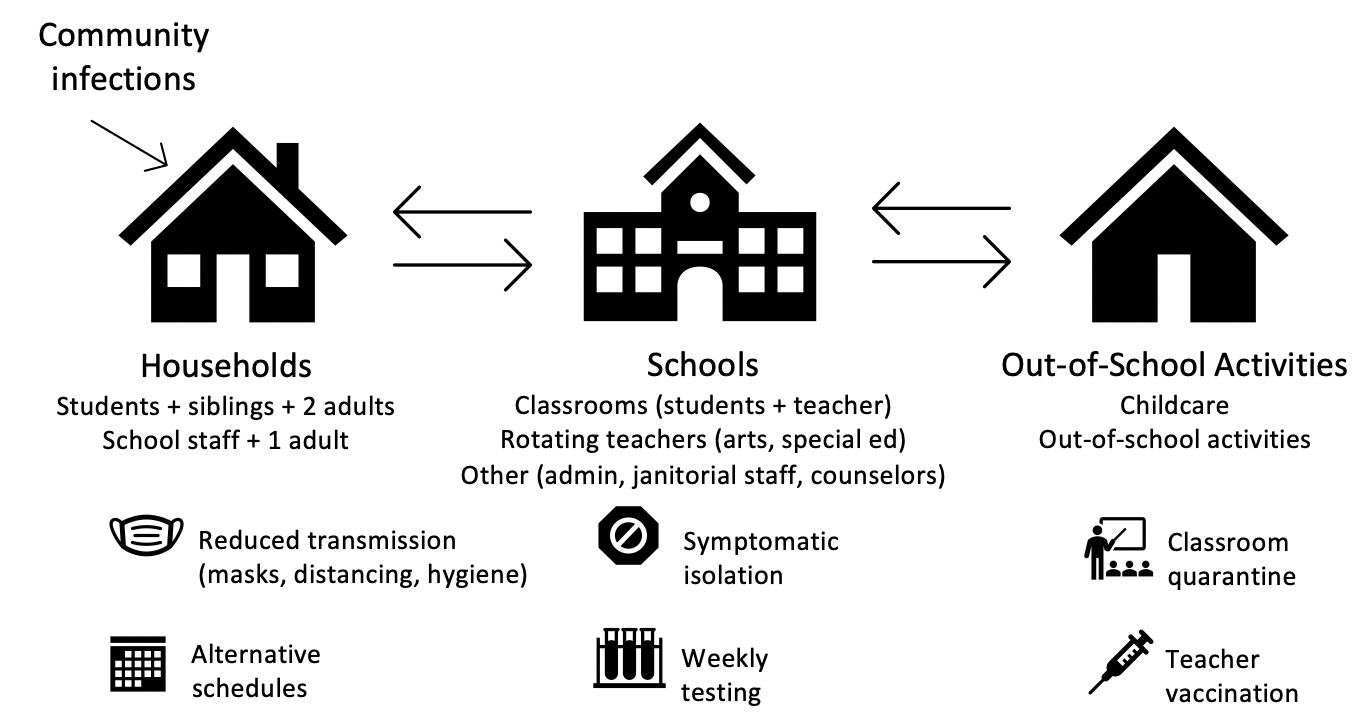
\includegraphics[width=150mm]{model2.png}
\caption{\label{fig1}Model diagram.  The model includes 3 primary domains: households, schools, and out-of-school social/childcare mixing and incorporates a range of interventions to prevent or reduce transmission.}
\end{figure}

\clearpage

\begin{longtable}[]{@{}lll@{}}
\caption{Parameter values. \label{tab:tbl1}}\tabularnewline
\toprule
\begin{minipage}[b]{0.28\columnwidth}\raggedright
Parameter\strut
\end{minipage} & \begin{minipage}[b]{0.09\columnwidth}\raggedright
Value\strut
\end{minipage} & \begin{minipage}[b]{0.54\columnwidth}\raggedright
Source\strut
\end{minipage}\tabularnewline
\midrule
\endfirsthead
\toprule
\begin{minipage}[b]{0.28\columnwidth}\raggedright
Parameter\strut
\end{minipage} & \begin{minipage}[b]{0.09\columnwidth}\raggedright
Value\strut
\end{minipage} & \begin{minipage}[b]{0.54\columnwidth}\raggedright
Source\strut
\end{minipage}\tabularnewline
\midrule
\endhead
\begin{minipage}[t]{0.28\columnwidth}\raggedright
Number of students in elementary school\strut
\end{minipage} & \begin{minipage}[t]{0.09\columnwidth}\raggedright
638\strut
\end{minipage} & \begin{minipage}[t]{0.54\columnwidth}\raggedright
(\protect\hyperlink{ref-noauthor_digest_nodate}{37})\strut
\end{minipage}\tabularnewline
\begin{minipage}[t]{0.28\columnwidth}\raggedright
Average of students per elementary school class\strut
\end{minipage} & \begin{minipage}[t]{0.09\columnwidth}\raggedright
21.3\strut
\end{minipage} & \begin{minipage}[t]{0.54\columnwidth}\raggedright
Consistent with (\protect\hyperlink{ref-noauthor_digest_nodate}{37}), 5
classes per grade\strut
\end{minipage}\tabularnewline
\begin{minipage}[t]{0.28\columnwidth}\raggedright
Number of adults who are not primary teachers in elementary
schools\strut
\end{minipage} & \begin{minipage}[t]{0.09\columnwidth}\raggedright
30\strut
\end{minipage} & \begin{minipage}[t]{0.54\columnwidth}\raggedright
Estimate via school websites \& personal communication\strut
\end{minipage}\tabularnewline
\begin{minipage}[t]{0.28\columnwidth}\raggedright
Number of students in high school\strut
\end{minipage} & \begin{minipage}[t]{0.09\columnwidth}\raggedright
1451\strut
\end{minipage} & \begin{minipage}[t]{0.54\columnwidth}\raggedright
(\protect\hyperlink{ref-noauthor_digest_nodate}{37})\strut
\end{minipage}\tabularnewline
\begin{minipage}[t]{0.28\columnwidth}\raggedright
Average of students per high school class\strut
\end{minipage} & \begin{minipage}[t]{0.09\columnwidth}\raggedright
23\strut
\end{minipage} & \begin{minipage}[t]{0.54\columnwidth}\raggedright
Consistent with (\protect\hyperlink{ref-noauthor_digest_nodate}{37}), 16
classes per grade\strut
\end{minipage}\tabularnewline
\begin{minipage}[t]{0.28\columnwidth}\raggedright
Number of adults who are not primary teachers in elementary
schools\strut
\end{minipage} & \begin{minipage}[t]{0.09\columnwidth}\raggedright
30\strut
\end{minipage} & \begin{minipage}[t]{0.54\columnwidth}\raggedright
Estimate via school websites \& personal communication\strut
\end{minipage}\tabularnewline
\begin{minipage}[t]{0.28\columnwidth}\raggedright
Probability of asymptomatic disease for adults\strut
\end{minipage} & \begin{minipage}[t]{0.09\columnwidth}\raggedright
0.2\strut
\end{minipage} & \begin{minipage}[t]{0.54\columnwidth}\raggedright
(\protect\hyperlink{ref-byambasuren_estimating_2020}{46})\strut
\end{minipage}\tabularnewline
\begin{minipage}[t]{0.28\columnwidth}\raggedright
Probability of asymptomatic disease for children\strut
\end{minipage} & \begin{minipage}[t]{0.09\columnwidth}\raggedright
0.4\strut
\end{minipage} & \begin{minipage}[t]{0.54\columnwidth}\raggedright
(\protect\hyperlink{ref-fontanet_sars-cov-2_2020}{8})\strut
\end{minipage}\tabularnewline
\begin{minipage}[t]{0.28\columnwidth}\raggedright
Relative infectiousness of asymptomatic disease\strut
\end{minipage} & \begin{minipage}[t]{0.09\columnwidth}\raggedright
0.5\strut
\end{minipage} & \begin{minipage}[t]{0.54\columnwidth}\raggedright
(\protect\hyperlink{ref-byambasuren_estimating_2020}{46})\strut
\end{minipage}\tabularnewline
\begin{minipage}[t]{0.28\columnwidth}\raggedright
Probability of subclinical disease for adults (includes
asymptomatic)\strut
\end{minipage} & \begin{minipage}[t]{0.09\columnwidth}\raggedright
0.4\strut
\end{minipage} & \begin{minipage}[t]{0.54\columnwidth}\raggedright
\strut
\end{minipage}\tabularnewline
\begin{minipage}[t]{0.28\columnwidth}\raggedright
Probability of subclinical disease for children (includes
asymptomatic)\strut
\end{minipage} & \begin{minipage}[t]{0.09\columnwidth}\raggedright
0.8\strut
\end{minipage} & \begin{minipage}[t]{0.54\columnwidth}\raggedright
(\protect\hyperlink{ref-han_clinical_2020}{60})\strut
\end{minipage}\tabularnewline
\begin{minipage}[t]{0.28\columnwidth}\raggedright
Household attack rate\strut
\end{minipage} & \begin{minipage}[t]{0.09\columnwidth}\raggedright
20\% (\textasciitilde4\% per day)\strut
\end{minipage} & \begin{minipage}[t]{0.54\columnwidth}\raggedright
(\protect\hyperlink{ref-madewell_household_2020}{38})\strut
\end{minipage}\tabularnewline
\begin{minipage}[t]{0.28\columnwidth}\raggedright
Classroom attack rate\strut
\end{minipage} & \begin{minipage}[t]{0.09\columnwidth}\raggedright
1/2/3\% per day\strut
\end{minipage} & \begin{minipage}[t]{0.54\columnwidth}\raggedright
\strut
\end{minipage}\tabularnewline
\begin{minipage}[t]{0.28\columnwidth}\raggedright
Relative attack rate for random school contacts (vs.~classroom)\strut
\end{minipage} & \begin{minipage}[t]{0.09\columnwidth}\raggedright
0.13\strut
\end{minipage} & \begin{minipage}[t]{0.54\columnwidth}\raggedright
Approximately 45 minutes\strut
\end{minipage}\tabularnewline
\begin{minipage}[t]{0.28\columnwidth}\raggedright
Relative attack rate for random staff contacts (vs.~classroom)\strut
\end{minipage} & \begin{minipage}[t]{0.09\columnwidth}\raggedright
2\strut
\end{minipage} & \begin{minipage}[t]{0.54\columnwidth}\raggedright
\strut
\end{minipage}\tabularnewline
\begin{minipage}[t]{0.28\columnwidth}\raggedright
Relative attack rate for childcare contacts (vs.~classroom)\strut
\end{minipage} & \begin{minipage}[t]{0.09\columnwidth}\raggedright
2\strut
\end{minipage} & \begin{minipage}[t]{0.54\columnwidth}\raggedright
Assuming fewer precautions\strut
\end{minipage}\tabularnewline
\begin{minipage}[t]{0.28\columnwidth}\raggedright
Distribution on viral load\strut
\end{minipage} & \begin{minipage}[t]{0.09\columnwidth}\raggedright
Lognormal (.84, .3)/.84\strut
\end{minipage} & \begin{minipage}[t]{0.54\columnwidth}\raggedright
Produces 20\%/45\% from differences in viral load
(\protect\hyperlink{ref-kerr_covasim_2020}{47})\strut
\end{minipage}\tabularnewline
\begin{minipage}[t]{0.28\columnwidth}\raggedright
Incubation period (from exposure to symptoms, if symptomatic)\strut
\end{minipage} & \begin{minipage}[t]{0.09\columnwidth}\raggedright
Gamma (5.8, 0.95)\strut
\end{minipage} & \begin{minipage}[t]{0.54\columnwidth}\raggedright
Estimated from (\protect\hyperlink{ref-lauer_incubation_2020}{61})\strut
\end{minipage}\tabularnewline
\begin{minipage}[t]{0.28\columnwidth}\raggedright
Start of infectiousness relative to symptoms\strut
\end{minipage} & \begin{minipage}[t]{0.09\columnwidth}\raggedright
Normal (1.2, 0.4)\strut
\end{minipage} & \begin{minipage}[t]{0.54\columnwidth}\raggedright
Estimated as mean 1.3 days,
(\protect\hyperlink{ref-gatto_spread_2020}{63}) mean 1.2 days w/lower
bound of 95\% CI of 3 for start and 2 for peak
(\protect\hyperlink{ref-he_temporal_2020}{64})\strut
\end{minipage}\tabularnewline
\begin{minipage}[t]{0.28\columnwidth}\raggedright
Duration of infectiousness\strut
\end{minipage} & \begin{minipage}[t]{0.09\columnwidth}\raggedright
Lognormal (5, 2)\strut
\end{minipage} & \begin{minipage}[t]{0.54\columnwidth}\raggedright
(\protect\hyperlink{ref-kerr_covasim_2020}{47})\strut
\end{minipage}\tabularnewline
\begin{minipage}[t]{0.28\columnwidth}\raggedright
Duration of isolation and quarantine\strut
\end{minipage} & \begin{minipage}[t]{0.09\columnwidth}\raggedright
10 days\strut
\end{minipage} & \begin{minipage}[t]{0.54\columnwidth}\raggedright
(\protect\hyperlink{ref-cdc_covid-19_2020}{32})\strut
\end{minipage}\tabularnewline
\begin{minipage}[t]{0.28\columnwidth}\raggedright
Teacher vaccination uptake\strut
\end{minipage} & \begin{minipage}[t]{0.09\columnwidth}\raggedright
75\%\strut
\end{minipage} & \begin{minipage}[t]{0.54\columnwidth}\raggedright
(\protect\hyperlink{ref-noauthor_map_2020}{1},\protect\hyperlink{ref-gallup_inc_willingness_2020}{33})\strut
\end{minipage}\tabularnewline
\begin{minipage}[t]{0.28\columnwidth}\raggedright
Vaccination effectiveness\strut
\end{minipage} & \begin{minipage}[t]{0.09\columnwidth}\raggedright
90\%\strut
\end{minipage} & \begin{minipage}[t]{0.54\columnwidth}\raggedright
(\protect\hyperlink{ref-polack_safety_2020}{35}), assuming that vaccine
blocks infections as well as prevents symptomatic illness (currently
unknown)\strut
\end{minipage}\tabularnewline
\begin{minipage}[t]{0.28\columnwidth}\raggedright
Test uptake\strut
\end{minipage} & \begin{minipage}[t]{0.09\columnwidth}\raggedright
90\%\strut
\end{minipage} & \begin{minipage}[t]{0.54\columnwidth}\raggedright
Assumed\strut
\end{minipage}\tabularnewline
\begin{minipage}[t]{0.28\columnwidth}\raggedright
Test sensitivity during infectious period\strut
\end{minipage} & \begin{minipage}[t]{0.09\columnwidth}\raggedright
90\%\strut
\end{minipage} & \begin{minipage}[t]{0.54\columnwidth}\raggedright
\strut
\end{minipage}\tabularnewline
\bottomrule
\end{longtable}

\clearpage

\blandscape

\begin{figure}
\centering
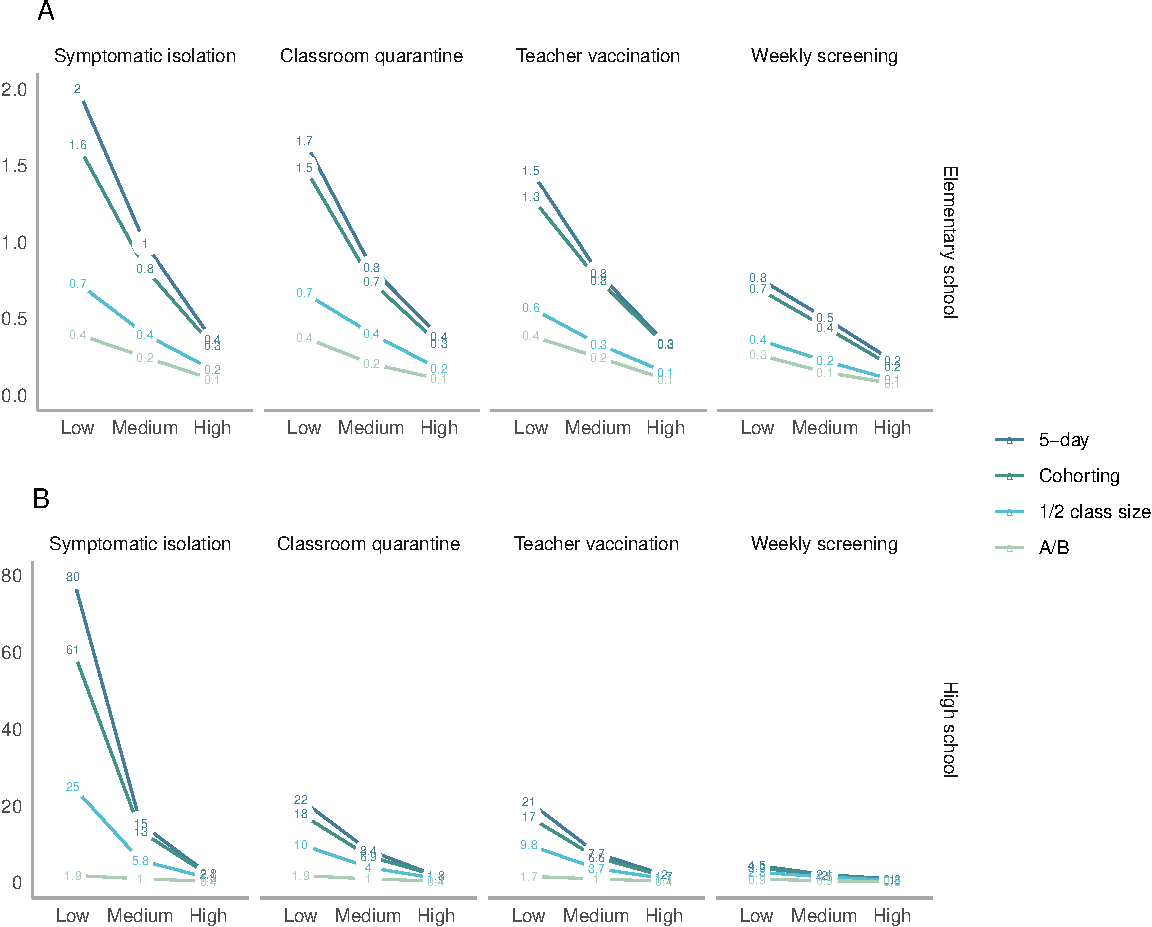
\includegraphics{Schools_draft_files/figure-latex/fig2-1.pdf}
\caption{\label{fig2} Average number of total secondary transmissions
over 30 days (outside of the index case's household) following a single
introduction into a school community. (This is not an estimate of R, the
effective reproduction number, which is displayed in Figure \ref{figr}.)
These include both transmission directly from the index case, as well as
from secondary and tertiary cases. The top panel shows elementary
schools, where children are assumed to be less susceptible and less
infectious, while the bottom panel shows high schools. Note that axes
differ across rows. The x-axes vary the level of prevention measure
uptake, with low uptake assuming minimal interventions and high uptake
assuming intensive interventions. Line colors correspond to scheduling
strategies.}
\end{figure}

\elandscape

\clearpage

\begin{figure}
\centering
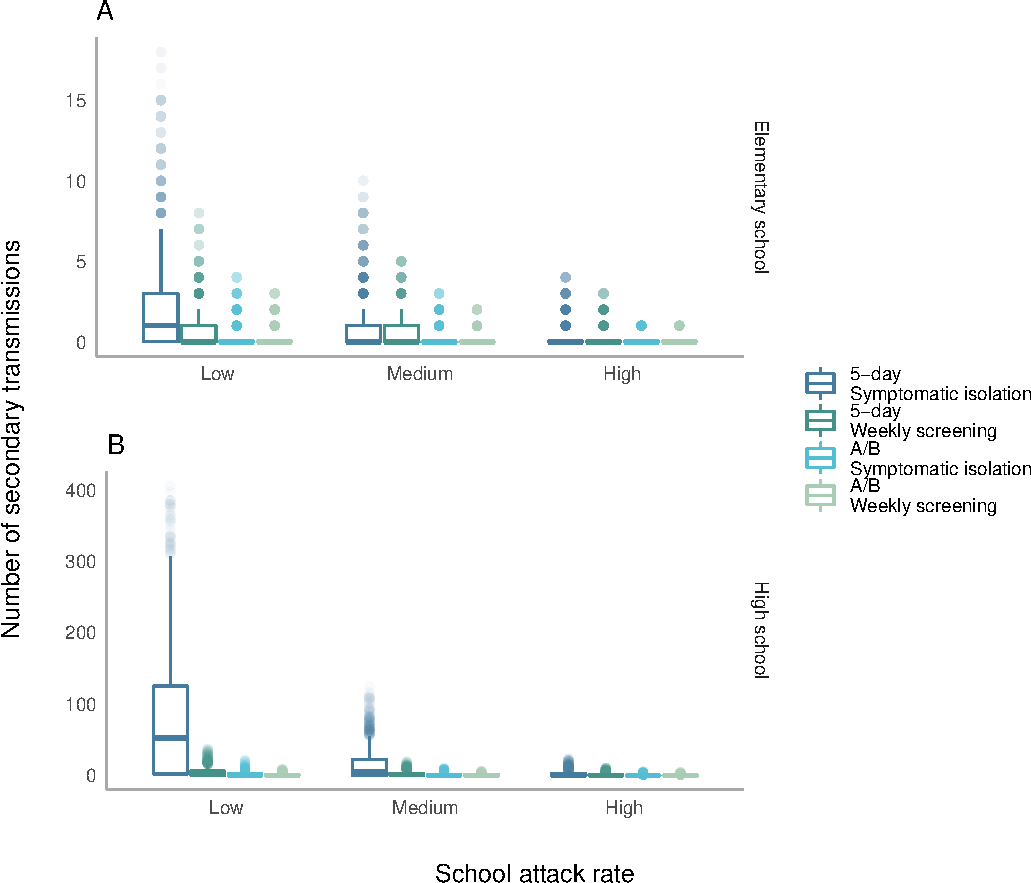
\includegraphics{Schools_draft_files/figure-latex/fig3.2-1.pdf}
\caption{\label{fig3} Distribution of secondary transmissions when a
single case is introduced. The y-axis displays the number of secondary
transmissions (outside of the index case's household) when a case is
introduced. Transmissions include both those directly from the index
case, as well as those from secondary and tertiary cases. Distributions
are truncated at the 99.5th quantile, i.e.~all outcomes occur with at
least probability 1/200.}
\end{figure}

\blandscape

\begin{figure}
\centering
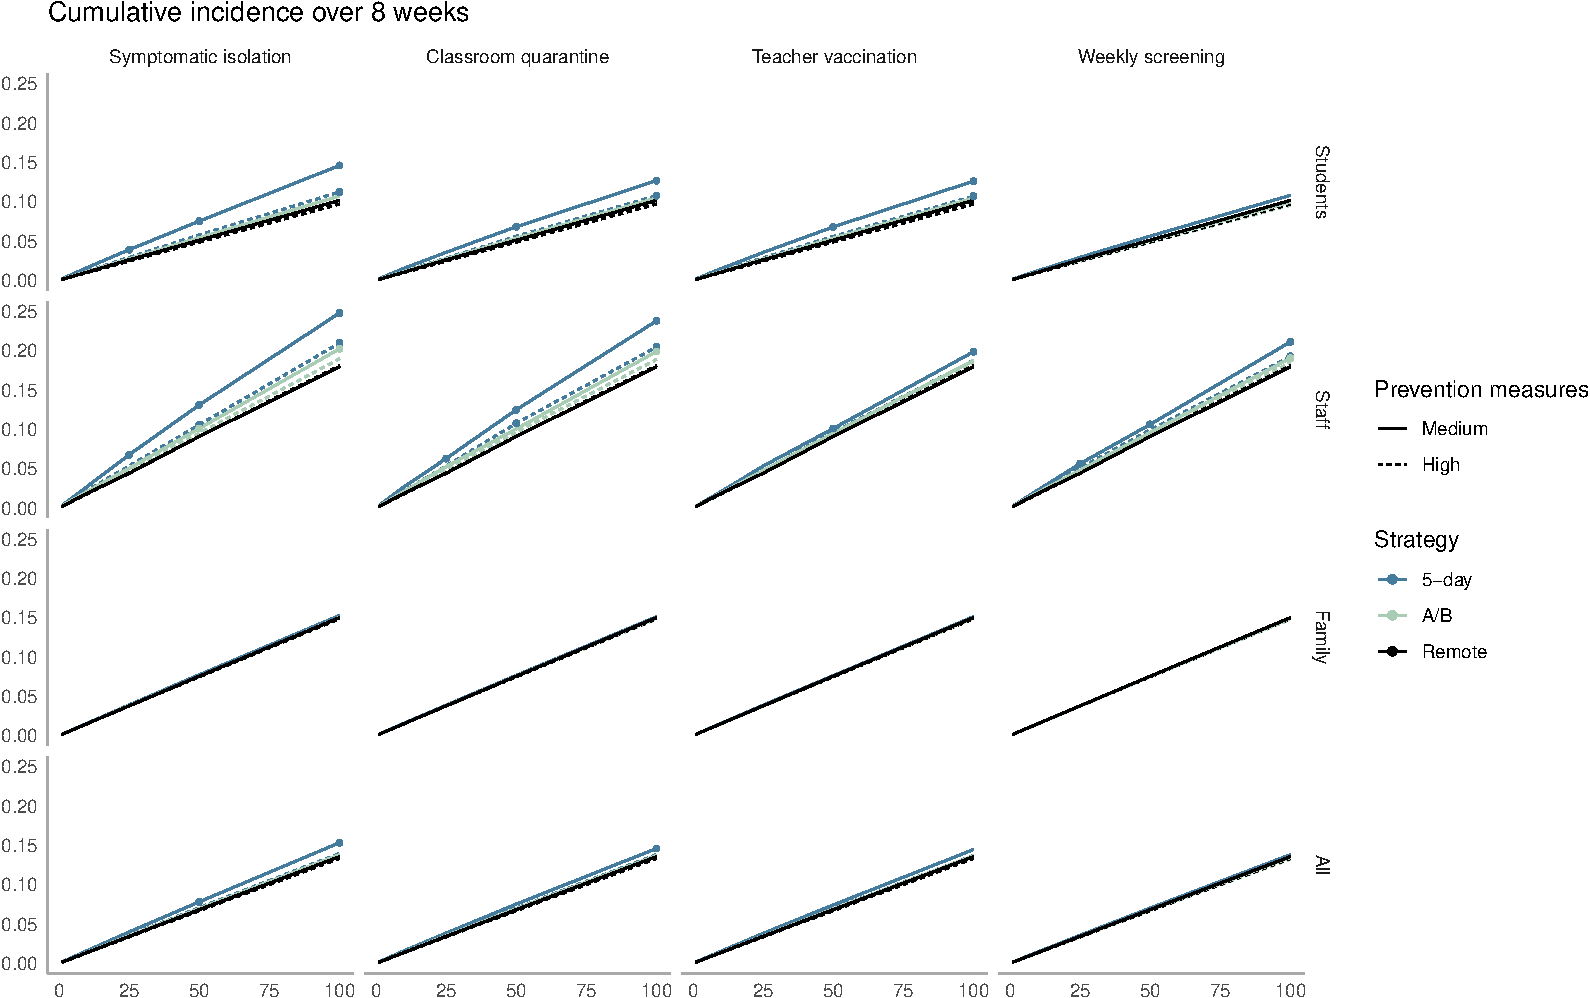
\includegraphics{Schools_draft_files/figure-latex/unnamed-chunk-1-1.pdf}
\caption{\label{fig4} Cumulative incidence over 8 weeks in elementary
schools. The x-axis shows the average daily community incidence per
100,000 population. The y-axis shows cumulative incidence over 8 weeks.
Columns denote different isolation, quarantine, vaccination, and
detection strategies, while rows show different population subgroups.
Points are marked for strategies with increased incidence over remote
learning that exceeds 1\%.}
\end{figure}

\elandscape

\blandscape

\begin{figure}
\centering
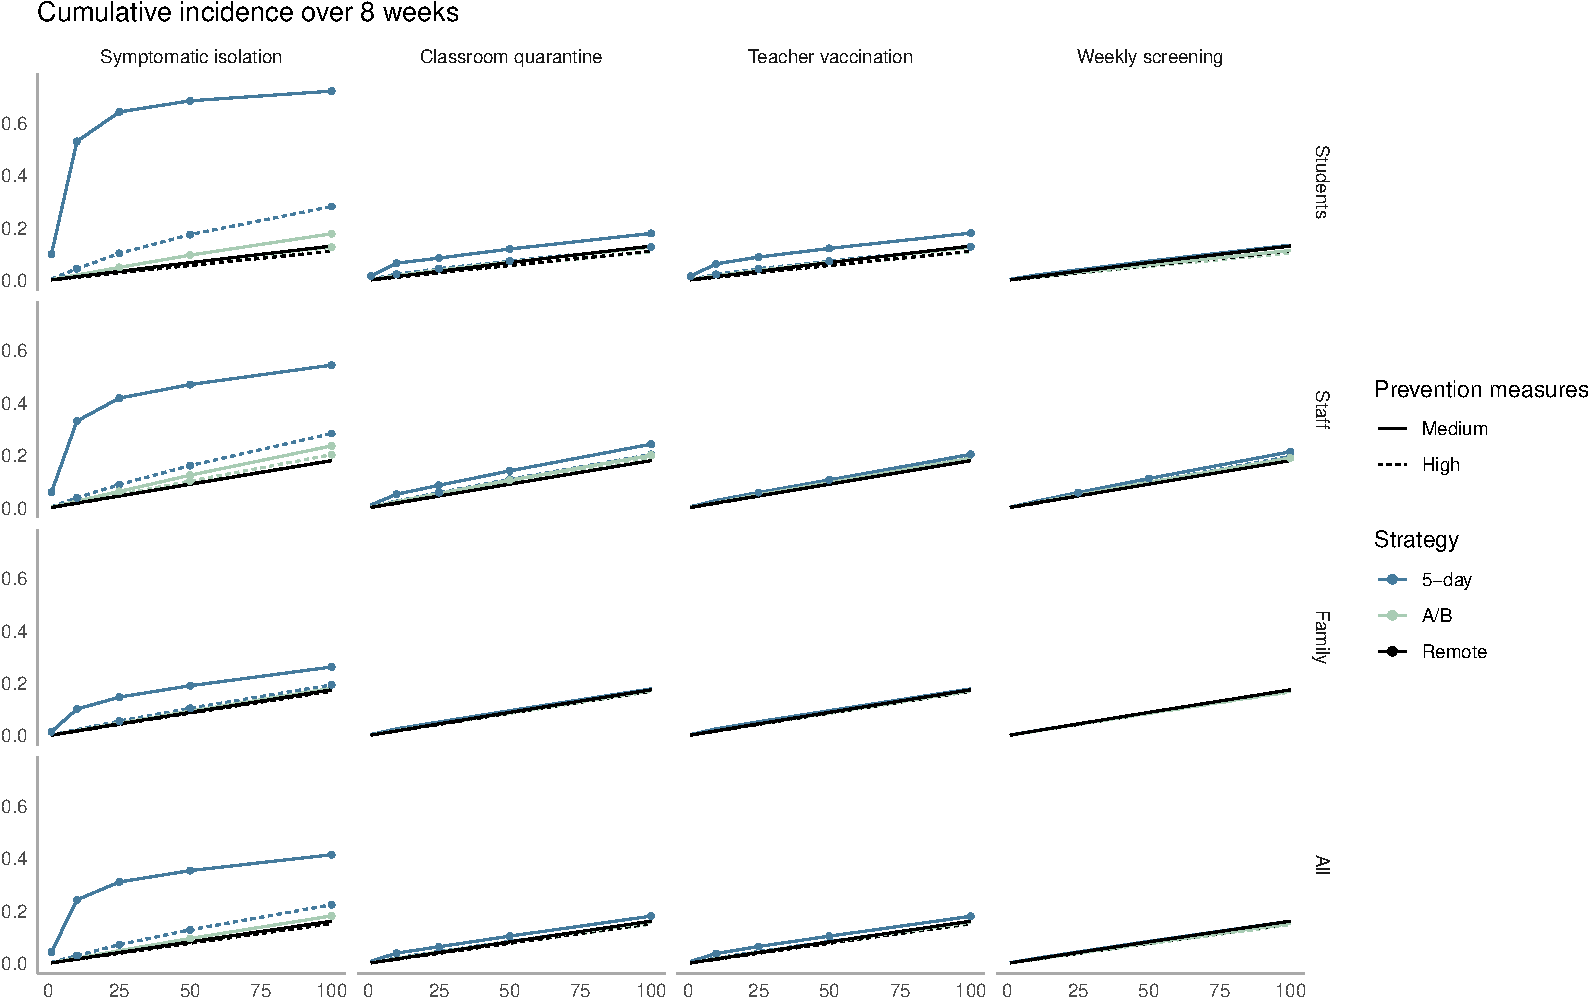
\includegraphics{Schools_draft_files/figure-latex/unnamed-chunk-2-1.pdf}
\caption{\label{fig5} Cumulative incidence over 8 weeks in high schools.
The x-axis shows the average daily community incidence per 100,000
population. The y-axis shows cumulative incidence over 8 weeks. Columns
denote different isolation, quarantine, vaccination, and detection
strategies, while rows show different population subgroups. Points are
marked for strategies with increased incidence over remote learning that
exceeds 1\%.}
\end{figure}

\elandscape

\hypertarget{supplement}{%
\section{Supplement}\label{supplement}}

\setcounter{figure}{0}
\renewcommand{\thesubsection}{\thesection.\arabic{subsection}}
\renewcommand{\thefigure}{S\arabic{figure}}

\begin{figure}
\centering
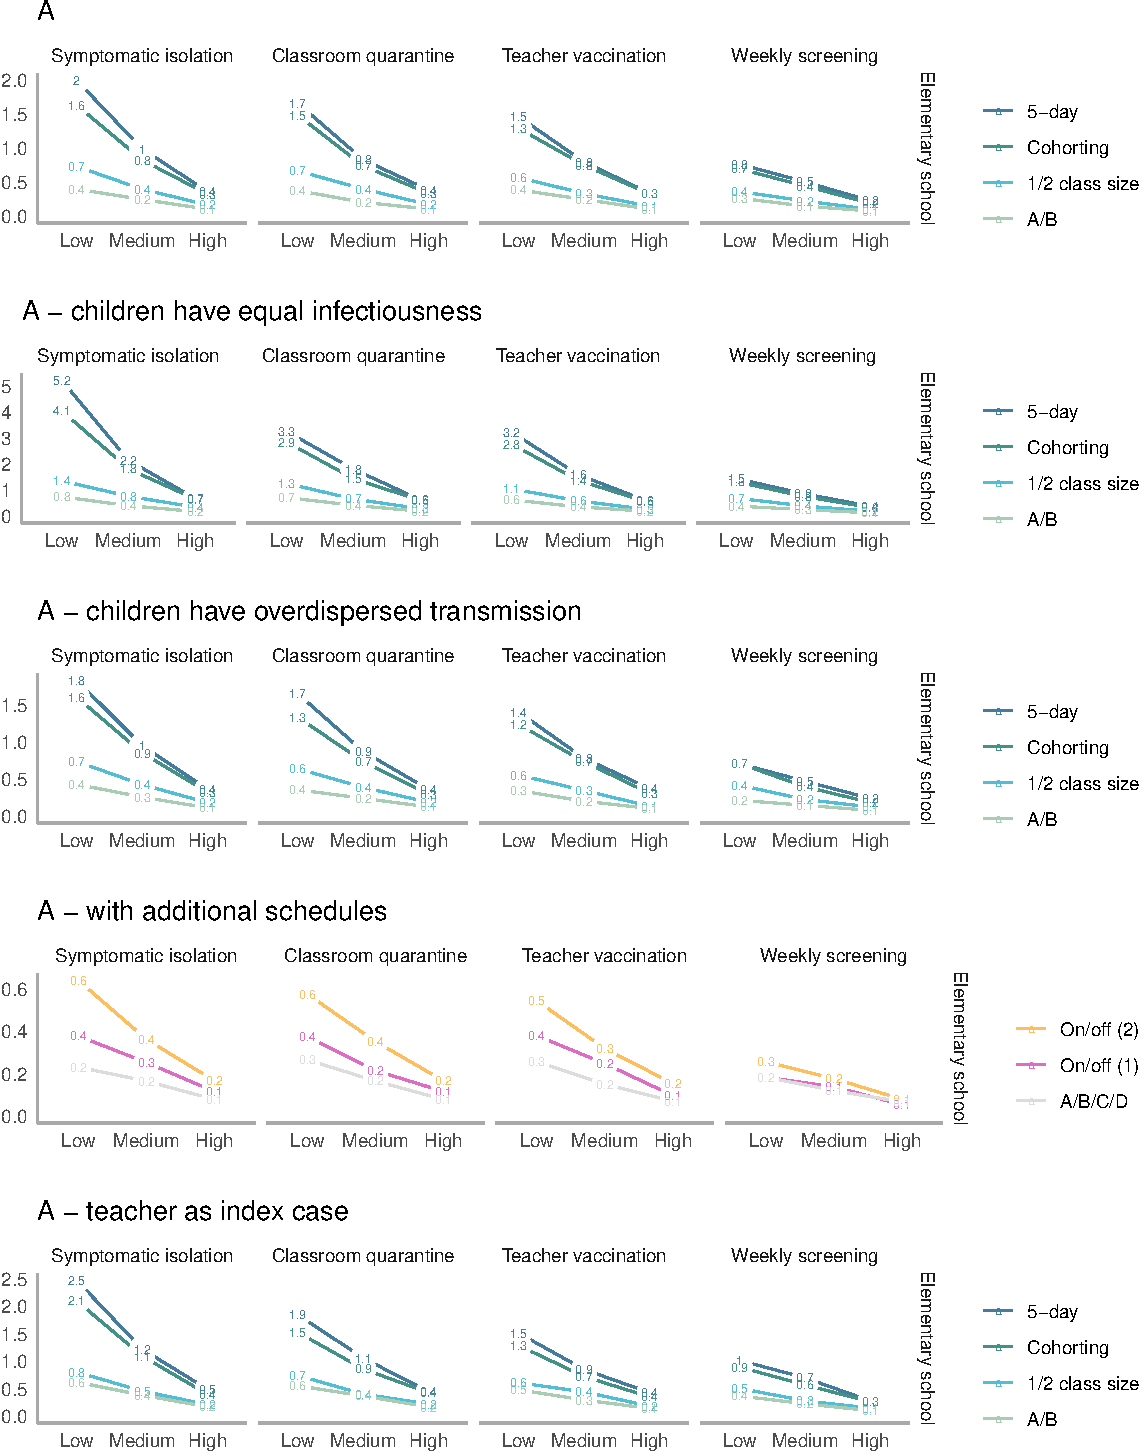
\includegraphics{Schools_draft_files/figure-latex/figs3-1.pdf}
\caption{\label{figs1} Sensitivity analyses (elementary schools) --
average number of total secondary transmissions over 30 days (outside of
the index case's household) following a single introduction into a
school community. The columns vary the level of prevention measure
uptake, with low uptake assuming minimal interventions and high uptake
assuming intensive interventions. Line colors correspond to scheduling
strategies.}
\end{figure}

\begin{figure}
\centering
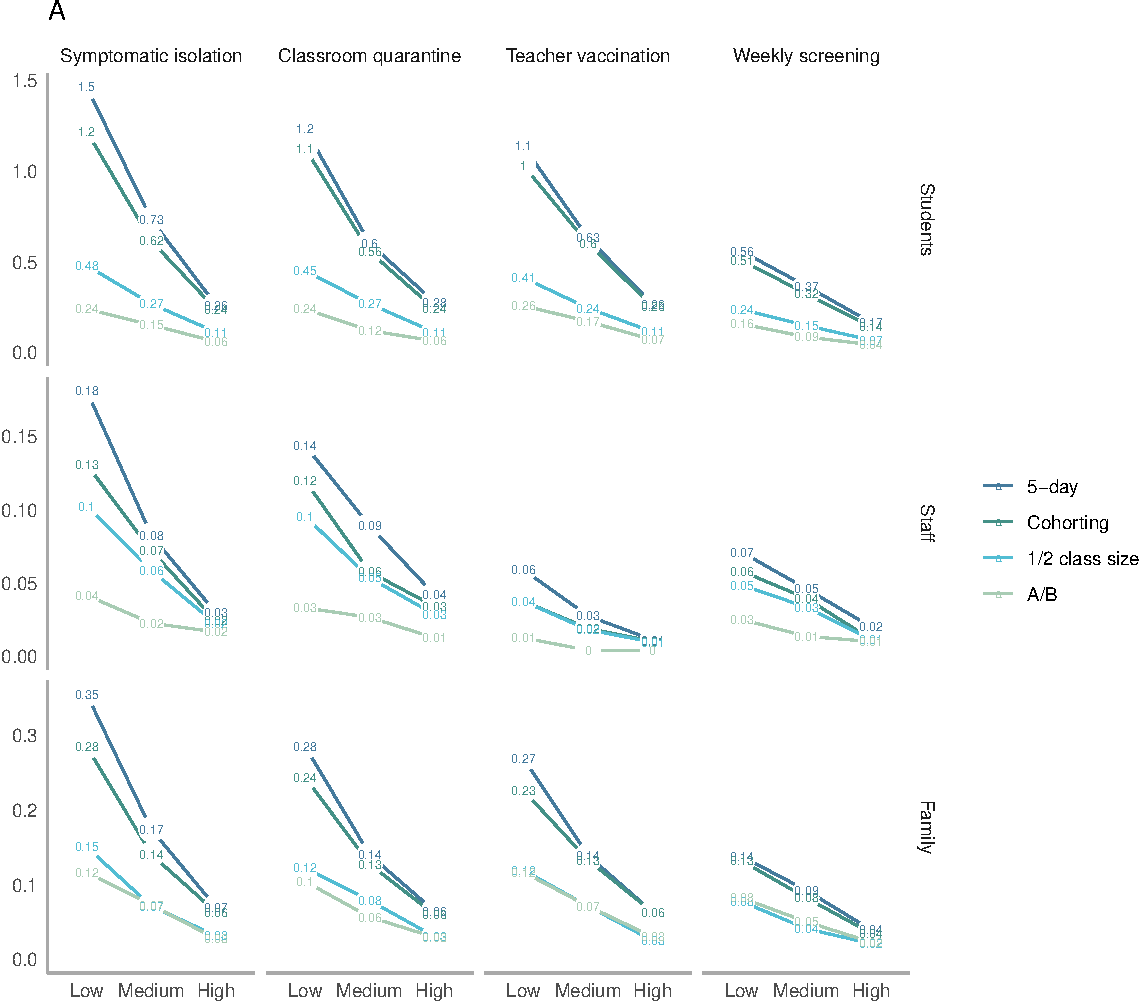
\includegraphics{Schools_draft_files/figure-latex/figs1-1.pdf}
\caption{\label{figs2} Sensitivity analysis - elementary schools by case
type. Average number of total secondary transmissions over 30 days
(outside of the index case's household) following a single introduction
into an elementary school community. These include both transmission
directly from the index case, as well as from secondary and tertiary
cases. The x-axes varies the level of prevention measure uptake, with
low uptake assuming minimal interventions and high uptake assuming
intensive interventions. Line colors correspond to scheduling
strategies.}
\end{figure}

\begin{figure}
\centering
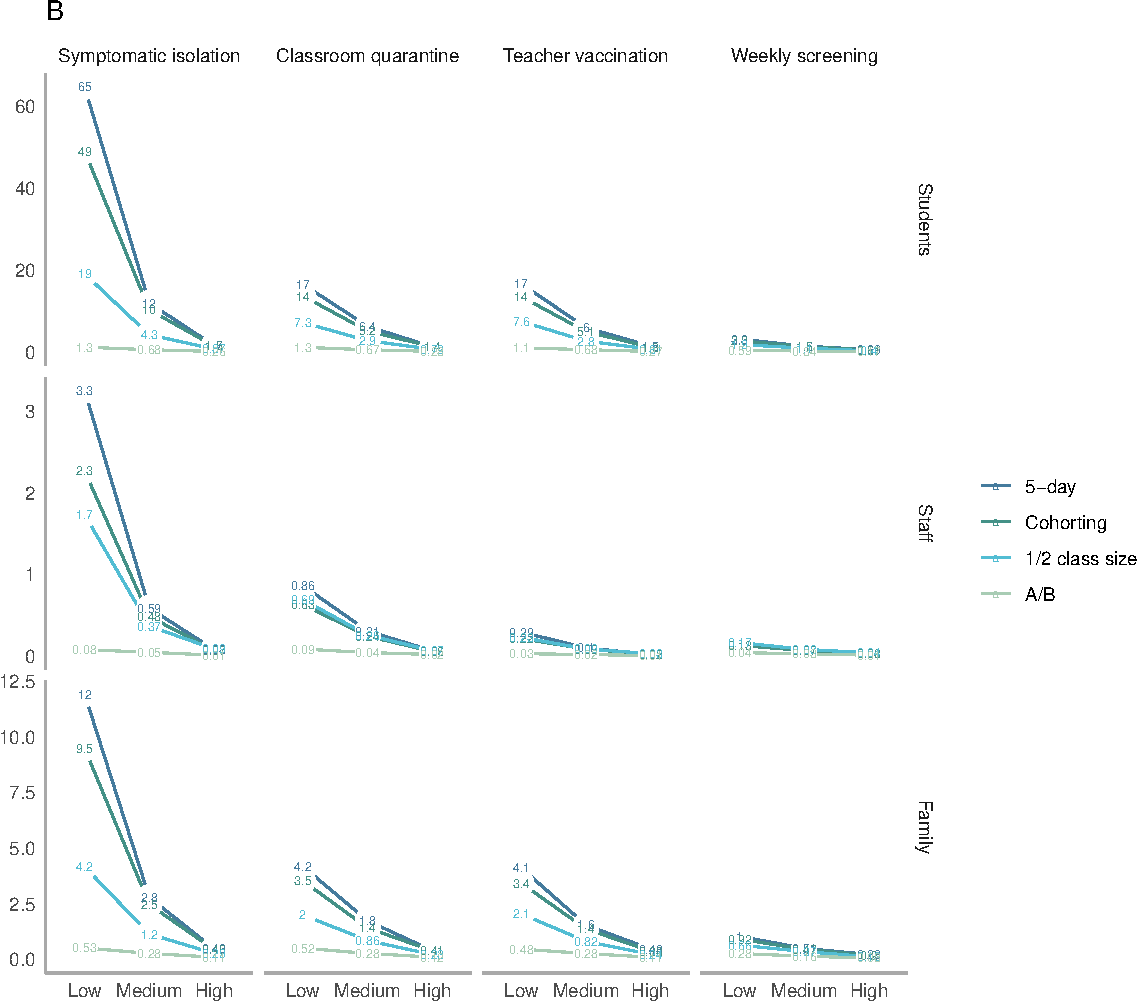
\includegraphics{Schools_draft_files/figure-latex/figs2-1.pdf}
\caption{\label{figs3} Sensitivity analysis - high schools by case type.
Average number of total secondary transmissions over 30 days (outside of
the index case's household) following a single introduction into an
elementary school community. These include both transmission directly
from the index case, as well as from secondary and tertiary cases. The
x-axes varies the level of prevention measure uptake, with low uptake
assuming minimal interventions and high uptake assuming intensive
interventions. Line colors correspond to scheduling strategies.}
\end{figure}

\begin{figure}
\centering
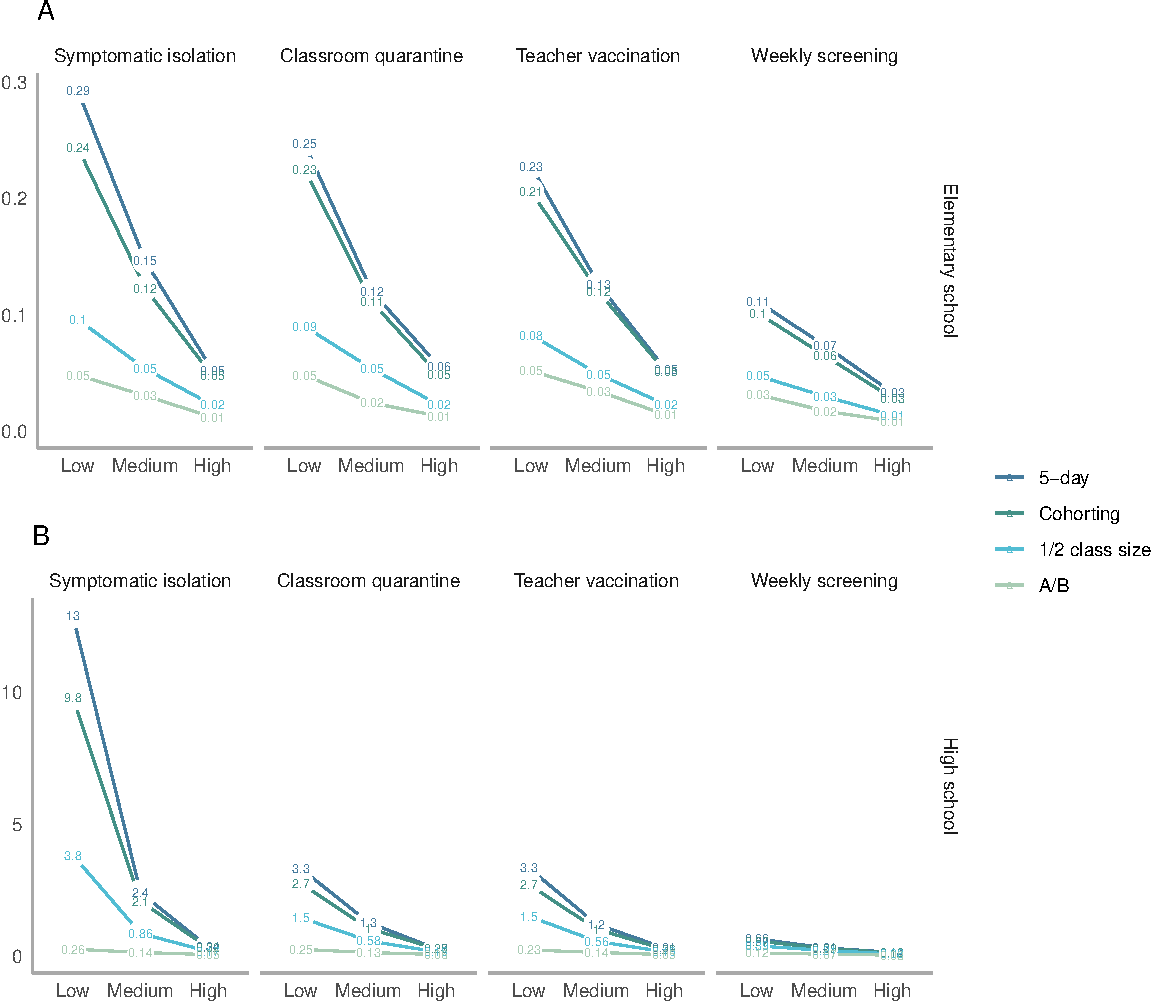
\includegraphics{Schools_draft_files/figure-latex/fign-1.pdf}
\caption{\label{figs4} Average number of clinically symptomatic cases in
staff and students over 30 days following a single introduction into a
school community. These include both transmission directly from the
index case, as well as from secondary and tertiary cases. The top panel
shows elementary schools, where children are assumed to be less
susceptible and less infectious, while the bottom panel shows high
schools. Note that axes differ across rows. The x-axes vary the level of
prevention measure uptake, with low uptake assuming minimal
interventions and high uptake assuming intensive interventions. Line
colors correspond to scheduling strategies.}
\end{figure}

\begin{figure}
\centering
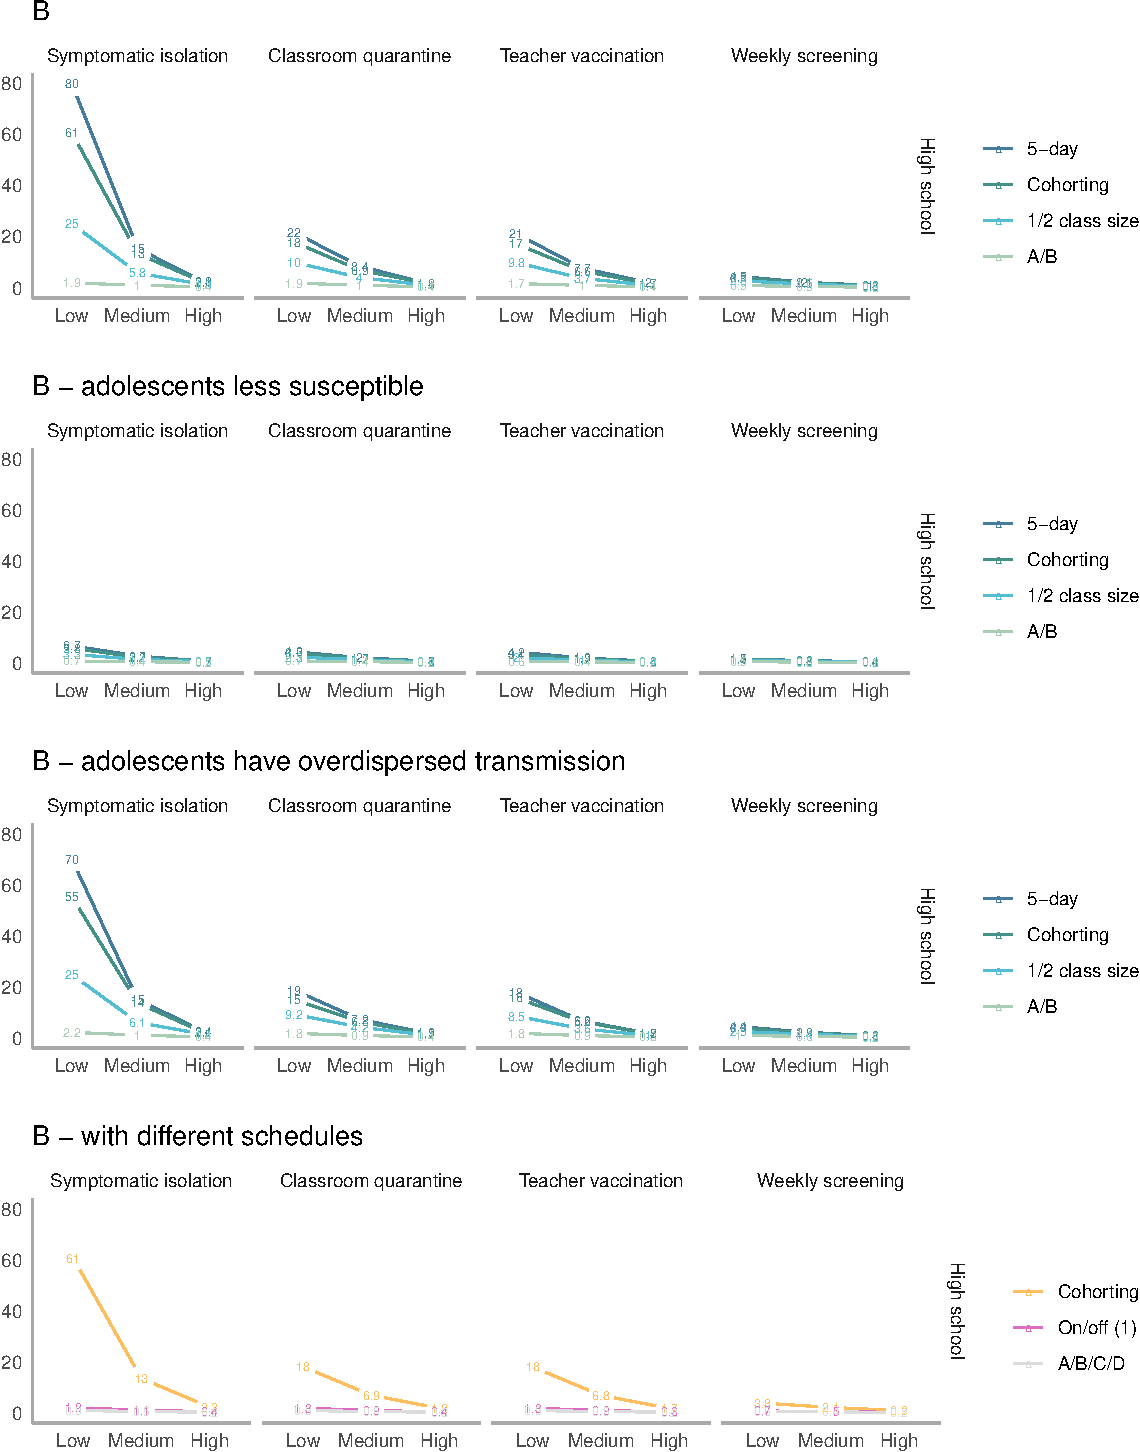
\includegraphics{Schools_draft_files/figure-latex/figs4-1.pdf}
\caption{\label{figs5} Sensitivity analyses (high schools) -- average
number of total secondary transmissions over 30 days (outside of the
index case's household) following a single introduction into a school
community. The columns vary the level of prevention measure uptake, with
low uptake assuming minimal interventions and high uptake assuming
intensive interventions. Line colors correspond to scheduling
strategies.}
\end{figure}

\blandscape

\begin{figure}
\centering
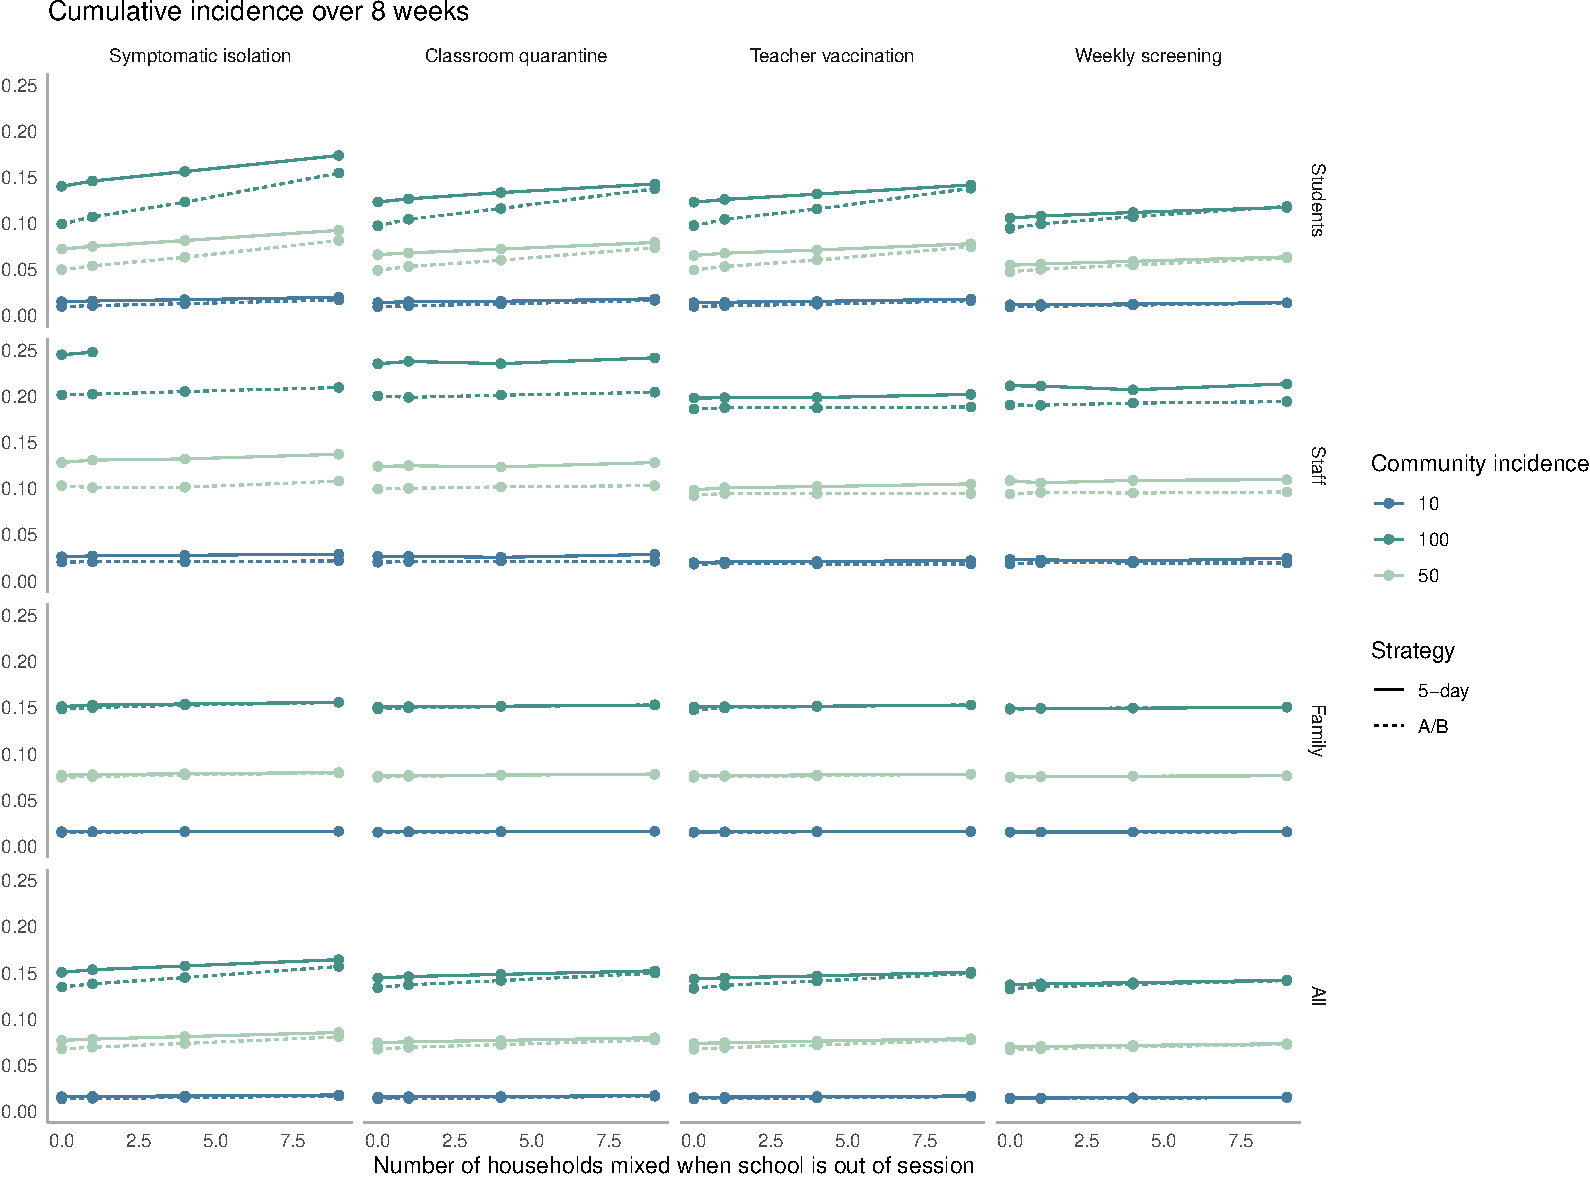
\includegraphics{Schools_draft_files/figure-latex/unnamed-chunk-3-1.pdf}
\caption{\label{figs6} Cumulative incidence over 8 weeks in elementary
schools across different levels of out-of-school mixing. The x-axis
shows the average daily community incidence per 100,000 population. The
y-axis shows cumulative incidence over 8 weeks. Columns denote different
isolation, quarantine, vaccination, and detection strategies, while rows
show different population subgroups.}
\end{figure}

\elandscape

\blandscape

\begin{figure}
\centering
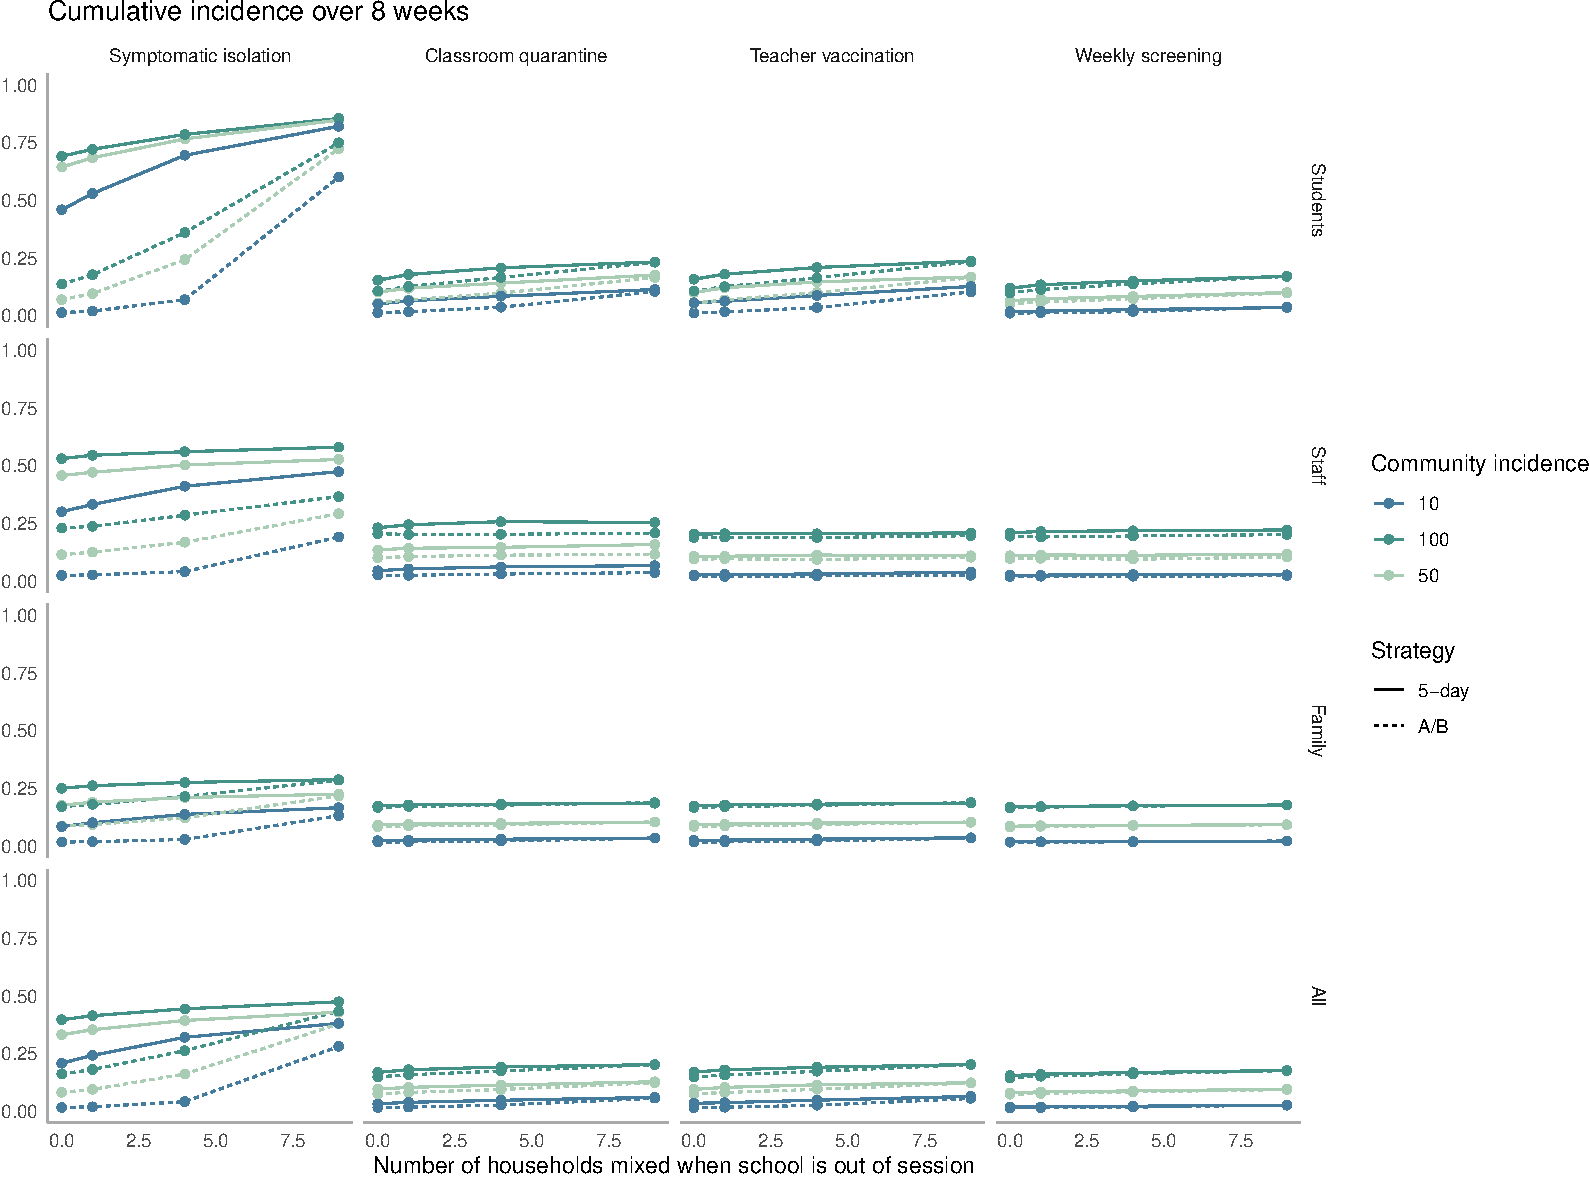
\includegraphics{Schools_draft_files/figure-latex/unnamed-chunk-4-1.pdf}
\caption{\label{figs7} Cumulative incidence over 8 weeks in high schools
across different levels of out-of-school mixing. The x-axis shows the
average daily community incidence per 100,000 population. The y-axis
shows cumulative incidence over 8 weeks. Columns denote different
isolation, quarantine, vaccination, and detection strategies, while rows
show different population subgroups.}
\end{figure}

\elandscape

\clearpage

\hypertarget{model}{%
\section{Model}\label{model}}

We use a Framework for Reconstructing Epidemiological Dynamics (FRED) to
generate household structures
(\protect\hyperlink{ref-wheaton_us_2014}{36}). For computational
simplicity, we used Maryland as a representative state, as sibling
structure (the main parameter of interest) did not appear sensitive to
location.

\begin{tabular}{cccc}
Maryland Elementary & Connecticut Elementary & Mississippi Elementary  & Texas Elementary  \\
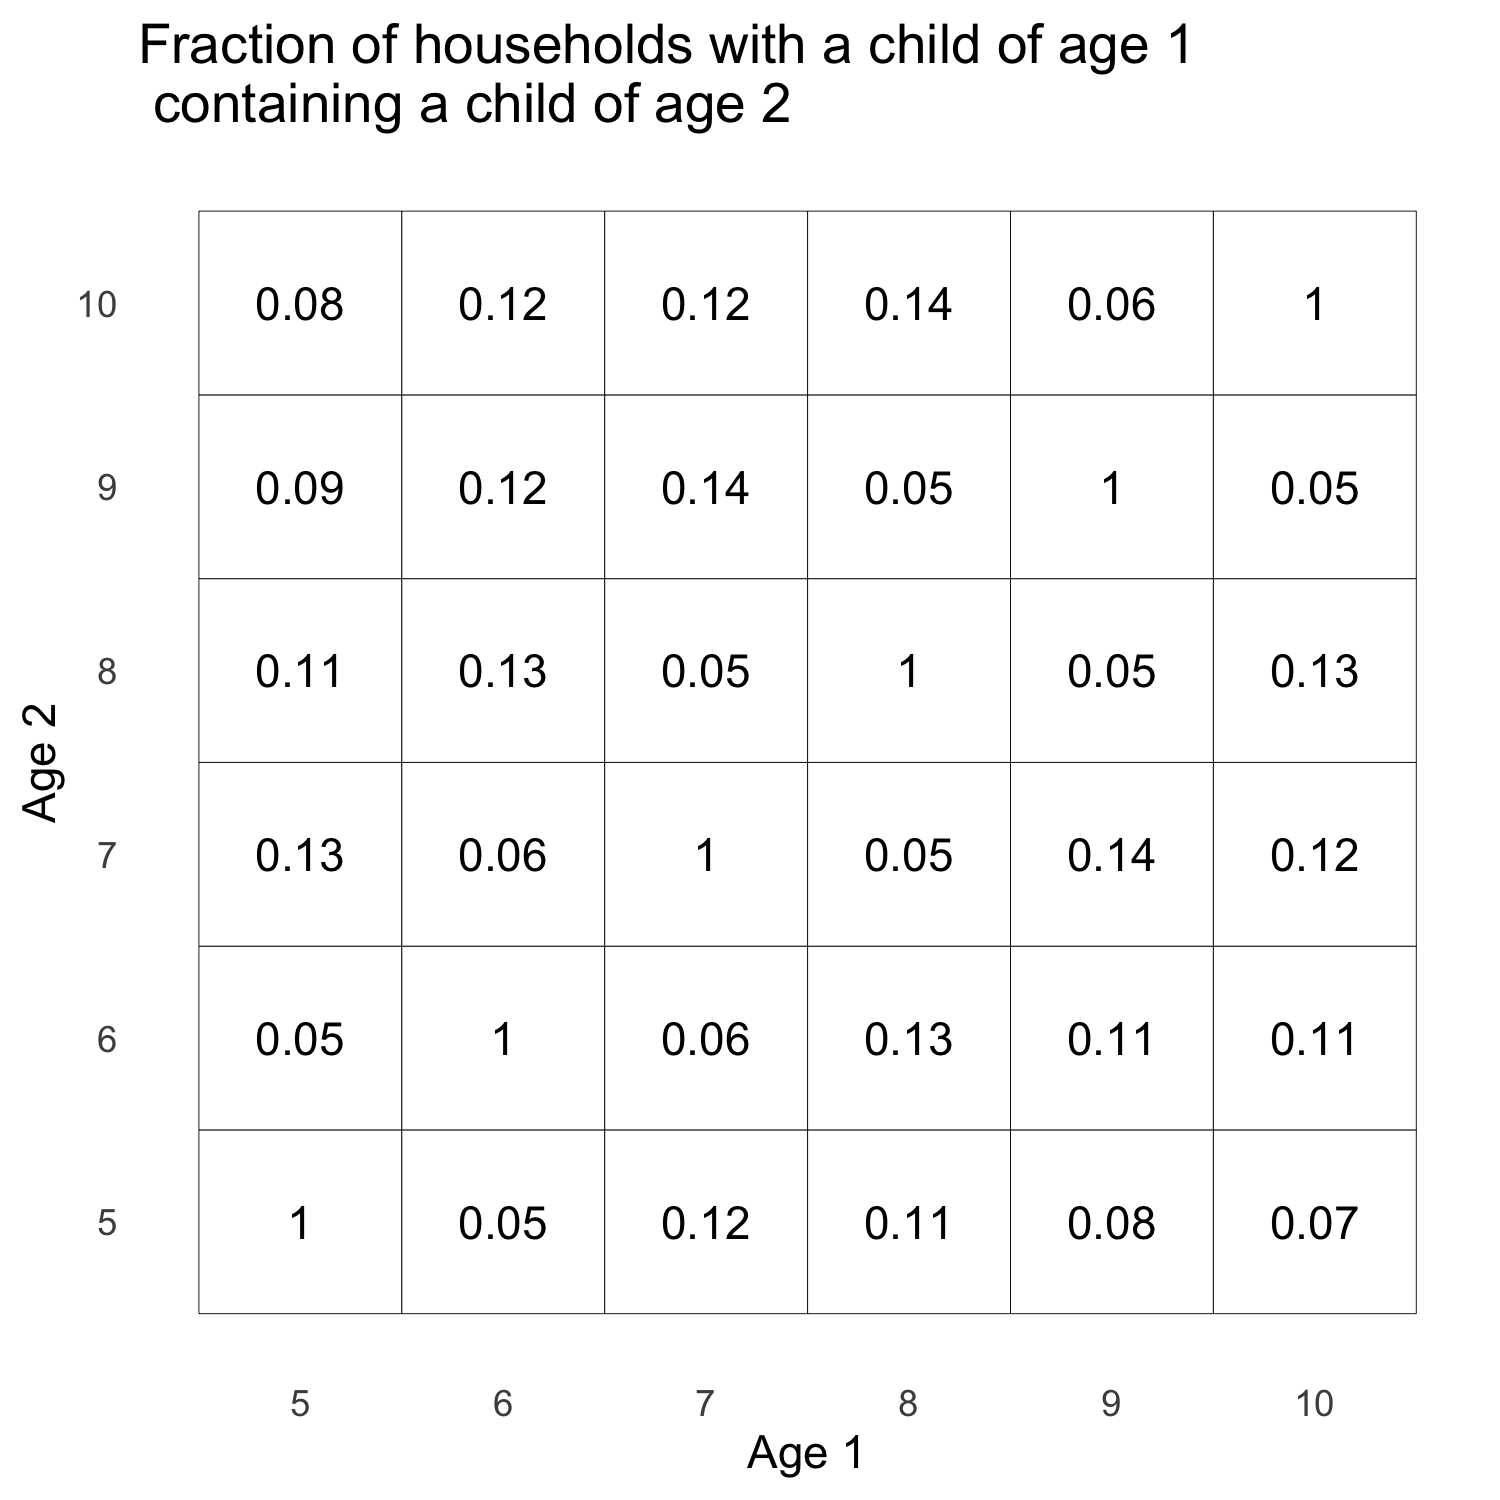
\includegraphics[width=40mm]{/Users/abilinski/Dropbox/Schools/Public code/0 - Synthetic Populations/2 - Output/sibling_heatmap_Maryland.png} &
      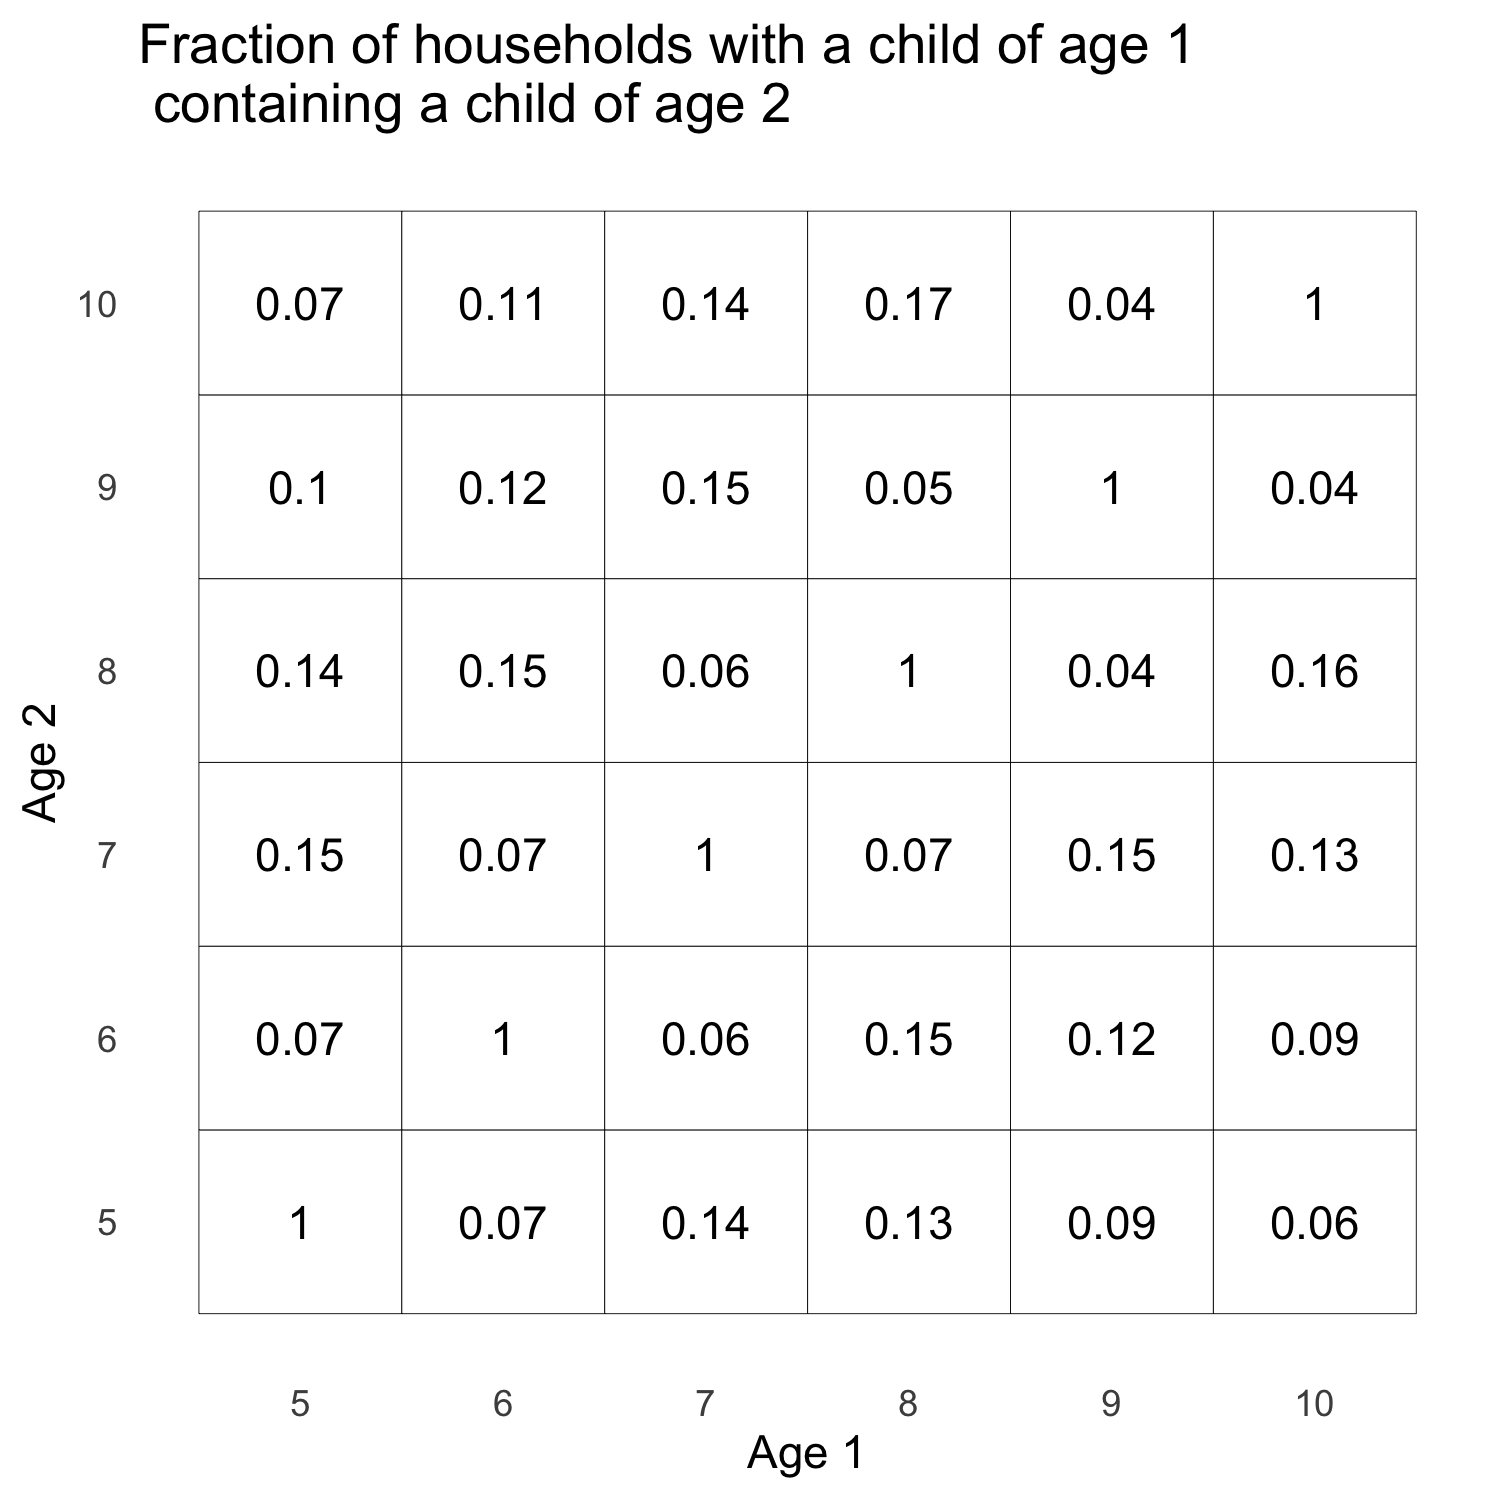
\includegraphics[width=40mm]{/Users/abilinski/Dropbox/Schools/Public code/0 - Synthetic Populations/2 - Output/sibling_heatmap_Connecticut.png} &
      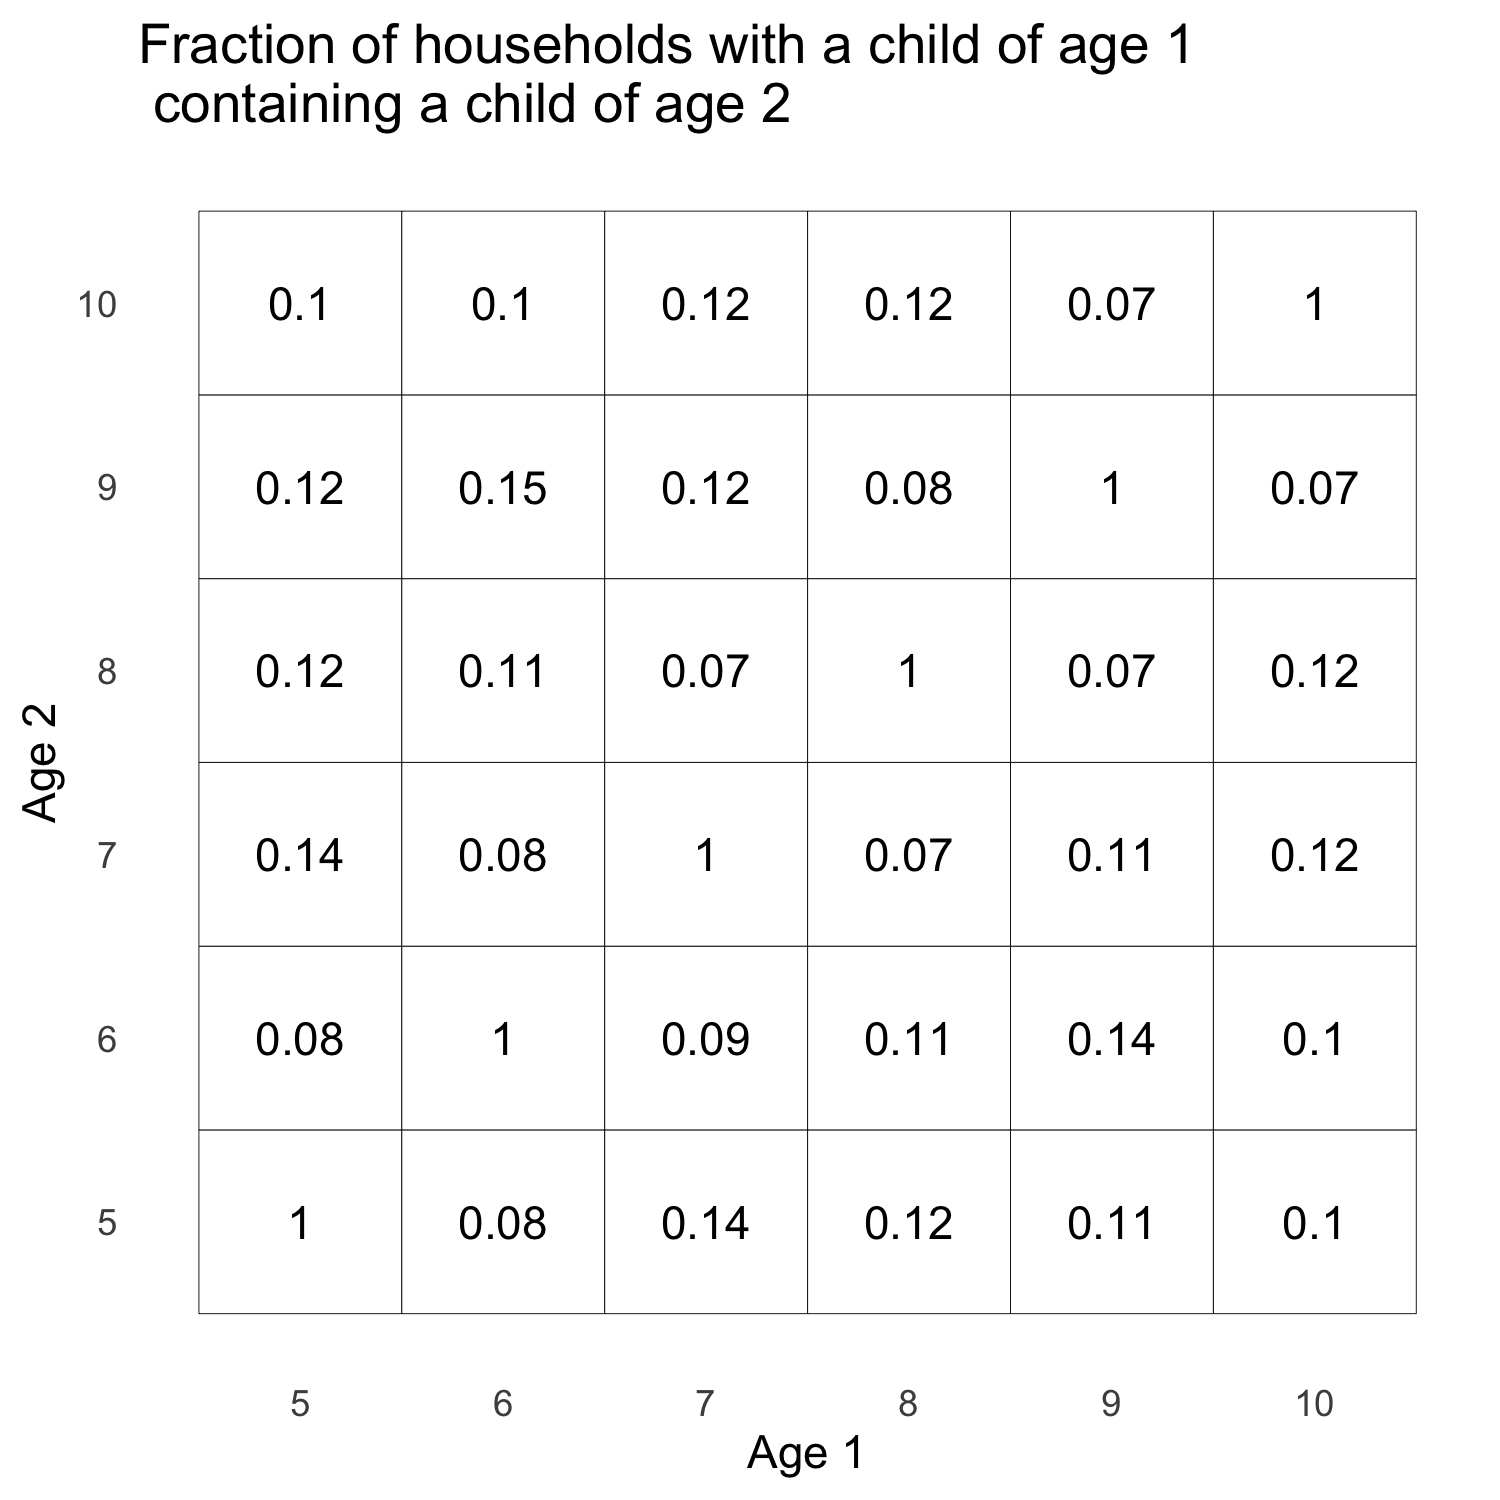
\includegraphics[width=40mm]{/Users/abilinski/Dropbox/Schools/Public code/0 - Synthetic Populations/2 - Output/sibling_heatmap_Mississippi.png} &
      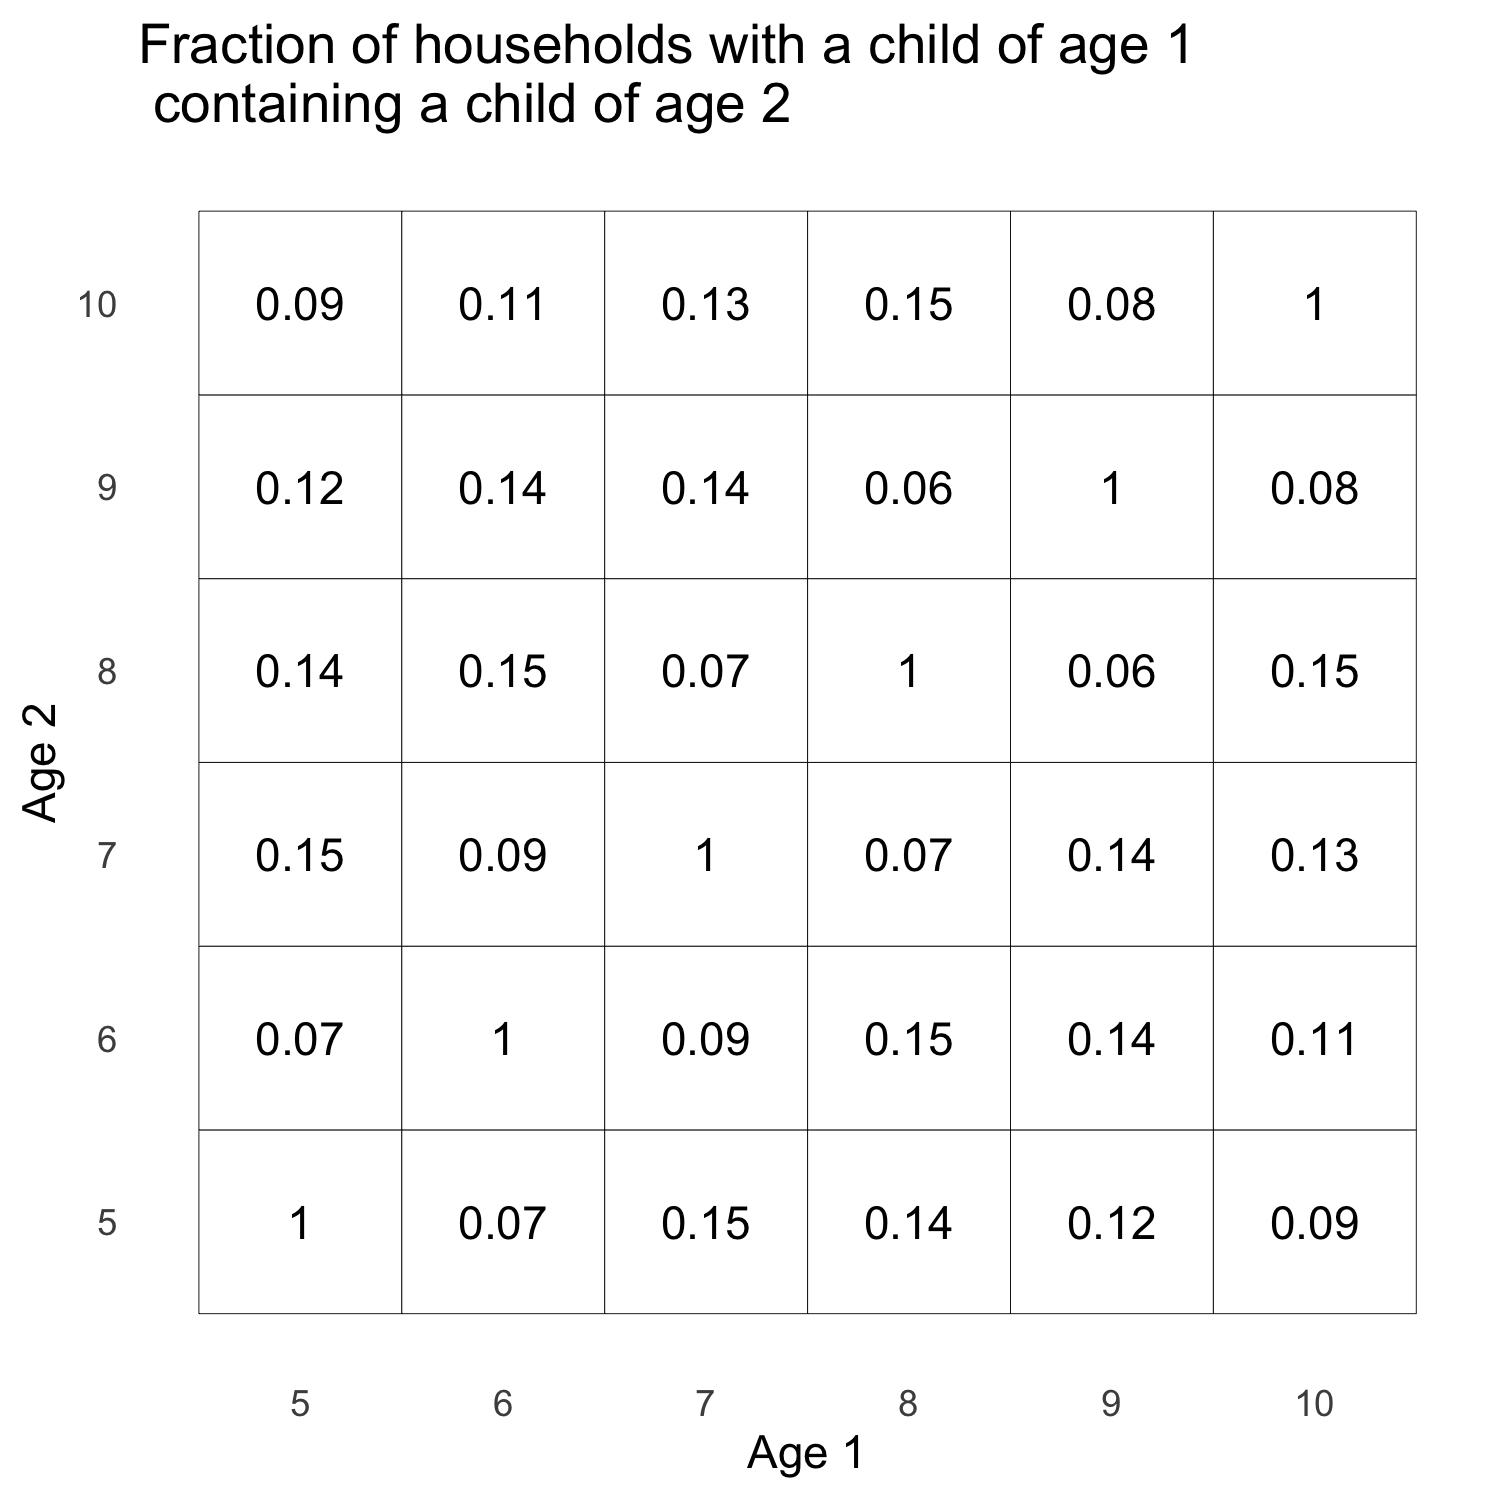
\includegraphics[width=40mm]{/Users/abilinski/Dropbox/Schools/Public code/0 - Synthetic Populations/2 - Output/sibling_heatmap_Texas.png} 
    \end{tabular}

\begin{tabular}{cccc}
Maryland HS & Connecticut HS & Mississippi HS  & Texas HS  \\
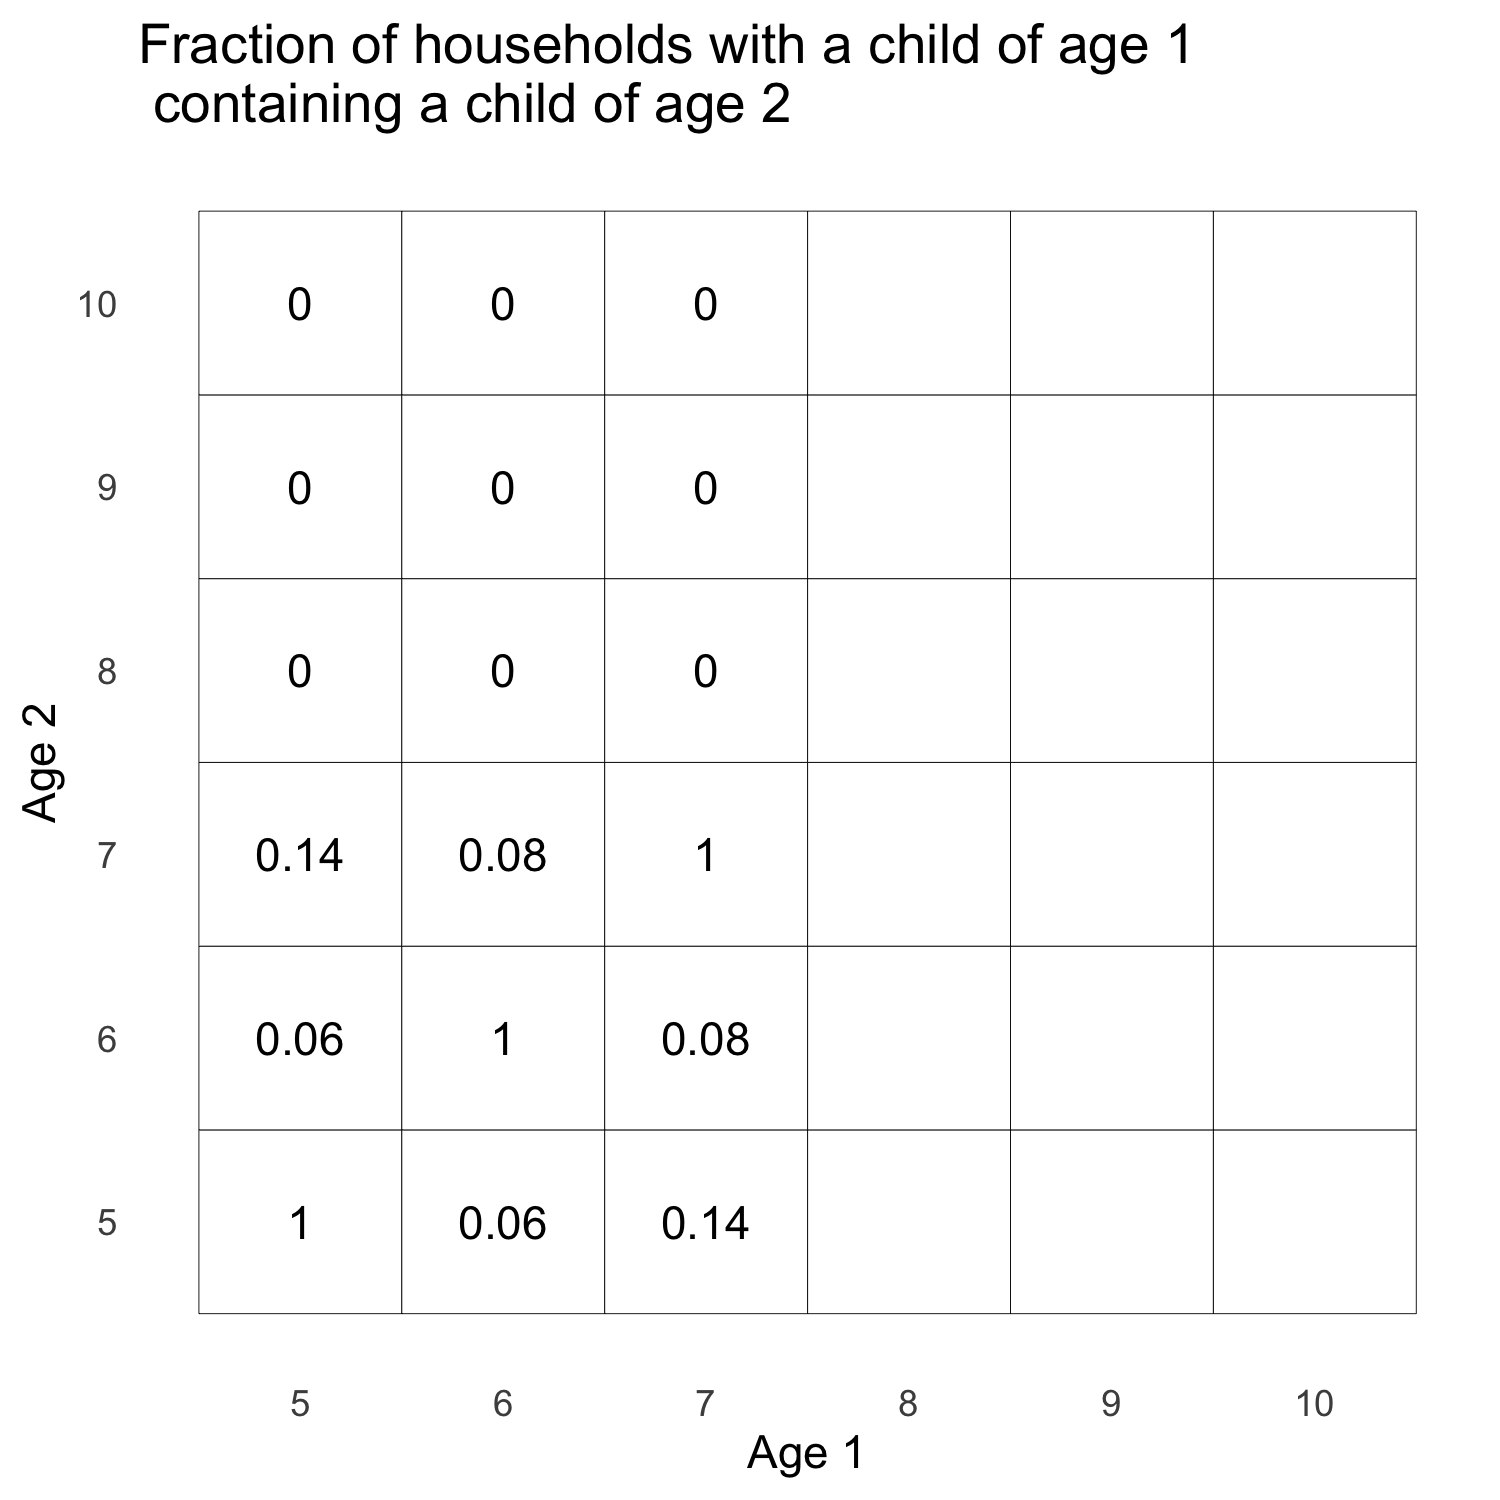
\includegraphics[width=40mm]{/Users/abilinski/Dropbox/Schools/Public code/0 - Synthetic Populations/2 - Output/sibling_heatmap_Maryland_HS.png} &
      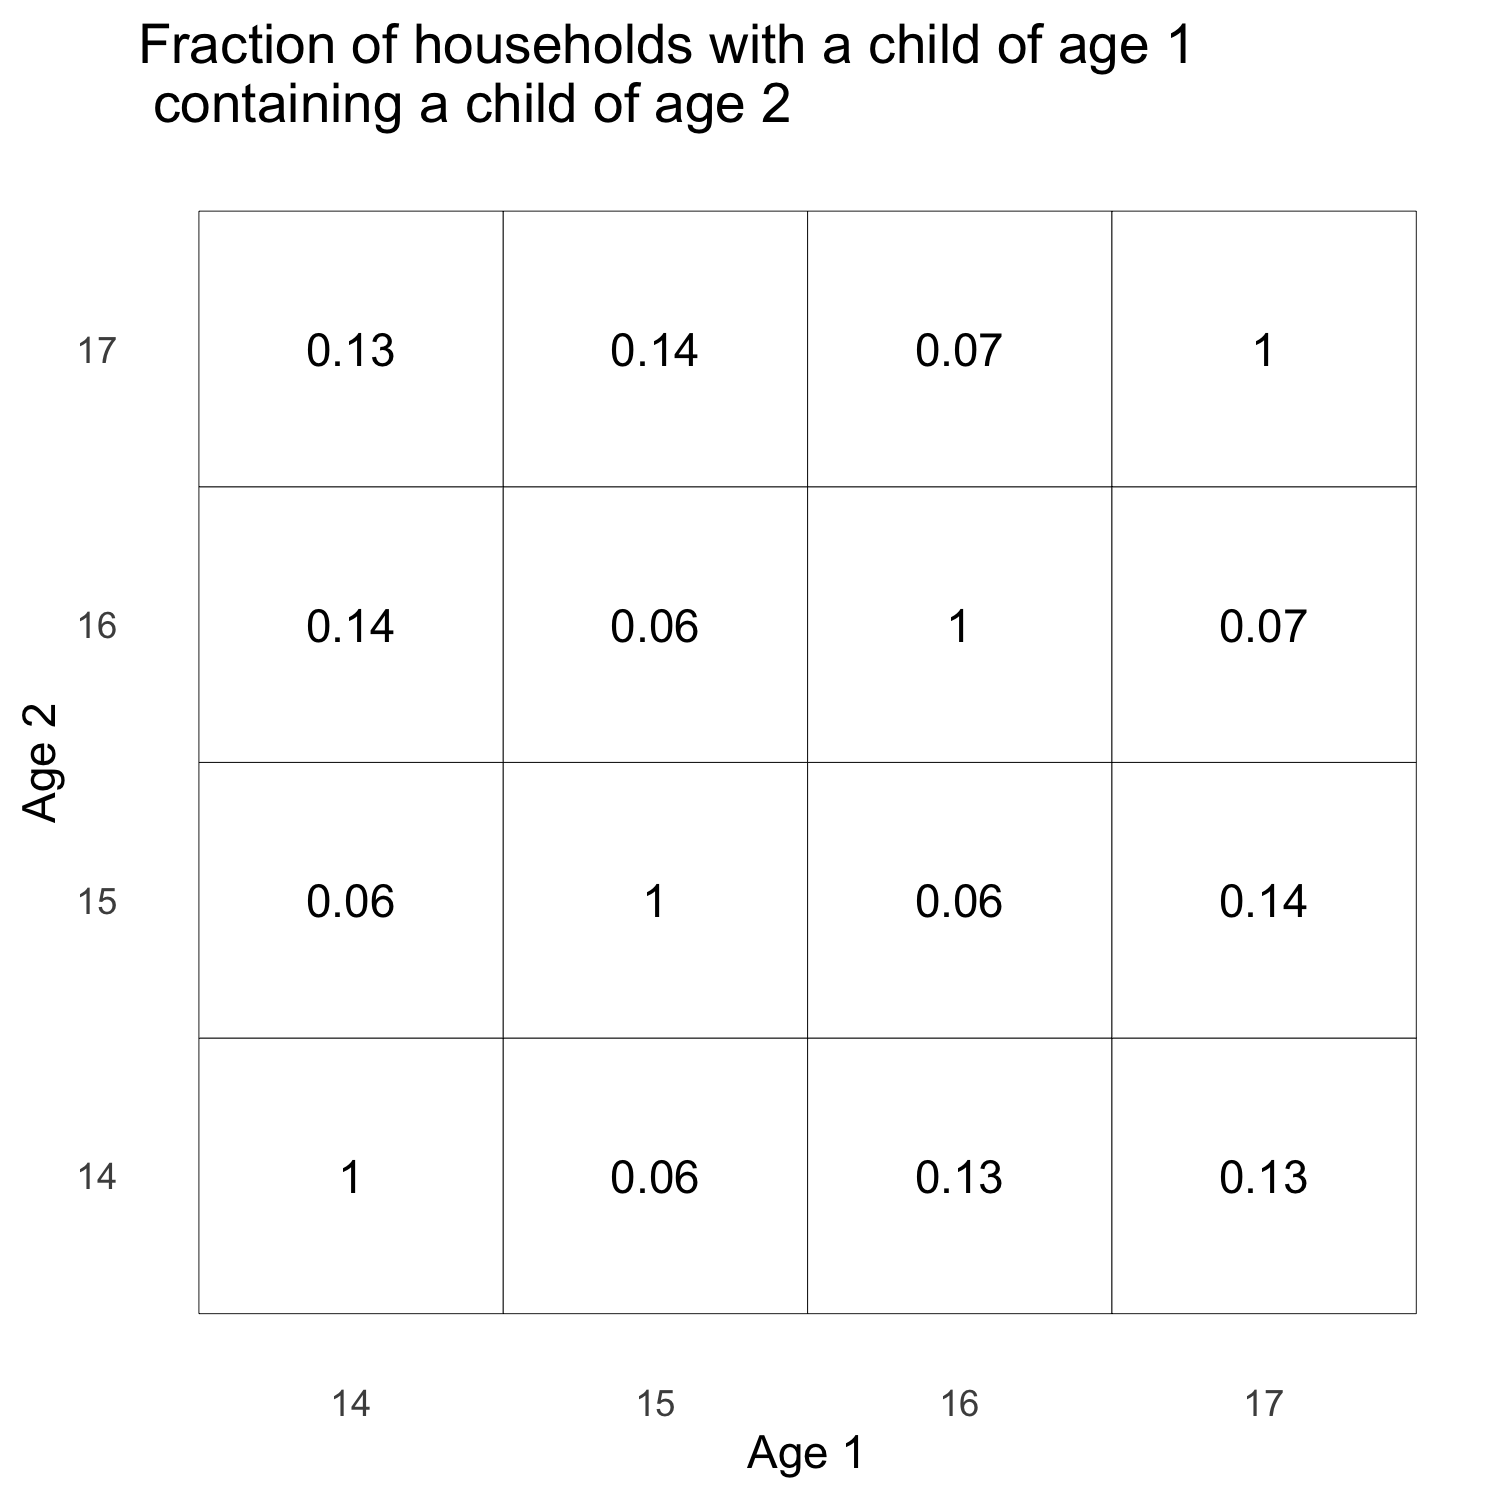
\includegraphics[width=40mm]{/Users/abilinski/Dropbox/Schools/Public code/0 - Synthetic Populations/2 - Output/sibling_heatmap_Connecticut_HS.png} &
      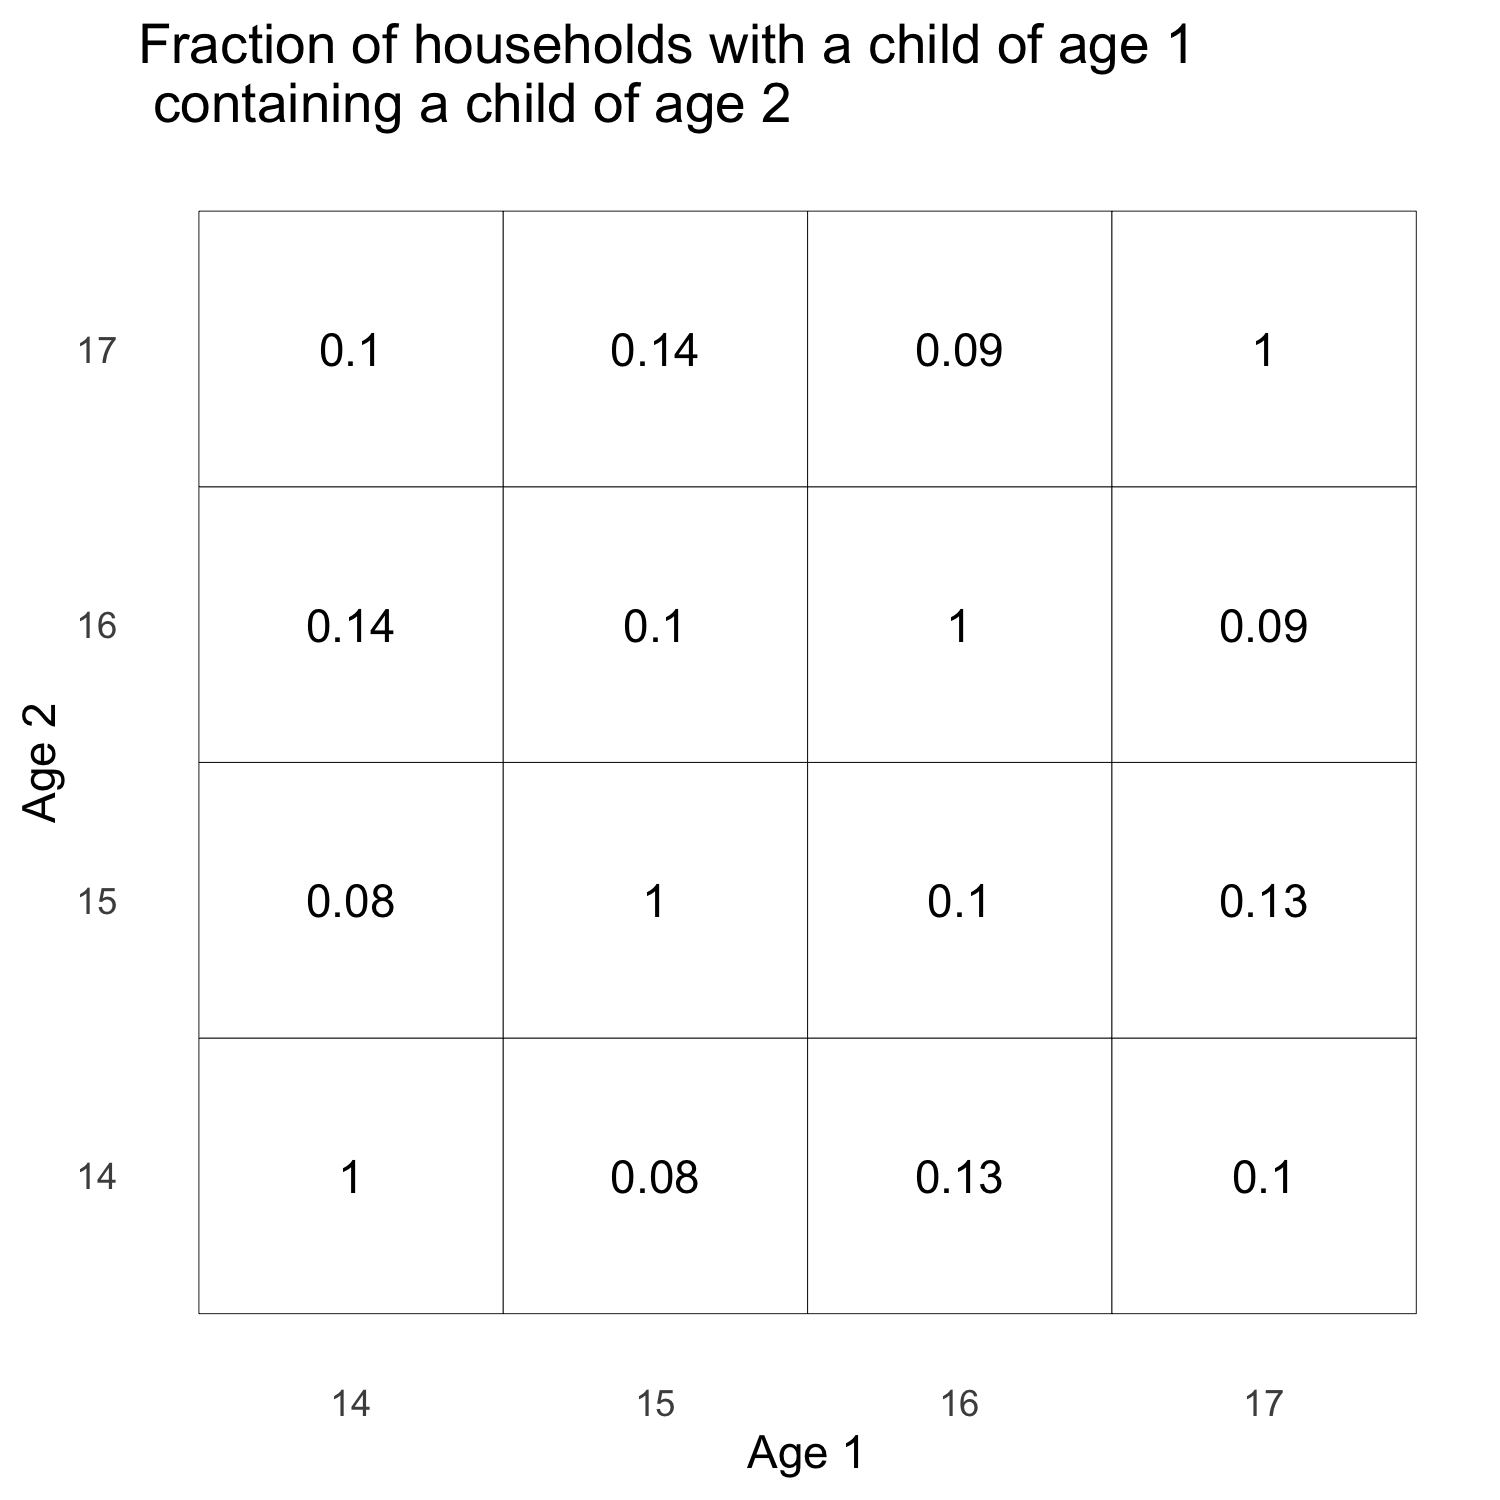
\includegraphics[width=40mm]{/Users/abilinski/Dropbox/Schools/Public code/0 - Synthetic Populations/2 - Output/sibling_heatmap_Mississippi_HS.png} &
      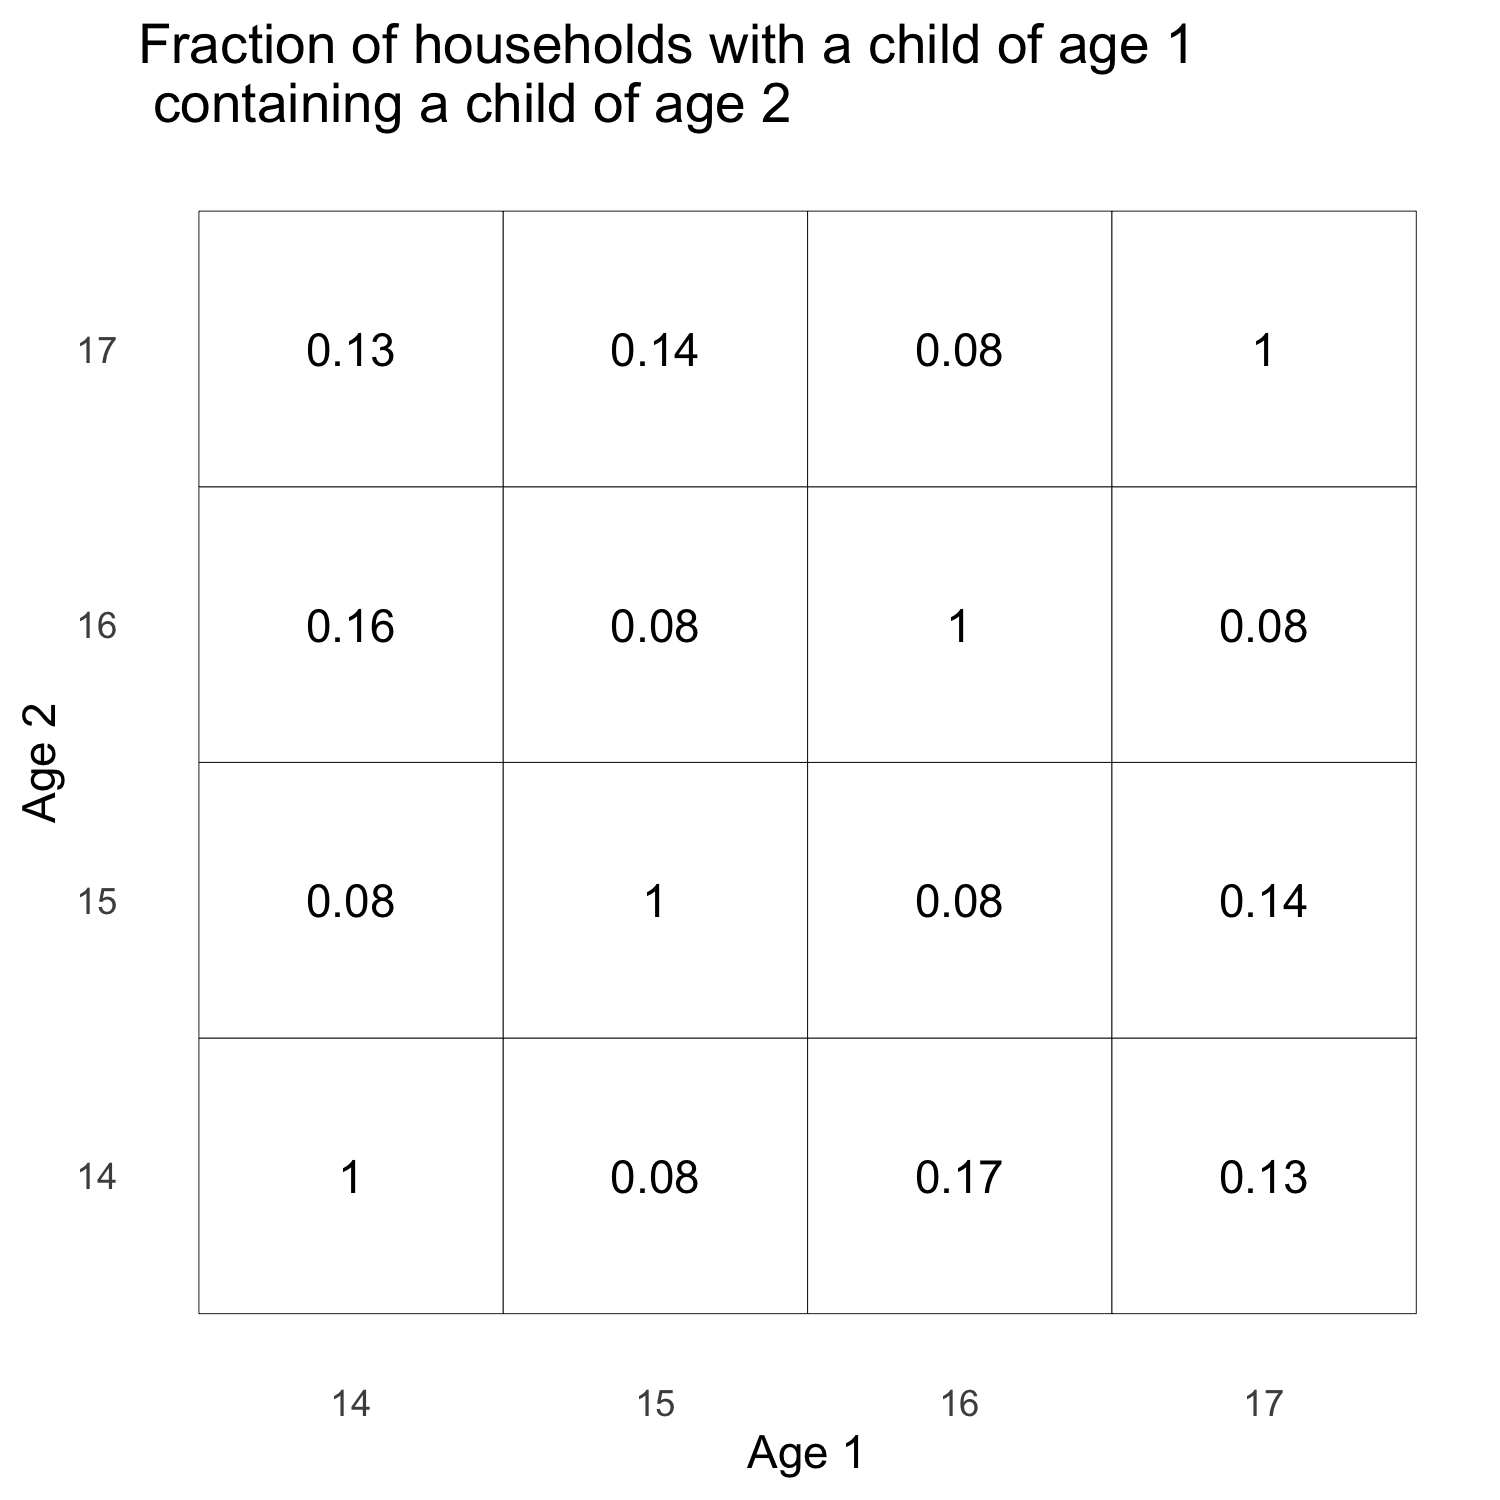
\includegraphics[width=40mm]{/Users/abilinski/Dropbox/Schools/Public code/0 - Synthetic Populations/2 - Output/sibling_heatmap_Texas_HS.png} 
    \end{tabular}

\clearpage

\hypertarget{comparison-to-observed-outbreaks}{%
\section{Comparison to observed
outbreaks}\label{comparison-to-observed-outbreaks}}

A number of factors make formal calibration challenging for this paper.
First, most data collection has been ad hoc, with some sources biased
toward reporting large outbreaks and others toward high-mitigation
schools who voluntarily collect and report data. Without comprehensive
data on school mitigation efforts, interpretation can be challenging, as
our results emphasize that a large range of outcomes is possible due to
both variation in parameters and stochastic uncertainty. Second, testing
practices vary, affecting reporting procedures. Last, the definition of
``contact'' used to construct attack rates also varies, with some
sources including even brief contacts while others require more
sustained interaction (e.g.~\textgreater15 minutes without a mask).
Overall, this section highlights why we believe our results to be
generally consistent with observed data as well as possible limitations
for future study. We emphasize that substantial uncertainty persists,
and that weekly screening or other surveillance is one of the best tools
available for understanding a specific context as well as early
detection of outbreaks.

\hypertarget{differences-in-infectiousness-and-susceptibility-by-age}{%
\subsection{Differences in infectiousness and susceptibility by
age}\label{differences-in-infectiousness-and-susceptibility-by-age}}

In our model, we assume that young children (10 and under) are both less
susceptible and less infectious than adults. To inform these
assumptions, we used a meta-analysis on child susceptibility on those
under 18-20 (\protect\hyperlink{ref-viner_susceptibility_2020}{43}),
which was consistent with best-fit model estimates
(\protect\hyperlink{ref-davies_age-dependent_2020}{67}) and another on
child infectiousness
(\protect\hyperlink{ref-zhu_meta-analysis_2020}{68}). We also used a
number of contact tracing studies suggesting not just a difference
between children and adults but also an age gradient in susceptibility
and infectiousness. These included a study from B'nei Brak, Israel on
household infections (Figure 4)
(\protect\hyperlink{ref-dattner_role_2020}{44}) and two studies from
France contrasting minimal elementary school outbreaks (despite
introductions) with a larger high school cluster in an area with early
COVID-19 exposure
(\protect\hyperlink{ref-fontanet_sars-cov-2_2020}{8},\protect\hyperlink{ref-fontanet_cluster_2020}{45}).
Limited data from Iceland, with comprehensive contact tracing and
sequencing, suggested a similar difference between young children and
adolescents in infectiousness
(\protect\hyperlink{ref-noauthor_exclusive_2020}{69}). Contact tracing
data from South Korea on infectiousness, while more difficult to
interpret due to concurrent exposures among household members and high
PPE usage of guardians of infected children
(\protect\hyperlink{ref-kim_role_2020}{70},\protect\hyperlink{ref-lee_absence_nodate}{71}),
was not inconsistent with this finding
(\protect\hyperlink{ref-park_early_nodate}{31}).

We focused on data from contact tracing studies that used comprehensive
testing of contacts because these were less likely to be biased. In
particular, we did not want to interpret evidence that children were
rarely identified as index cases
(\protect\hyperlink{ref-zhu_meta-analysis_2020}{68}) or had lower
seroprevalence in some contexts as evidence that they were less
susceptible or infectious
(\protect\hyperlink{ref-goldstein_effect_2020}{72}). These differences
could have been driven by the fact that children are less likely to have
symptoms and be tested and/or that their contacts were markedly reduced
by school closures early in the pandemic. While household contact
tracing studies with comprehensive testing avoided this issue, they
could have other biases. Children are unlikely to be caretakers of sick
individuals, and may have been shielded in houses with transmission,
particularly in the midst of an unprecedented pandemic. Nevertheless, in
general, higher household attack rates in children have been observed
for seasonal influenza and H1N1, making lower estimates for COVID-19
particularly notable
(\protect\hyperlink{ref-carcione_secondary_2011}{73}--\protect\hyperlink{ref-wu_infection_2010}{78}).

These findings nevertheless cannot differentiate between biological
explanations for lower susceptibility in younger children (e.g., lower
density of ACE2 receptor) and behavioral ones (e.g., easier to restrict
socialization). In addition, some studies suggest higher susceptibility
and/or infectiousness of young children than we include in our base case
(\protect\hyperlink{ref-bi_epidemiology_2020}{79}--\protect\hyperlink{ref-lopez_bernal_transmission_2020}{83}).
While we model these possibilities in sensitivity analyses, the bulk of
evidence on well-studied school outbreaks has pointed to important
distinctions between elementary and high school-aged children. For
example, when Israel experienced significant outbreaks upon return to
school in the early summer, there was a significant outbreak of 178
cases in a middle/high school (concentrated in grades 7-9), but
elementary school outbreaks were generally reported as smaller (e.g.~33
cases)
(\protect\hyperlink{ref-stein-zamir_large_2020}{10},\protect\hyperlink{ref-vogel_as_2020}{18}).
This difference was also apparent in informal databases, with high
schools largely responsible for outbreaks of more than 50 people
(e.g.~in New Zealand and the US prior to social distancing and
Australia, where a school outbreak was reported to be driven by high
schoolers)
(\protect\hyperlink{ref-leclerc_what_2020}{84}--\protect\hyperlink{ref-noauthor_national_nodate}{86}).
In the Netherlands, a health official was quoted saying that significant
outbreaks occurred mainly in high schools and universities prior to an
elementary school outbreak with B.1.1.7
(\protect\hyperlink{ref-vogeljan_15_school_2021}{59}). Exceptions often
included significant outbreaks among teachers (e.g., in Chile
(\protect\hyperlink{ref-torres_sars-cov-2_nodate}{12}) and Singapore
(\protect\hyperlink{ref-noauthor_covid-19_nodate-1}{87})).

\hypertarget{secondary-cases}{%
\subsection{Secondary cases}\label{secondary-cases}}

Our results are broadly consistent a few key features of observed data.
First, well-studied cases have led to no or minimal outbreaks in a
number of settings. In passive surveillance from the United Kindom
during the summer, in-school transmission was identified from 39\% of
index cases in secondary schools and 26\% of cases in primary schools
``in the context of small class or bubble sizes, half empty schools, and
extensive hygiene measures.'' This similar to what we predicted with an
A/B model in secondary schools with medium mitigation (36\%) and a low
mitigation scenario in elementary schools (23\%). No onward transmission
was found in Singapore or Ireland, each with 3 seed cases
(\protect\hyperlink{ref-yung_novel_nodate}{9},\protect\hyperlink{ref-heavey_no_2020}{88}).
In Rhode Island childcare settings, which had small class sizes, onward
transmission was documented in 4/29 index cases (14\%), consistent with
1/2 class size scenario and high mitigation (12\%)
(\protect\hyperlink{ref-link-gelles_limited_2020}{51}).

Second, several data sources showed signs of overdispersion with the
possibility of large outbreaks alongside cases without apparent
transmission. In the Rhode Island example, one outbreak involved 10
cases among contacts (10 children, four staff members, and one parent);
in another study from Australia, 9 cases in early childhood education
centers led to no onward transmission while one led to 13 infections
(\protect\hyperlink{ref-macartney_transmission_2020}{7}). If these were
indeed caused by a single index case, the level of overdispersion in our
model may not capture such extreme outcomes.

Last, teachers were often overrepresented in outbreaks even in
well-studied outbreaks, with 16\% of staff and 10\% of students having
antibodies in a Chilean outbreak across multiple school levels
(\protect\hyperlink{ref-torres_sars-cov-2_nodate}{12}). In the
Australian study, adults comprised 8/18 of secondary cases identified
(\protect\hyperlink{ref-macartney_transmission_2020}{7}).

\hypertarget{frequency-of-infections-and-subclinical-infections-in-children-compared-to-adults}{%
\subsection{Frequency of infections and subclinical infections in
children compared to
adults}\label{frequency-of-infections-and-subclinical-infections-in-children-compared-to-adults}}

Two consequential predictions from our model are that both the rate of
infections in children is lower and the rate of underdiagnosis is lower
in children. With these combined, we expect to see fewer cases in
children, but a smaller relative difference when comprehensive
surveillance and/or random testing is conducted. While some well-studied
cases in schools have led to minimal onward transmission
(\protect\hyperlink{ref-yung_novel_nodate}{9}), in several studies,
children have had higher rates of COVID-19 compared to adults such
contexts. For example, in passive surveillance from the United Kingdom,
staff had more than 4 times the COVID incidence of students per 100,000;
however in random testing, observed prevalence was equal among students
and staff \ref{@ismail_sars-cov-2_2020; @noauthor_covid-19_nodate-2}. In
elementary schools in New York in fall 2020, schools reported fewer
cases in elementary school students than in staff, but in random
surveillance testing from the same period in New York City (manually
extracted and analyzed by others), prevalence was equal in students and
staff
(\protect\hyperlink{ref-oster_opinion_2020}{89},\protect\hyperlink{ref-noauthor_covid_nodate}{90}).
While these two modes are difficult to compare directly as people who
self-isolate for symptoms are not present for random testing, the
contrast remains striking. Less systematically, a major outbreak in an
Israeli high school was detected from wide-scale testing after observing
2 unlinked community cases
(\protect\hyperlink{ref-stein-zamir_large_2020}{10}), and the first
Ontario school to participate in voluntary mass asymptomatic screening
closed after uncovering a substantial number of previously undetected
cases (\protect\hyperlink{ref-noauthor_second_2020}{91}).

\hypertarget{effective-reproduction-number}{%
\subsection{Effective reproduction
number}\label{effective-reproduction-number}}

In Figure \ref{figr}, we display the effective reproduction number
associated with different scenarios. One modeling study estimated that
from August through October 2020, there was an average effective
reproduction number of 0.54 {[}0.44-0.62{]} for children 0-9 and 0.75
{[}0.59-0.89{]} for children 10-19
(\protect\hyperlink{ref-monod_age_2020}{92}). As noted in the
introduction of this article, school openings varied considerably across
the country, but both of these fall within our range of estimates. For
elementary schools, it is consistent with full opening and high
mitigation, hybrid opening or limited attendance and medium mitigation,
or some combination of these with remote school. For high schools, it is
most consistent with high mitigation limited attendance or a hybrid
model or some combination of these with remote school.

\begin{figure}
\centering
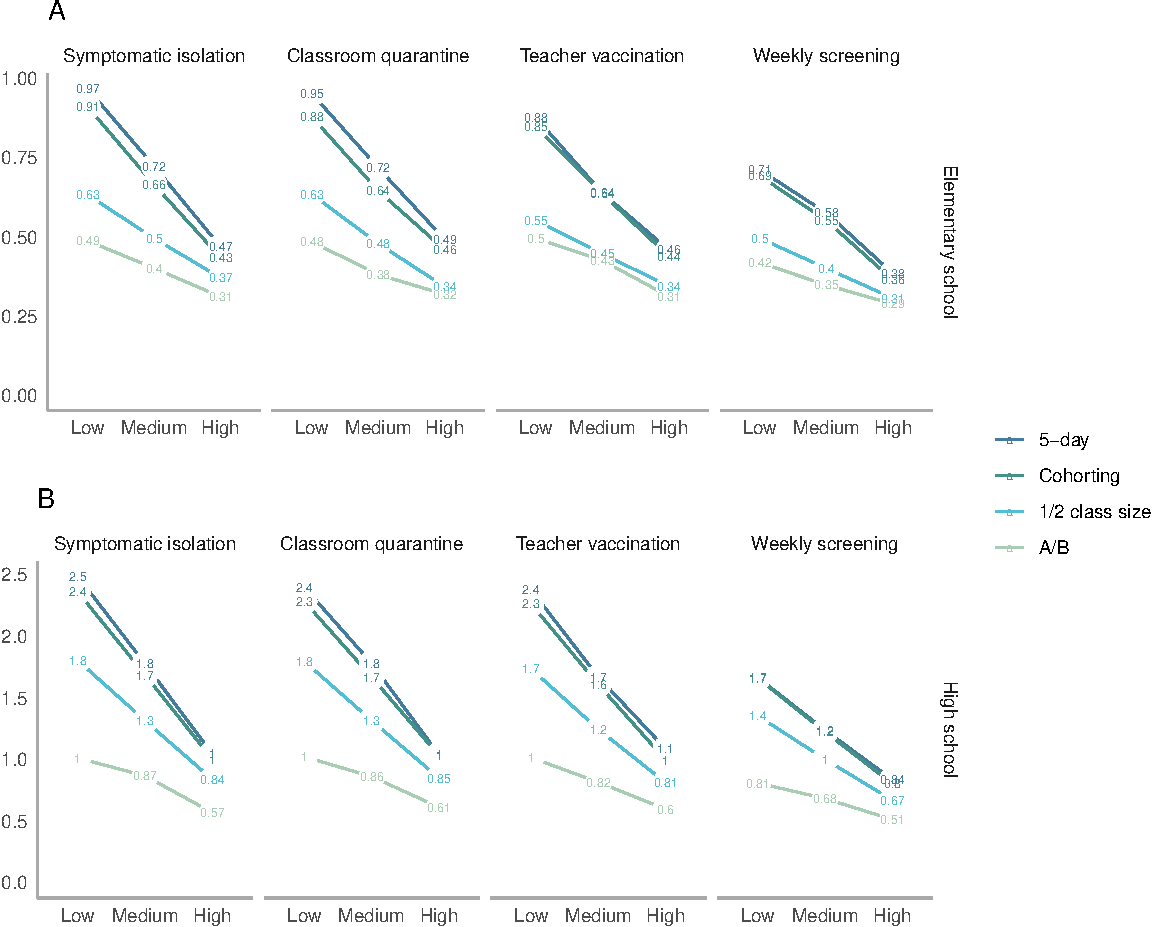
\includegraphics{Schools_draft_files/figure-latex/figr-1.pdf}
\caption{\label{figr} Effective reproduction number, defined as average
secondary transmissions following a single introduction into the school
community. The top panel shows elementary schools, where children are
assumed to be less susceptible and less infectious, while the bottom
panel shows high schools. Note that axes differ across rows. The x-axes
vary the level of prevention measure uptake, with low uptake assuming
minimal interventions and high uptake assuming intensive interventions.
Line colors correspond to scheduling strategies.}
\end{figure}

\hypertarget{population-level-studies}{%
\subsection{Population-level studies}\label{population-level-studies}}

Several population level studies have explored the relationship between
school reopening and community incidence. While we do not directly
measure community incidence, two recent studies using quasi-experimental
data to study the impact of school reopening on transmission were
consistent with our observation that there is a higher (or at least
inconclusive) risk of increased community transmission following school
reopenings when initial transmission was high
{[}(\protect\hyperlink{ref-harris_effects_nodate}{93});
goldhaber\_what\_2020{]}, contrasted to tight null effects when initial
transmission was lower.

\clearpage

\hypertarget{references}{%
\section*{References}\label{references}}
\addcontentsline{toc}{section}{References}

\hypertarget{refs}{}
\leavevmode\hypertarget{ref-noauthor_map_2020}{}%
1. Map: Coronavirus and School Closures - Education Week. Education Week
{[}Internet{]}. 2020 Mar {[}cited 2020 Jun 11{]}; Available from:
\url{https://www.edweek.org/ew/section/multimedia/map-coronavirus-and-school-closures.html}

\leavevmode\hypertarget{ref-noauthor_k-12_nodate}{}%
2. K-12 School Opening Tracker {[}Internet{]}. {[}cited 2020 Nov 25{]}.
Available from: \url{https://cai.burbio.com/school-opening-tracker/}

\leavevmode\hypertarget{ref-noauthor_more_nodate}{}%
3. More poor, Black and Hispanic students in Central Florida opt for
online learning Special Report - Orlando Sentinel {[}Internet{]}.
{[}cited 2020 Nov 25{]}. Available from:
\url{https://www.orlandosentinel.com/news/education/os-ne-race-poverty-school-online-in-person-20201105-wco4evjpxzcbjnx5sgkdsatymi-story.html}

\leavevmode\hypertarget{ref-shapiro_when_2020}{}%
4. Shapiro E. When New York City Schools Reopen, About 700,000 Students
Won't Be There. The New York Times {[}Internet{]}. 2020 Nov {[}cited
2020 Nov 25{]}; Available from:
\url{https://www.nytimes.com/2020/11/20/nyregion/nyc-schools-reopening-coronavirus.html}

\leavevmode\hypertarget{ref-shapiro_how_2020}{}%
5. Shapiro E. How de Blasio Backed Himself Into a Corner on Closing
Schools. The New York Times {[}Internet{]}. 2020 Nov {[}cited 2020 Nov
25{]}; Available from:
\url{https://www.nytimes.com/2020/11/24/nyregion/deblasio-school-reopening.html}

\leavevmode\hypertarget{ref-noauthor_combating_nodate}{}%
6. Combating COVID-19 {[}Internet{]}. President-Elect Joe Biden.
{[}cited 2020 Nov 25{]}. Available from:
\url{https://buildbackbetter.gov/priorities/covid-19/}

\leavevmode\hypertarget{ref-macartney_transmission_2020}{}%
7. Macartney K, Quinn HE, Pillsbury AJ, Koirala A, Deng L, Winkler N, et
al. Transmission of SARS-CoV-2 in Australian educational settings: A
prospective cohort study. The Lancet Child \& Adolescent Health
{[}Internet{]}. 2020 Aug {[}cited 2020 Sep 17{]};0(0). Available from:
\url{https://www.thelancet.com/journals/lanchi/article/PIIS2352-4642(20)30251-0/abstract}

\leavevmode\hypertarget{ref-fontanet_sars-cov-2_2020}{}%
8. Fontanet A, Grant R, Tondeur L, Madec Y, Grzelak L, Cailleau I, et
al. SARS-CoV-2 infection in primary schools in northern France: A
retrospective cohort study in an area of high transmission. medRxiv
{[}Internet{]}. 2020 Jun {[}cited 2020 Aug 1{]};2020.06.25.20140178.
Available from:
\url{https://www.medrxiv.org/content/10.1101/2020.06.25.20140178v2}

\leavevmode\hypertarget{ref-yung_novel_nodate}{}%
9. Yung CF, Kam K-q, Nadua KD, Chong CY, Tan NWH, Li J, et al. Novel
Coronavirus 2019 Transmission Risk in Educational Settings. Clinical
Infectious Diseases {[}Internet{]}. {[}cited 2020 Nov 25{]}; Available
from:
\url{https://academic.oup.com/cid/advance-article/doi/10.1093/cid/ciaa794/5862649}

\leavevmode\hypertarget{ref-stein-zamir_large_2020}{}%
10. Stein-Zamir C, Abramson N, Shoob H, Libal E, Bitan M, Cardash T, et
al. A large COVID-19 outbreak in a high school 10 days after schools'
reopening, Israel, May 2020. Eurosurveillance {[}Internet{]}. 2020 Jul
{[}cited 2020 Sep 17{]};25(29):2001352. Available from:
\url{https://www.eurosurveillance.org/content/10.2807/1560-7917.ES.2020.25.29.2001352}

\leavevmode\hypertarget{ref-noauthor_iowa_nodate}{}%
11. Iowa COVID-19 Tracker -- Please wear a mask. Please social distance.
{[}Internet{]}. {[}cited 2020 Nov 25{]}. Available from:
\url{https://iowacovid19tracker.org/}

\leavevmode\hypertarget{ref-torres_sars-cov-2_nodate}{}%
12. Torres JP, Piñera C, De La Maza V, Lagomarcino AJ, Simian D, Torres
B, et al. SARS-CoV-2 antibody prevalence in blood in a large school
community subject to a Covid-19 outbreak: A cross-sectional study.
Clinical Infectious Diseases {[}Internet{]}. {[}cited 2020 Sep 17{]};
Available from:
\url{https://academic.oup.com/cid/advance-article/doi/10.1093/cid/ciaa955/5869860}

\leavevmode\hypertarget{ref-auger_association_2020}{}%
13. Auger KA, Shah SS, Richardson T, Hartley D, Hall M, Warniment A, et
al. Association Between Statewide School Closure and COVID-19 Incidence
and Mortality in the US. JAMA {[}Internet{]}. 2020 Sep {[}cited 2020 Nov
25{]};324(9):859. Available from:
\url{https://jamanetwork.com/journals/jama/fullarticle/2769034}

\leavevmode\hypertarget{ref-haug_ranking_2020}{}%
14. Haug N, Geyrhofer L, Londei A, Dervic E, Desvars-Larrive A, Loreto
V, et al. Ranking the effectiveness of worldwide COVID-19 government
interventions. Nature Human Behaviour {[}Internet{]}. 2020 Nov {[}cited
2020 Nov 25{]};1--10. Available from:
\url{https://www.nature.com/articles/s41562-020-01009-0}

\leavevmode\hypertarget{ref-dong_epidemiology_2020}{}%
15. Dong Y, Mo X, Hu Y, Qi X, Jiang F, Jiang Z, et al. Epidemiology of
COVID-19 Among Children in China. Pediatrics {[}Internet{]}. 2020 Jun
{[}cited 2020 Jun 11{]};145(6). Available from:
\url{https://pediatrics.aappublications.org/content/145/6/e20200702}

\leavevmode\hypertarget{ref-noauthor_reopening_2020}{}%
16. Reopening schools in Denmark did not worsen outbreak, data shows.
Reuters {[}Internet{]}. 2020 May {[}cited 2020 Jun 11{]}; Available
from:
\url{https://www.reuters.com/article/us-health-coronavirus-denmark-reopening-idUSKBN2341N7}

\leavevmode\hypertarget{ref-pancevski_is_2020}{}%
17. Pancevski B, Dandanell N. Is It Safe to Reopen Schools? These
Countries Say Yes. Wall Street Journal {[}Internet{]}. 2020 May {[}cited
2020 Jun 11{]}; Available from:
\url{https://www.wsj.com/articles/is-it-safe-to-reopen-schools-these-countries-say-yes-11590928949}

\leavevmode\hypertarget{ref-vogel_as_2020}{}%
18. Vogel G, Couzin-FrankelNov. 18 J, 2020, Pm 5. As COVID-19 soars in
many communities, schools attempt to find ways through the crisis
{[}Internet{]}. Science AAAS. 2020 {[}cited 2020 Nov 25{]}. Available
from:
\url{https://www.sciencemag.org/news/2020/11/covid-19-soars-many-communities-schools-attempt-find-ways-through-crisis}

\leavevmode\hypertarget{ref-staton_european_2021}{}%
19. Staton B, Chazan G, Hall B, Chaffin J. European capitals follow UK
with school closures as virus surges {[}Internet{]}. 2021 {[}cited 2021
Jan 22{]}. Available from:
\url{https://www.ft.com/content/8121ca0a-4d96-4cf5-b5df-a73adc16a606}

\leavevmode\hypertarget{ref-polikoff_surveys_2020}{}%
20. Polikoff DS Anna Saavedra. Surveys show things are better for
students than they were in the spring---or do they? {[}Internet{]}.
Brookings. 2020 {[}cited 2020 Nov 20{]}. Available from:
\url{https://www.brookings.edu/blog/brown-center-chalkboard/2020/11/18/surveys-show-things-are-better-for-students-than-they-were-in-the-spring-or-do-they/}

\leavevmode\hypertarget{ref-gaudiano_missing_nodate}{}%
21. Gaudiano N. Missing: Millions of students {[}Internet{]}. POLITICO.
{[}cited 2020 Nov 25{]}. Available from: \url{https://politi.co/3dVrNxg}

\leavevmode\hypertarget{ref-leeb_mental_2020}{}%
22. Leeb RT. Mental Health--Related Emergency Department Visits Among
Children Aged 18 Years During the COVID-19 Pandemic --- United States,
January 1--October 17, 2020. MMWR Morbidity and Mortality Weekly Report
{[}Internet{]}. 2020 {[}cited 2020 Nov 30{]};69. Available from:
\url{https://www.cdc.gov/mmwr/volumes/69/wr/mm6945a3.htm}

\leavevmode\hypertarget{ref-hess_widespread_2020}{}%
23. Hess A. Widespread school closures mean 30 million kids might go
without meals {[}Internet{]}. CNBC. 2020 {[}cited 2020 Aug 1{]}.
Available from:
\url{https://www.cnbc.com/2020/03/14/widespread-school-closures-mean-30-million-kids-might-go-without-meals.html}

\leavevmode\hypertarget{ref-baron_suffering_2020}{}%
24. Baron EJ, Goldstein EG, Wallace CT. Suffering in Silence: How
COVID-19 School Closures Inhibit the Reporting of Child Maltreatment
{[}Internet{]}. Rochester, NY: Social Science Research Network; 2020 Jul
{[}cited 2020 Aug 1{]}. Report No.: ID 3601399. Available from:
\url{https://papers.ssrn.com/abstract=3664803}

\leavevmode\hypertarget{ref-bueno_bricks_2020}{}%
25. Bueno C. Bricks and Mortar vs. Computers and Modems: The Impacts of
Enrollment in K-12 Virtual Schools {[}Internet{]}. Rochester, NY: Social
Science Research Network; 2020 Jul {[}cited 2020 Aug 1{]}. Report No.:
ID 3642969. Available from:
\url{https://papers.ssrn.com/abstract=3642969}

\leavevmode\hypertarget{ref-lempel_costs_2009}{}%
26. Lempel H, Hammond R, Epstein J. Costs of School Closure
{[}Internet{]}. Brookings Institute; 2009 Sep {[}cited 2020 Aug 1{]}.
Available from:
\url{https://www.brookings.edu/wp-content/uploads/2016/06/0930_school_closure_presentation.pdf}

\leavevmode\hypertarget{ref-soland_impact_2020}{}%
27. Soland J, Kuhfeld M, Tarasawa B, Johnson A, Ruzek E, Liu J. The
impact of COVID-19 on student achievement and what it may mean for
educators {[}Internet{]}. Brookings. 2020 {[}cited 2020 Aug 1{]}.
Available from:
\url{https://www.brookings.edu/blog/brown-center-chalkboard/2020/05/27/the-impact-of-covid-19-on-student-achievement-and-what-it-may-mean-for-educators/}

\leavevmode\hypertarget{ref-cohen_schools_2020}{}%
28. Cohen JA, Mistry D, Kerr CC, Klein DJ. Schools are not islands:
Balancing COVID-19 risk and educational benefits using structural and
temporal countermeasures {[}Internet{]}. Epidemiology; 2020 Sep {[}cited
2020 Sep 17{]}. Available from:
\url{http://medrxiv.org/lookup/doi/10.1101/2020.09.08.20190942}

\leavevmode\hypertarget{ref-espana_impacts_2020}{}%
29. Espana G, Cavany S, Oidtman RJ, Barbera C, Costello A, Lerch A, et
al. Impacts of K-12 school reopening on the COVID-19 epidemic in
Indiana, USA. medRxiv {[}Internet{]}. 2020 Sep {[}cited 2020 Sep
17{]};2020.08.22.20179960. Available from:
\url{https://www.medrxiv.org/content/10.1101/2020.08.22.20179960v2}

\leavevmode\hypertarget{ref-head_effect_2020}{}%
30. Head JR, Andrejko K, Cheng Q, Collender PA, Phillips S, Boser A, et
al. The effect of school closures and reopening strategies on COVID-19
infection dynamics in the San Francisco Bay Area: A cross-sectional
survey and modeling analysis. medRxiv {[}Internet{]}. 2020 Aug {[}cited
2020 Sep 17{]};2020.08.06.20169797. Available from:
\url{https://www.medrxiv.org/content/10.1101/2020.08.06.20169797v1}

\leavevmode\hypertarget{ref-park_early_nodate}{}%
31. Park YJ, Choe YJ, Park O, Park SY, Kim Y-M, Kim J, et al. Early
Release - Contact Tracing during Coronavirus Disease Outbreak, South
Korea, 2020 - Volume 26, Number 10---October 2020 - Emerging Infectious
Diseases journal - CDC. {[}cited 2020 Aug 1{]}; Available from:
\url{https://wwwnc.cdc.gov/eid/article/26/10/20-1315_article}

\leavevmode\hypertarget{ref-cdc_covid-19_2020}{}%
32. CDC. COVID-19 and Your Health {[}Internet{]}. Centers for Disease
Control and Prevention. 2020 {[}cited 2021 Jan 4{]}. Available from:
\url{https://www.cdc.gov/coronavirus/2019-ncov/if-you-are-sick/quarantine.html}

\leavevmode\hypertarget{ref-gallup_inc_willingness_2020}{}%
33. Gallup I. Willingness to Get COVID-19 Vaccine Ticks Up to 63\% in
U.S. {[}Internet{]}. Gallup.com. 2020 {[}cited 2021 Jan 4{]}. Available
from:
\url{https://news.gallup.com/poll/327425/willingness-covid-vaccine-ticks.aspx}

\leavevmode\hypertarget{ref-will_school_2020}{}%
34. Will M. School Workers May Get Early Shot at COVID-19 Vaccine. Will
They Take It? {[}Internet{]}. Education Week. 2020 {[}cited 2021 Jan
4{]}. Available from:
\url{https://www.edweek.org/leadership/school-workers-may-get-early-shot-at-covid-19-vaccine-will-they-take-it/2020/12}

\leavevmode\hypertarget{ref-polack_safety_2020}{}%
35. Polack FP, Thomas SJ, Kitchin N, Absalon J, Gurtman A, Lockhart S,
et al. Safety and Efficacy of the BNT162b2 mRNA Covid-19 Vaccine. New
England Journal of Medicine {[}Internet{]}. 2020 Dec {[}cited 2021 Jan
4{]};383(27):2603--15. Available from:
\url{https://doi.org/10.1056/NEJMoa2034577}

\leavevmode\hypertarget{ref-wheaton_us_2014}{}%
36. Wheaton WD. U.S. Synthetic Population 2010 Version 1.0 Quick Start
Guide, RTI International. 2014 May.

\leavevmode\hypertarget{ref-noauthor_digest_nodate}{}%
37. Digest of Education Statistics, 2019 {[}Internet{]}. {[}cited 2020
Dec 12{]}. Available from:
\url{https://nces.ed.gov/programs/digest/d19/tables/dt19_216.40.asp?current=yes}

\leavevmode\hypertarget{ref-madewell_household_2020}{}%
38. Madewell ZJ, Yang Y, Longini IM, Halloran ME, Dean NE. Household
Transmission of SARS-CoV-2: A Systematic Review and Meta-analysis. JAMA
Network Open {[}Internet{]}. 2020 Dec {[}cited 2021 Jan
3{]};3(12):e2031756. Available from:
\url{https://jamanetwork.com/journals/jamanetworkopen/fullarticle/2774102}

\leavevmode\hypertarget{ref-fung_household_2020}{}%
39. Fung HF, Martinez L, Alarid-Escudero F, Salomon JA, Studdert DM,
Andrews JR, et al. The Household Secondary Attack Rate of Severe Acute
Respiratory Syndrome Coronavirus 2 (SARS-CoV-2): A Rapid Review.
Clinical Infectious Diseases {[}Internet{]}. 2020 Oct {[}cited 2021 Jan
3{]};ciaa1558. Available from:
\url{https://academic.oup.com/cid/advance-article/doi/10.1093/cid/ciaa1558/5921151}

\leavevmode\hypertarget{ref-cheng_contact_2020}{}%
40. Cheng H-Y, Jian S-W, Liu D-P, Ng T-C, Huang W-T, Lin H-H. Contact
Tracing Assessment of COVID-19 Transmission Dynamics in Taiwan and Risk
at Different Exposure Periods Before and After Symptom Onset. JAMA
Internal Medicine {[}Internet{]}. 2020 May {[}cited 2020 Jun 2{]};
Available from:
\url{https://jamanetwork.com/journals/jamainternalmedicine/fullarticle/2765641}

\leavevmode\hypertarget{ref-clapp_evaluation_2020}{}%
41. Clapp PW, Sickbert-Bennett EE, Samet JM, Berntsen J, Zeman KL,
Anderson DJ, et al. Evaluation of Cloth Masks and Modified Procedure
Masks as Personal Protective Equipment for the Public During the
COVID-19 Pandemic. JAMA Internal Medicine {[}Internet{]}. 2020 Dec
{[}cited 2021 Jan 4{]}; Available from:
\url{https://jamanetwork.com/journals/jamainternalmedicine/fullarticle/2774266}

\leavevmode\hypertarget{ref-chu_physical_2020}{}%
42. Chu DK, Akl EA, Duda S, Solo K, Yaacoub S, Schünemann HJ, et al.
Physical distancing, face masks, and eye protection to prevent
person-to-person transmission of SARS-CoV-2 and COVID-19: A systematic
review and meta-analysis. The Lancet {[}Internet{]}. 2020 Jun {[}cited
2021 Jan 4{]};395(10242):1973--87. Available from:
\url{https://linkinghub.elsevier.com/retrieve/pii/S0140673620311429}

\leavevmode\hypertarget{ref-viner_susceptibility_2020}{}%
43. Viner RM, Mytton OT, Bonell C, Melendez-Torres GJ, Ward J, Hudson L,
et al. Susceptibility to SARS-CoV-2 Infection Among Children and
Adolescents Compared With Adults: A Systematic Review and Meta-analysis.
JAMA Pediatrics {[}Internet{]}. 2020 Sep {[}cited 2021 Jan 6{]};
Available from:
\url{https://jamanetwork.com/journals/jamapediatrics/fullarticle/2771181}

\leavevmode\hypertarget{ref-dattner_role_2020}{}%
44. Dattner I, Goldberg Y, Katriel G, Yaari R, Gal N, Miron Y, et al.
The role of children in the spread of COVID-19: Using household data
from Bnei Brak, Israel, to estimate the relative susceptibility and
infectivity of children {[}Internet{]}. Infectious Diseases (except
HIV/AIDS); 2020 Jun {[}cited 2020 Jun 19{]}. Available from:
\url{http://medrxiv.org/lookup/doi/10.1101/2020.06.03.20121145}

\leavevmode\hypertarget{ref-fontanet_cluster_2020}{}%
45. Fontanet A, Tondeur L, Madec Y, Grant R, Besombes C, Jolly N, et al.
Cluster of COVID-19 in northern France: A retrospective closed cohort
study. medRxiv {[}Internet{]}. 2020 Apr {[}cited 2020 Jul
9{]};2020.04.18.20071134. Available from:
\url{https://www.medrxiv.org/content/10.1101/2020.04.18.20071134v1}

\leavevmode\hypertarget{ref-byambasuren_estimating_2020}{}%
46. Byambasuren O, Cardona M, Bell K, Clark J, McLaws M-L, Glasziou P.
Estimating the extent of asymptomatic COVID-19 and its potential for
community transmission: Systematic review and meta-analysis. Official
Journal of the Association of Medical Microbiology and Infectious
Disease Canada {[}Internet{]}. 2020 Dec {[}cited 2021 Jan
4{]};5(4):223--34. Available from:
\url{https://jammi.utpjournals.press/doi/10.3138/jammi-2020-0030}

\leavevmode\hypertarget{ref-kerr_covasim_2020}{}%
47. Kerr CC, Stuart RM, Mistry D, Abeysuriya RG, Hart G, Rosenfeld K, et
al. Covasim: An agent-based model of COVID-19 dynamics and
interventions. medRxiv {[}Internet{]}. 2020 May {[}cited 2020 Jun
2{]};2020.05.10.20097469. Available from:
\url{https://www.medrxiv.org/content/10.1101/2020.05.10.20097469v1}

\leavevmode\hypertarget{ref-endo_estimating_2020}{}%
48. Endo A, Centre for the Mathematical Modelling of Infectious Diseases
COVID-19 Working Group, Abbott S, Kucharski AJ, Funk S. Estimating the
overdispersion in COVID-19 transmission using outbreak sizes outside
China. Wellcome Open Research {[}Internet{]}. 2020 Apr {[}cited 2020 Jun
11{]};5:67. Available from:
\url{https://wellcomeopenresearch.org/articles/5-67/v1}

\leavevmode\hypertarget{ref-noauthor_schools_nodate}{}%
49. Schools and the Path to Zero -- Pandemics Explained {[}Internet{]}.
{[}cited 2021 Jan 20{]}. Available from:
\url{https://globalepidemics.org/2020/12/18/schools-and-the-path-to-zero/}

\leavevmode\hypertarget{ref-cdc_communities_2020}{}%
50. CDC. Communities, Schools, Workplaces, \& Events {[}Internet{]}.
Centers for Disease Control and Prevention. 2020 {[}cited 2020 Nov
25{]}. Available from:
\url{https://www.cdc.gov/coronavirus/2019-ncov/community/schools-childcare/indicators.html}

\leavevmode\hypertarget{ref-link-gelles_limited_2020}{}%
51. Link-Gelles R. Limited Secondary Transmission of SARS-CoV-2 in Child
Care Programs --- Rhode Island, June 1--July 31, 2020. MMWR Morbidity
and Mortality Weekly Report {[}Internet{]}. 2020 {[}cited 2020 Sep
17{]};69. Available from:
\url{https://www.cdc.gov/mmwr/volumes/69/wr/mm6934e2.htm}

\leavevmode\hypertarget{ref-ladhani_prospective_nodate}{}%
52. Ladhani S, Ahmad S, Garstang J, Brent AJ, Brent B. Prospective
active national surveillance of preschools and primary schools for
SARS-CoV-2 infection and transmission in England, June 2020.:23.

\leavevmode\hypertarget{ref-noauthor_bwh_nodate}{}%
53. BWH Press Release - Brigham and Women's Hospital {[}Internet{]}.
{[}cited 2020 Nov 25{]}. Available from:
\url{https://www.brighamandwomens.org/about-bwh/newsroom/press-releases-detail?id=3684}

\leavevmode\hypertarget{ref-althouse_stochasticity_nodate}{}%
54. Althouse BM, Wenger EA, Miller JC, Allard A. Stochasticity and
heterogeneity in the transmission dynamics of SARS-CoV-2.:10.

\leavevmode\hypertarget{ref-sun_impact_2020}{}%
55. Sun K, Viboud C. Impact of contact tracing on SARS-CoV-2
transmission. The Lancet Infectious Diseases {[}Internet{]}. 2020 Apr
{[}cited 2020 May 14{]};0(0). Available from:
\url{https://www.thelancet.com/journals/laninf/article/PIIS1473-3099(20)30357-1/abstract}

\leavevmode\hypertarget{ref-tupper_event-specific_2020}{}%
56. Tupper P, Boury H, Yerlanov M, Colijn C. Event-specific
interventions to minimize COVID-19 transmission. Proceedings of the
National Academy of Sciences {[}Internet{]}. 2020 Nov {[}cited 2020 Nov
25{]}; Available from:
\url{https://www.pnas.org/content/early/2020/11/18/2019324117}

\leavevmode\hypertarget{ref-meyerowitz_transmission_2020}{}%
57. Meyerowitz EA, Richterman A, Gandhi RT, Sax PE. Transmission of
SARS-CoV-2: A Review of Viral, Host, and Environmental Factors. Annals
of Internal Medicine {[}Internet{]}. 2020 Sep {[}cited 2020 Nov 25{]};
Available from:
\url{https://www.acpjournals.org/doi/full/10.7326/M20-5008}

\leavevmode\hypertarget{ref-volz_transmission_2021}{}%
58. Volz E, Mishra S, Chand M, Barrett JC, Johnson R, Geidelberg L, et
al. Transmission of SARS-CoV-2 Lineage B.1.1.7 in England: Insights from
linking epidemiological and genetic data. medRxiv {[}Internet{]}. 2021
Jan {[}cited 2021 Jan 6{]};2020.12.30.20249034. Available from:
\url{https://www.medrxiv.org/content/10.1101/2020.12.30.20249034v2}

\leavevmode\hypertarget{ref-vogeljan_15_school_2021}{}%
59. VogelJan. 15 G, 2021, Pm 4. School risk calculations scrambled by
fast-spreading virus strains {[}Internet{]}. Science AAAS. 2021 {[}cited
2021 Jan 22{]}. Available from:
\url{https://www.sciencemag.org/news/2021/01/new-coronavirus-variant-scrambles-school-risk-calculations}

\leavevmode\hypertarget{ref-han_clinical_2020}{}%
60. Han MS, Choi EH, Chang SH, Jin B-L, Lee EJ, Kim BN, et al. Clinical
Characteristics and Viral RNA Detection in Children With Coronavirus
Disease 2019 in the Republic of Korea. JAMA Pediatrics {[}Internet{]}.
2020 Aug {[}cited 2020 Dec 13{]}; Available from:
\url{https://doi.org/10.1001/jamapediatrics.2020.3988}

\leavevmode\hypertarget{ref-lauer_incubation_2020}{}%
61. Lauer SA, Grantz KH, Bi Q, Jones FK, Zheng Q, Meredith HR, et al.
The Incubation Period of Coronavirus Disease 2019 (COVID-19) From
Publicly Reported Confirmed Cases: Estimation and Application. Annals of
Internal Medicine {[}Internet{]}. 2020 Mar {[}cited 2020 Jun
2{]};172(9):577--82. Available from:
\url{https://www.acpjournals.org/doi/10.7326/M20-0504}

\leavevmode\hypertarget{ref-li_early_2020}{}%
62. Li Q, Guan X, Wu P, Wang X, Zhou L, Tong Y, et al. Early
Transmission Dynamics in Wuhan, China, of Novel Coronavirus--Infected
Pneumonia. New England Journal of Medicine {[}Internet{]}. 2020 Jan
{[}cited 2020 Mar 14{]};0(0):null. Available from:
\url{https://doi.org/10.1056/NEJMoa2001316}

\leavevmode\hypertarget{ref-gatto_spread_2020}{}%
63. Gatto M, Bertuzzo E, Mari L, Miccoli S, Carraro L, Casagrandi R, et
al. Spread and dynamics of the COVID-19 epidemic in Italy: Effects of
emergency containment measures. Proceedings of the National Academy of
Sciences {[}Internet{]}. 2020 May {[}cited 2020 Jun
2{]};117(19):10484--91. Available from:
\url{http://www.pnas.org/lookup/doi/10.1073/pnas.2004978117}

\leavevmode\hypertarget{ref-he_temporal_2020}{}%
64. He X, Lau EHY, Wu P, Deng X, Wang J, Hao X, et al. Temporal dynamics
in viral shedding and transmissibility of COVID-19. Nature Medicine
{[}Internet{]}. 2020 Apr {[}cited 2020 Apr 29{]};1--4. Available from:
\url{https://www.nature.com/articles/s41591-020-0869-5}

\leavevmode\hypertarget{ref-he_relative_2020}{}%
65. He D, Zhao S, Lin Q, Zhuang Z, Cao P, Wang MH, et al. The relative
transmissibility of asymptomatic COVID-19 infections among close
contacts. International Journal of Infectious Diseases {[}Internet{]}.
2020 May {[}cited 2020 Jun 2{]};94:145--7. Available from:
\url{http://www.sciencedirect.com/science/article/pii/S1201971220302502}

\leavevmode\hypertarget{ref-firth_combining_2020}{}%
66. Firth JA, Hellewell J, Klepac P, Kissler SM, CMMID COVID-19 working
group, Kucharski AJ, et al. Combining fine-scale social contact data
with epidemic modelling reveals interactions between contact tracing,
quarantine, testing and physical distancing for controlling COVID-19
{[}Internet{]}. Epidemiology; 2020 May {[}cited 2020 Jun 2{]}. Available
from: \url{http://medrxiv.org/lookup/doi/10.1101/2020.05.26.20113720}

\leavevmode\hypertarget{ref-davies_age-dependent_2020}{}%
67. Davies NG, Klepac P, Liu Y, Prem K, Jit M, Eggo RM. Age-dependent
effects in the transmission and control of COVID-19 epidemics. Nature
Medicine {[}Internet{]}. 2020 Aug {[}cited 2021 Jan
24{]};26(8):1205--11. Available from:
\url{https://www.nature.com/articles/s41591-020-0962-9}

\leavevmode\hypertarget{ref-zhu_meta-analysis_2020}{}%
68. Zhu Y, Bloxham CJ, Hulme KD, Sinclair JE, Tong ZWM, Steele LE, et
al. A meta-analysis on the role of children in SARS-CoV-2 in household
transmission clusters. medRxiv {[}Internet{]}. 2020 Dec {[}cited 2021
Jan 24{]};2020.03.26.20044826. Available from:
\url{https://www.medrxiv.org/content/10.1101/2020.03.26.20044826v2}

\leavevmode\hypertarget{ref-noauthor_exclusive_2020}{}%
69. Exclusive: Kids catch and spread coronavirus half as much as adults,
Iceland study confirms {[}Internet{]}. Science. 2020 {[}cited 2021 Jan
24{]}. Available from:
\url{https://www.nationalgeographic.com/science/2020/12/we-now-know-how-much-children-spread-coronavirus/}

\leavevmode\hypertarget{ref-kim_role_2020}{}%
70. Kim J, Choe YJ, Lee J, Park YJ, Park O, Han MS, et al. Role of
children in household transmission of COVID-19. Archives of Disease in
Childhood {[}Internet{]}. 2020 Aug {[}cited 2021 Jan 24{]}; Available
from:
\url{https://adc.bmj.com/content/early/2020/08/06/archdischild-2020-319910}

\leavevmode\hypertarget{ref-lee_absence_nodate}{}%
71. Lee EJ, Kim DH, Chang SH, Suh SB, Lee J, Lee H, et al. Absence of
SARS-CoV-2 Transmission from Children in Isolation to Guardians, South
Korea - Volume 27, Number 1---January 2021 - Emerging Infectious
Diseases journal - CDC. {[}cited 2021 Jan 24{]}; Available from:
\url{https://wwwnc.cdc.gov/eid/article/27/1/20-3450_article}

\leavevmode\hypertarget{ref-goldstein_effect_2020}{}%
72. Goldstein E, Lipsitch M, Cevik M. On the Effect of Age on the
Transmission of SARS-CoV-2 in Households, Schools, and the Community.
The Journal of Infectious Diseases {[}Internet{]}. 2020 Oct {[}cited
2021 Jan 24{]};(jiaa691). Available from:
\url{https://doi.org/10.1093/infdis/jiaa691}

\leavevmode\hypertarget{ref-carcione_secondary_2011}{}%
73. Carcione D, Giele CM, Goggin LS, Kwan KS, Smith DW, Dowse GK, et al.
Secondary attack rate of pandemic influenza A(H1N1)2009 in Western
Australian households, 29 May--7 August 2009. Eurosurveillance
{[}Internet{]}. 2011 Jan {[}cited 2020 Jun 19{]};16(3):19765. Available
from:
\url{https://www.eurosurveillance.org/content/10.2807/ese.16.03.19765-en}

\leavevmode\hypertarget{ref-odaira_assessment_2009}{}%
74. Odaira F, Takahashi H, Toyokawa T, Tsuchihashi Y, Kodama T, Yahata
Y, et al. Assessment of secondary attack rate and effectiveness of
antiviral prophylaxis among household contacts in an influenza A(H1N1)v
outbreak in Kobe, Japan, May--June 2009. Eurosurveillance
{[}Internet{]}. 2009 Sep {[}cited 2020 Jun 19{]};14(35):19320. Available
from:
\url{https://www.eurosurveillance.org/content/10.2807/ese.14.35.19320-en}

\leavevmode\hypertarget{ref-sikora_transmission_2010}{}%
75. Sikora C, Fan S, Golonka R, Sturtevant D, Gratrix J, Lee BE, et al.
Transmission of pandemic influenza A (H1N1) 2009 within households:
Edmonton, Canada. Journal of Clinical Virology {[}Internet{]}. 2010 Oct
{[}cited 2020 Jun 19{]};49(2):90--3. Available from:
\url{http://www.sciencedirect.com/science/article/pii/S1386653210002593}

\leavevmode\hypertarget{ref-sugimoto_effect_2011}{}%
76. Sugimoto JD, Borse NN, Ta ML, Stockman LJ, Fischer GE, Yang Y, et
al. The Effect of Age on Transmission of 2009 Pandemic Influenza A
(H1N1) in a Camp and Associated Households. Epidemiology (Cambridge,
Mass) {[}Internet{]}. 2011 Mar {[}cited 2020 Jun 19{]};22(2). Available
from: \url{https://www.ncbi.nlm.nih.gov/pmc/articles/PMC3755879/}

\leavevmode\hypertarget{ref-klick_transmissibility_2011}{}%
77. Klick B, Nishiura H, Ng S, Fang VJ, Leung GM, Malik Peiris JS, et
al. Transmissibility of seasonal and pandemic influenza in a cohort of
households in Hong Kong in 2009. Epidemiology (Cambridge, Mass)
{[}Internet{]}. 2011 Nov {[}cited 2020 Jun 19{]};22(6):793--6. Available
from: \url{https://www.ncbi.nlm.nih.gov/pmc/articles/PMC3206962/}

\leavevmode\hypertarget{ref-wu_infection_2010}{}%
78. Wu JT, Ma ESK, Lee CK, Chu DKW, Ho P-L, Shen AL, et al. The
Infection Attack Rate and Severity of 2009 Pandemic H1N1 Influenza in
Hong Kong. Clinical Infectious Diseases {[}Internet{]}. 2010 Nov
{[}cited 2020 Jun 19{]};51(10):1184--91. Available from:
\url{https://academic.oup.com/cid/article/51/10/1184/393386}

\leavevmode\hypertarget{ref-bi_epidemiology_2020}{}%
79. Bi Q, Wu Y, Mei S, Ye C, Zou X, Zhang Z, et al. Epidemiology and
transmission of COVID-19 in 391 cases and 1286 of their close contacts
in Shenzhen, China: A retrospective cohort study. The Lancet Infectious
Diseases {[}Internet{]}. 2020 Aug {[}cited 2021 Jan 24{]};20(8):911--9.
Available from:
\url{https://www.thelancet.com/journals/laninf/article/PIIS1473-3099(20)30287-5/abstract}

\leavevmode\hypertarget{ref-fateh-moghadam_contact_2020}{}%
80. Fateh-Moghadam P, Battisti L, Molinaro S, Fontanari S, Dallago G,
Binkin N, et al. Contact tracing during Phase I of the COVID-19 pandemic
in the Province of Trento, Italy: Key findings and recommendations.
medRxiv {[}Internet{]}. 2020 Jul {[}cited 2021 Jan
24{]};2020.07.16.20127357. Available from:
\url{https://www.medrxiv.org/content/10.1101/2020.07.16.20127357v1}

\leavevmode\hypertarget{ref-li_household_2021}{}%
81. Li F, Li Y-Y, Liu M-J, Fang L-Q, Dean NE, Wong GWK, et al. Household
transmission of SARS-CoV-2 and risk factors for susceptibility and
infectivity in Wuhan: A retrospective observational study. The Lancet
Infectious Diseases {[}Internet{]}. 2021 Jan {[}cited 2021 Jan
24{]};0(0). Available from:
\url{https://www.thelancet.com/journals/laninf/article/PIIS1473-3099(20)30981-6/abstract}

\leavevmode\hypertarget{ref-grijalva_transmission_2020}{}%
82. Grijalva CG. Transmission of SARS-COV-2 Infections in Households ---
Tennessee and Wisconsin, April--September 2020. MMWR Morbidity and
Mortality Weekly Report {[}Internet{]}. 2020 {[}cited 2021 Jan 24{]};69.
Available from:
\url{https://www.cdc.gov/mmwr/volumes/69/wr/mm6944e1.htm}

\leavevmode\hypertarget{ref-lopez_bernal_transmission_2020}{}%
83. Lopez Bernal J, Panagiotopoulos N, Byers C, Garcia Vilaplana T,
Boddington NL, Zhang X, et al. Transmission dynamics of COVID-19 in
household and community settings in the United Kingdom {[}Internet{]}.
Epidemiology; 2020 Aug {[}cited 2021 Jan 24{]}. Available from:
\url{http://medrxiv.org/lookup/doi/10.1101/2020.08.19.20177188}

\leavevmode\hypertarget{ref-leclerc_what_2020}{}%
84. Leclerc QJ, Fuller NM, Knight LE, CMMID COVID-19 Working Group, Funk
S, Knight GM. What settings have been linked to SARS-CoV-2 transmission
clusters? Wellcome Open Research {[}Internet{]}. 2020 Jun {[}cited 2021
Jan 24{]};5:83. Available from:
\url{https://wellcomeopenresearch.org/articles/5-83/v2}

\leavevmode\hypertarget{ref-jones_covid-19_2020}{}%
85. Jones RD. COVID-19 Trends in Florida K-12 Schools, August 10 --
November 14, 2020. medRxiv {[}Internet{]}. 2020 Dec {[}cited 2021 Jan
24{]};2020.11.30.20241224. Available from:
\url{https://www.medrxiv.org/content/10.1101/2020.11.30.20241224v1}

\leavevmode\hypertarget{ref-noauthor_national_nodate}{}%
86. National COVID-19 School Response Dashboard {[}Internet{]}. {[}cited
2021 Jan 24{]}. Available from:
\url{https://statsiq.co1.qualtrics.com/public-dashboard/v0/dashboard/5f78e5d4de521a001036f78e\#/dashboard/5f78e5d4de521a001036f78e?pageId=Page_f6071bf7-7db4-4a61-942f-ade4cce464de}

\leavevmode\hypertarget{ref-noauthor_covid-19_nodate-1}{}%
87. Covid-19: Sparkletots Preschool cluster increases to 20 cases,
forming 3rd largest local cluster {[}Internet{]}. {[}cited 2021 Jan
24{]}. Available from:
\url{https://mothership.sg/2020/03/covid-19-sparkletots-preschool-coi/}

\leavevmode\hypertarget{ref-heavey_no_2020}{}%
88. Heavey L, Casey G, Kelly C, Kelly D, McDarby G. No evidence of
secondary transmission of COVID-19 from children attending school in
Ireland, 2020. Eurosurveillance {[}Internet{]}. 2020 May {[}cited 2021
Jan 24{]};25(21). Available from:
\url{https://www.ncbi.nlm.nih.gov/pmc/articles/PMC7268273/}

\leavevmode\hypertarget{ref-oster_opinion_2020}{}%
89. Oster E. Opinion Schools are not spreading covid-19. This new data
makes the case. Washington Post {[}Internet{]}. 2020 Nov {[}cited 2021
Jan 24{]}; Available from:
\url{https://www.washingtonpost.com/opinions/2020/11/20/covid-19-schools-data-reopening-safety/}

\leavevmode\hypertarget{ref-noauthor_covid_nodate}{}%
90. COVID Testing Results {[}Internet{]}. web. {[}cited 2021 Jan 24{]}.
Available from:
\url{https://www.schools.nyc.gov/school-year-20-21/return-to-school-2020/health-and-safety/covid-19-testing/covid-testing-results}

\leavevmode\hypertarget{ref-noauthor_second_2020}{}%
91. Second school in Thorncliffe neighbourhood closed over COVID; third
York Catholic school shuts down {[}Internet{]}. thestar.com. 2020
{[}cited 2021 Jan 24{]}. Available from:
\url{https://www.thestar.com/news/gta/2020/12/07/tdsb-closes-thorncliffe-park-elementary-school-amid-rising-number-of-students-testing-positive-for-covid-19.html}

\leavevmode\hypertarget{ref-monod_age_2020}{}%
92. Monod M, Blenkinsop A, Xi X, Hebert D, Bershan S, Bradley VC, et al.
Age groups that sustain resurging COVID-19 epidemics in the United
States. medRxiv {[}Internet{]}. 2020 Sep {[}cited 2021 Jan
24{]};2020.09.18.20197376. Available from:
\url{https://www.medrxiv.org/content/10.1101/2020.09.18.20197376v1}

\leavevmode\hypertarget{ref-harris_effects_nodate}{}%
93. Harris D, Ziedan E, Hassig S. The Effects of School Reopenings on
COVID-19 Hospitalizations {[}Internet{]}. {[}cited 2021 Jan 24{]}.
Available from:
\url{https://www.reachcentered.org/publications/the-effects-of-school-reopenings-on-covid-19-hospitalizations}

\end{document}
